% Tikz
%-----------------------------------------------------
%\pgfmathsetseed{1}
% Hand writing font
%-----------------------------------------------------
% Fix soul parameters for highlighting
%-----------------------------------------------------
% Miniscule font
%-----------------------------------------------------
% \tiny: 5/6
% Appearance (notes and page setup)
%-----------------------------------------------------
%\hypersetup{pdfpagelayout={OnePage}}
% New font size for tables
%-----------------------------------------------------
% Define notesize for notes to figures/tables
%-----------------------------------------------------
% Text color box
%-----------------------------------------------------
%\begin{tcolorbox}[colback=gray!10,colframe=gray!10]
%text
%\end{tcolorbox}
% Show notes
%-----------------------------------------------------
% Beamer features
%-----------------------------------------------------
% Colors
%-----------------------------------------------------
% Page setup
%-----------------------------------------------------
% Itemize set up
%-----------------------------------------------------
% Slides margins
%----------------------------------------------------
% Title slide set up
%----------------------------------------------------
% Other stuff
%-----------------------------------------------------
% Authors/institutes/date/etc
%-----------------------------------------------------
%\setbeameroption{show notes}
%\usepackage[dvipsnames]{color}


\documentclass[10pt,english,t,aspectratio=169]{beamer}
%%%%%%%%%%%%%%%%%%%%%%%%%%%%%%%%%%%%%%%%%%%%%%%%%%%%%%%%%%%%%%%%%%%%%%%%%%%%%%%%%%%%%%%%%%%%%%%%%%%%%%%%%%%%%%%%%%%%%%%%%%%%%%%%%%%%%%%%%%%%%%%%%%%%%%%%%%%%%%%%%%%%%%%%%%%%%%%%%%%%%%%%%%%%%%%%%%%%%%%%%%%%%%%%%%%%%%%%%%%%%%%%%%%%%%%%%%%%%%%%%%%%%%%%%%%%
\usepackage{etex}
\usepackage{amssymb}
\usepackage{amsfonts}
\usepackage{amsmath}
\usepackage[utf8]{inputenc}
\usepackage[T1]{fontenc}
\usepackage{pgfpages}
\usepackage{comment}
\usepackage{graphicx}
\usepackage[labelsep=space,labelfont=bf,skip=1pt,sf,small]{caption}
\usepackage{booktabs}
\usepackage{bbding}
\usepackage[absolute,overlay]{textpos}
\usepackage{mathtools}
\usepackage{setspace}
\usepackage{pifont}
\usepackage{changepage}
\usepackage{moresize}
\usepackage[default,oldstyle,scale=0.95]{opensans}
\usepackage{colortbl,xcolor}
\usepackage{hyperref}
\usepackage{tabularx}
\usepackage{eurosym}
\usepackage{tikz}
\usepackage{bm}
\usepackage{soul}
\usepackage{upgreek}
\usepackage{verbatim}
\usepackage{fancyvrb}
\usepackage{newverbs}
\usepackage{xkeyval}
\usepackage{listings}
\usepackage[bordercolor=white,backgroundcolor=script,linecolor=black]{todonotes}
\usepackage{mdframed}
\usepackage{fancyvrb}
\usepackage{framed}

\setcounter{MaxMatrixCols}{10}
%TCIDATA{OutputFilter=Latex.dll}
%TCIDATA{Version=5.50.0.2960}
%TCIDATA{<META NAME="SaveForMode" CONTENT="1">}
%TCIDATA{BibliographyScheme=Manual}
%TCIDATA{LastRevised=Friday, November 20, 2020 01:55:03}
%TCIDATA{<META NAME="GraphicsSave" CONTENT="32">}
%TCIDATA{Language=American English}

\definecolor{script}{RGB}{255,248,225}
\definecolor{shadecolor}{rgb}{255,248,225}
\newenvironment{xframe}[1][]
{\begin{frame}[fragile,environment=xframe,#1]}
{\end{frame}}
\lstset{basicstyle=\ttfamily\color{black!85}}
\let\code\lstinline
\presetkeys{todonotes}{inline}{}
\definecolor{cmd}{gray}{0.99}
\newcommand{\hlcode}[1]{{\sethlcolor{script!20}\hl{#1}}}
\usetikzlibrary{calc,decorations,patterns,arrows,decorations.pathmorphing}
\makeatletter
\pgfset{
  /pgf/decoration/randomness/.initial=2,
  /pgf/decoration/wavelength/.initial=150
}
\pgfdeclaredecoration{sketch}{init}{
\state{init}[width=0pt,next state=draw,persistent precomputation={\pgfmathsetmacro\pgf@lib@dec@sketch@t0}]{}\state{draw}[width=\pgfdecorationsegmentlength,auto corner on length=\pgfdecorationsegmentlength,persistent precomputation={\pgfmathsetmacro\pgf@lib@dec@sketch@t{mod(\pgf@lib@dec@sketch@t+pow(\pgfkeysvalueof{/pgf/decoration/randomness},rand),\pgfkeysvalueof{/pgf/decoration/wavelength})}}]{\pgfmathparse{sin(2*\pgf@lib@dec@sketch@t*pi/\pgfkeysvalueof{/pgf/decoration/wavelength}r)}\pgfpathlineto{\pgfqpoint{\pgfdecorationsegmentlength}{\pgfmathresult\pgfdecorationsegmentamplitude}}}\state{final}{}}
\tikzset{pencil/.style={gold,line width=0.25mm,decorate,decoration={sketch,segment length=0.5pt,amplitude=0.5pt}}}
\tikzset{nstyle/.style={inner sep=0pt,anchor=base}}
\tikzset{tstyle/.style={remember picture,baseline}}
\tikzset{tpstyle/.style={overlay, remember picture}}
\tikzset{arrow/.style={pencil,gold,line width=0.25mm,->}}
\makeatother
\DeclareRobustCommand{\augiefamily}{  \fontfamily{augie}\fontseries{b}\fontshape{n}\selectfont}
\DeclareTextFontCommand{\textaugie}{\augiefamily}
\makeatletter
\let\HL\hl
\renewcommand\hl{  \let\set@color\beamerorig@set@color
  \let\reset@color\beamerorig@reset@color
  \HL}
\makeatother
\makeatletter
\newcommand{\miniscule}{\@setfontsize\miniscule{4}{6}}
\makeatother
\setbeamertemplate{note page}[plain]
\makeatletter
\newcommand*\tablesize{\@setfontsize\tablesize{7.25}{8.0}}
\makeatother
\let\notesize\footnotesize
\renewcommand{\arraystretch}{1.15}
\newcolumntype{Y}{>{\centering\arraybackslash\leavevmode}X}
\newcolumntype{S}{>{\centering\arraybackslash\leavevmode\color{gray!25}}X}
\newenvironment{changemargin}[2]{\begin{list}{}{\setlength{\topsep}{0pt}\setlength{\leftmargin}{#1}\setlength{\rightmargin}{#2}\setlength{\listparindent}{\parindent}\setlength{\itemindent}{\parindent}\setlength{\parsep}{\parskip}}\item[]}{\end{list}}
\useinnertheme{rounded}
\setbeamertemplate{navigation symbols}{}
\definecolor{title}{RGB}{0,0,90}
\definecolor{math}{RGB}{0,0,150}
\definecolor{note}{RGB}{49,79,179}
\definecolor{light}{RGB}{70,130,180}
\definecolor{red}{RGB}{200,0,0}
\definecolor{gold}{RGB}{218,165,32}
\definecolor{green}{RGB}{0,179,0}
\definecolor{purple}{RGB}{150,40,160}
\definecolor{brick}{RGB}{203, 92, 65}
\definecolor{maroon}{RGB}{128,0,0}
\definecolor{matlabgreen}{RGB}{0,153,0}
\definecolor{matlabpurple}{RGB}{127,0,255}
\definecolor{matlabblue}{RGB}{0,42,252}
\setbeamercolor{button}{bg=light,fg=white}
\setbeamercolor{titlelike}{fg=title,bg=white}
\setbeamercolor{frametitle}{fg=title,bg=white}
\setbeamercolor{math text}{fg=title!80}
\setbeamercolor{section in head/foot}{fg=white,bg=title}
\setbeamertemplate{section in head/foot shaded}[default][30]
\defbeamertemplate*{footline}{shadow theme}
{\leavevmode\hbox{\begin{beamercolorbox}[wd=1.02\paperwidth, ht=2.5ex, dp=1.125ex, leftskip=.3cm plus1fil,rightskip=0.3cm]{author in head/foot}
\insertsectionnavigationhorizontal{.90\textwidth}{}{} \hspace{.3cm} \hfill \# \insertframenumber
\end{beamercolorbox}}}
\defbeamertemplate*{headline}{shadow theme}{\leavevmode\hbox{}}
\setbeamercolor{author in head/foot}{fg=white,bg=title}
\setbeamercolor{title in head/foot}{fg=white,bg=title}
\setbeamertemplate{itemize items}[triangle]
\defbeamertemplate{itemize subitem}{second}{{\ssmall\raisebox{.03cm}{\ding{81}}}}
\setbeamertemplate{itemize subitem}[second]
\defbeamertemplate{itemize subsubitem}{third}{{\ssmall\raisebox{.03cm}{\ding{59}}}}
\setbeamertemplate{itemize subsubitem}[third]
\setbeamertemplate{enumerate items}[default]
\setbeamercolor{itemize item}{fg=title!80}
\setbeamercolor{itemize subitem}{fg=title!80}
\setbeamercolor{itemize subsubitem}{fg=title!80}
\setbeamercolor{enumerate item}{fg=title!80}
\setbeamercolor{enumerate subitem}{fg=title!80}
\setbeamersize{text margin left=0.2cm,text margin right=0.3cm}
\setbeamerfont{frametitle}{series=\bfseries,size={\fontsize{14}{15}}}
\setbeamerfont{title}{series=\bfseries,size={\fontsize{16}{17}}}
\setbeamerfont{frametitle}{series=\bfseries}
\def\EE{\mathbb{E}}
\graphicspath{{./graphics/}}
\def\newblock{\hskip .11em plus .33em minus .07em }
\newcommand{\cmark}{\ding{51}}
\newcommand{\xmark}{\ding{55}}
\institute{\inst{1}Bank of England, CEPR, \& CfM\\
\inst{2}Oxford, CEPR, \& CfM}
% Macros for Scientific Word 2.5 documents saved with the LaTeX filter.
%Copyright (C) 1994-96 TCI Software Research, Inc.
\typeout{TCILATEX Macros for Scientific Word 2.5 <04 SEP 96>.}

\typeout{NOTICE:  This macro file is NOT proprietary and may be 
freely copied and distributed.}


\makeatletter
%%
%% Changes
%% ** to \def\readFRAMEparams
%%    replaces h by H, if the float package is loaded
%%
\@ifundefined{@HHfloat}{\relax}{\typeout{** TCILaTeX detected 'float'-package:}	}	
%%see changes
%
%%%%%%%%%%%%%%%%%%%%%%
% macros for time
\newcount\@hour\newcount\@minute\chardef\@x10\chardef\@xv60
\def\tcitime{
\def\@time{%
  \@minute\time\@hour\@minute\divide\@hour\@xv
  \ifnum\@hour<\@x 0\fi\the\@hour:%
  \multiply\@hour\@xv\advance\@minute-\@hour
  \ifnum\@minute<\@x 0\fi\the\@minute
  }}%

%%%%%%%%%%%%%%%%%%%%%%
% macro for hyperref
\@ifundefined{hyperref}{\def\hyperref#1#2#3#4{#2\ref{#4}#3}}{}

% macro for external program call
\@ifundefined{qExtProgCall}{\def\qExtProgCall#1#2#3#4#5#6{\relax}}{}
%%%%%%%%%%%%%%%%%%%%%%
%
% macros for graphics
%
\def\FILENAME#1{#1}%
%
\def\QCTOpt[#1]#2{%
  \def\QCTOptB{#1}
  \def\QCTOptA{#2}
}
\def\QCTNOpt#1{%
  \def\QCTOptA{#1}
  \let\QCTOptB\empty
}
\def\Qct{%
  \@ifnextchar[{%
    \QCTOpt}{\QCTNOpt}
}
\def\QCBOpt[#1]#2{%
  \def\QCBOptB{#1}
  \def\QCBOptA{#2}
}
\def\QCBNOpt#1{%
  \def\QCBOptA{#1}
  \let\QCBOptB\empty
}
\def\Qcb{%
  \@ifnextchar[{%
    \QCBOpt}{\QCBNOpt}
}
\def\PrepCapArgs{%
  \ifx\QCBOptA\empty
    \ifx\QCTOptA\empty
      {}%
    \else
      \ifx\QCTOptB\empty
        {\QCTOptA}%
      \else
        [\QCTOptB]{\QCTOptA}%
      \fi
    \fi
  \else
    \ifx\QCBOptA\empty
      {}%
    \else
      \ifx\QCBOptB\empty
        {\QCBOptA}%
      \else
        [\QCBOptB]{\QCBOptA}%
      \fi
    \fi
  \fi
}
\newcount\GRAPHICSTYPE
%\GRAPHICSTYPE 0 is for TurboTeX
%\GRAPHICSTYPE 1 is for DVIWindo (PostScript)
%%%(removed)%\GRAPHICSTYPE 2 is for psfig (PostScript)
\GRAPHICSTYPE=\z@
\def\GRAPHICSPS#1{%
 \ifcase\GRAPHICSTYPE%\GRAPHICSTYPE=0
   \special{ps: #1}%
 \or%\GRAPHICSTYPE=1
   \special{language "PS", include "#1"}%
%%%\or%\GRAPHICSTYPE=2
%%%  #1%
 \fi
}%
%
\def\GRAPHICSHP#1{\special{include #1}}%
%
% \graffile{ body }                                  %#1
%          { contentswidth (scalar)  }               %#2
%          { contentsheight (scalar) }               %#3
%          { vertical shift when in-line (scalar) }  %#4
\def\graffile#1#2#3#4{%
%%% \ifnum\GRAPHICSTYPE=\tw@
%%%  %Following if using psfig
%%%  \@ifundefined{psfig}{\input psfig.tex}{}%
%%%  \psfig{file=#1, height=#3, width=#2}%
%%% \else
  %Following for all others
  % JCS - added BOXTHEFRAME, see below
    \leavevmode
    \raise -#4 \BOXTHEFRAME{%
        \hbox to #2{\raise #3\hbox to #2{\null #1\hfil}}}%
}%
%
% A box for drafts
\def\draftbox#1#2#3#4{%
 \leavevmode\raise -#4 \hbox{%
  \frame{\rlap{\protect\tiny #1}\hbox to #2%
   {\vrule height#3 width\z@ depth\z@\hfil}%
  }%
 }%
}%
%
\newcount\draft
\draft=\z@
\let\nographics=\draft
\newif\ifwasdraft
\wasdraftfalse

%  \GRAPHIC{ body }                                  %#1
%          { draft name }                            %#2
%          { contentswidth (scalar)  }               %#3
%          { contentsheight (scalar) }               %#4
%          { vertical shift when in-line (scalar) }  %#5
\def\GRAPHIC#1#2#3#4#5{%
 \ifnum\draft=\@ne\draftbox{#2}{#3}{#4}{#5}%
  \else\graffile{#1}{#3}{#4}{#5}%
  \fi
 }%
%
\def\addtoLaTeXparams#1{%
    \edef\LaTeXparams{\LaTeXparams #1}}%
%
% JCS -  added a switch BoxFrame that can 
% be set by including X in the frame params.
% If set a box is drawn around the frame.

\newif\ifBoxFrame \BoxFramefalse
\newif\ifOverFrame \OverFramefalse
\newif\ifUnderFrame \UnderFramefalse

\def\BOXTHEFRAME#1{%
   \hbox{%
      \ifBoxFrame
         \frame{#1}%
      \else
         {#1}%
      \fi
   }%
}


\def\doFRAMEparams#1{\BoxFramefalse\OverFramefalse\UnderFramefalse\readFRAMEparams#1\end}%
\def\readFRAMEparams#1{%
   \ifx#1\end%
  \let\next=\relax
  \else
  \ifx#1i\dispkind=\z@\fi
  \ifx#1d\dispkind=\@ne\fi
  \ifx#1f\dispkind=\tw@\fi
 	%% BEGIN CHANGES 0.12
	\ifx#1h
    \ifnum\dispkind=\tw@
			\@ifundefined{@HHfloat}{
			  \addtoLaTeXparams{h}
		 	 }{
         \def\LaTeXparams{H}
         \typeout{tcilatex: attribute align pos of FRAME  set to H}
         \typeout{\space \space \space \space all other placement options (tbp) are ignored }
   		 }
	  \else
			\addtoLaTeXparams{h}
    \fi
	\fi
  \if\LaTeXparams H
  	 \ifx#1t\fi	 %% ignore	all other placement
  	 \ifx#1b\fi	 %% options (tbp) 
     \ifx#1p\fi
  \else
      \ifx#1t\addtoLaTeXparams{t}\fi
      \ifx#1b\addtoLaTeXparams{b}\fi
      \ifx#1p\addtoLaTeXparams{p}\fi
  \fi
	%\typeout{LaTeXparms: \LaTeXparams}
%%END CHANGES 0.12

  \ifx#1X\BoxFrametrue\fi
  \ifx#1O\OverFrametrue\fi
  \ifx#1U\UnderFrametrue\fi
  \ifx#1w
    \ifnum\draft=1\wasdrafttrue\else\wasdraftfalse\fi
    \draft=\@ne
  \fi
  \let\next=\readFRAMEparams
  \fi
 \next
 }%
%
%Macro for In-line graphics object
%   \IFRAME{ contentswidth (scalar)  }               %#1
%          { contentsheight (scalar) }               %#2
%          { vertical shift when in-line (scalar) }  %#3
%          { draft name }                            %#4
%          { body }                                  %#5
%          { caption}                                %#6


\def\IFRAME#1#2#3#4#5#6{%
      \bgroup
      \let\QCTOptA\empty
      \let\QCTOptB\empty
      \let\QCBOptA\empty
      \let\QCBOptB\empty
      #6%
      \parindent=0pt%
      \leftskip=0pt
      \rightskip=0pt
      \setbox0 = \hbox{\QCBOptA}%
      \@tempdima = #1\relax
      \ifOverFrame
          % Do this later
          \typeout{This is not implemented yet}%
          \show\HELP
      \else
         \ifdim\wd0>\@tempdima
            \advance\@tempdima by \@tempdima
            \ifdim\wd0 >\@tempdima
               \textwidth=\@tempdima
               \setbox1 =\vbox{%
                  \noindent\hbox to \@tempdima{\hfill\GRAPHIC{#5}{#4}{#1}{#2}{#3}\hfill}\\%
                  \noindent\hbox to \@tempdima{\parbox[b]{\@tempdima}{\QCBOptA}}%
               }%
               \wd1=\@tempdima
            \else
               \textwidth=\wd0
               \setbox1 =\vbox{%
                 \noindent\hbox to \wd0{\hfill\GRAPHIC{#5}{#4}{#1}{#2}{#3}\hfill}\\%
                 \noindent\hbox{\QCBOptA}%
               }%
               \wd1=\wd0
            \fi
         \else
            %\show\BBB
            \ifdim\wd0>0pt
              \hsize=\@tempdima
              \setbox1 =\vbox{%
                \unskip\GRAPHIC{#5}{#4}{#1}{#2}{0pt}%
                \break
                \unskip\hbox to \@tempdima{\hfill \QCBOptA\hfill}%
              }%
              \wd1=\@tempdima
           \else
              \hsize=\@tempdima
              \setbox1 =\vbox{%
                \unskip\GRAPHIC{#5}{#4}{#1}{#2}{0pt}%
              }%
              \wd1=\@tempdima
           \fi
         \fi
         \@tempdimb=\ht1
         \advance\@tempdimb by \dp1
         \advance\@tempdimb by -#2%
         \advance\@tempdimb by #3%
         \leavevmode
         \raise -\@tempdimb \hbox{\box1}%
      \fi
      \egroup%
}%
%
%Macro for Display graphics object
%   \DFRAME{ contentswidth (scalar)  }               %#1
%          { contentsheight (scalar) }               %#2
%          { draft label }                           %#3
%          { name }                                  %#4
%          { caption}                                %#5
\def\DFRAME#1#2#3#4#5{%
 \begin{center}
     \let\QCTOptA\empty
     \let\QCTOptB\empty
     \let\QCBOptA\empty
     \let\QCBOptB\empty
     \ifOverFrame 
        #5\QCTOptA\par
     \fi
     \GRAPHIC{#4}{#3}{#1}{#2}{\z@}
     \ifUnderFrame 
        \nobreak\par #5\QCBOptA
     \fi
 \end{center}%
 }%
%
%Macro for Floating graphic object
%   \FFRAME{ framedata f|i tbph x F|T }              %#1
%          { contentswidth (scalar)  }               %#2
%          { contentsheight (scalar) }               %#3
%          { caption }                               %#4
%          { label }                                 %#5
%          { draft name }                            %#6
%          { body }                                  %#7
\def\FFRAME#1#2#3#4#5#6#7{%
 \begin{figure}[#1]%
  \let\QCTOptA\empty
  \let\QCTOptB\empty
  \let\QCBOptA\empty
  \let\QCBOptB\empty
  \ifOverFrame
    #4
    \ifx\QCTOptA\empty
    \else
      \ifx\QCTOptB\empty
        \caption{\QCTOptA}%
      \else
        \caption[\QCTOptB]{\QCTOptA}%
      \fi
    \fi
    \ifUnderFrame\else
      \label{#5}%
    \fi
  \else
    \UnderFrametrue%
  \fi
  \begin{center}\GRAPHIC{#7}{#6}{#2}{#3}{\z@}\end{center}%
  \ifUnderFrame
    #4
    \ifx\QCBOptA\empty
      \caption{}%
    \else
      \ifx\QCBOptB\empty
        \caption{\QCBOptA}%
      \else
        \caption[\QCBOptB]{\QCBOptA}%
      \fi
    \fi
    \label{#5}%
  \fi
  \end{figure}%
 }%
%
%
%    \FRAME{ framedata f|i tbph x F|T }              %#1
%          { contentswidth (scalar)  }               %#2
%          { contentsheight (scalar) }               %#3
%          { vertical shift when in-line (scalar) }  %#4
%          { caption }                               %#5
%          { label }                                 %#6
%          { name }                                  %#7
%          { body }                                  %#8
%
%    framedata is a string which can contain the following
%    characters: idftbphxFT
%    Their meaning is as follows:
%             i, d or f : in-line, display, or floating
%             t,b,p,h   : LaTeX floating placement options
%             x         : fit contents box to contents
%             F or T    : Figure or Table. 
%                         Later this can expand
%                         to a more general float class.
%
%
\newcount\dispkind%

\def\makeactives{
  \catcode`\"=\active
  \catcode`\;=\active
  \catcode`\:=\active
  \catcode`\'=\active
  \catcode`\~=\active
}
\bgroup
   \makeactives
   \gdef\activesoff{%
      \def"{\string"}
      \def;{\string;}
      \def:{\string:}
      \def'{\string'}
      \def~{\string~}
      %\bbl@deactivate{"}%
      %\bbl@deactivate{;}%
      %\bbl@deactivate{:}%
      %\bbl@deactivate{'}%
    }
\egroup

\def\FRAME#1#2#3#4#5#6#7#8{%
 \bgroup
 \@ifundefined{bbl@deactivate}{}{\activesoff}
 \ifnum\draft=\@ne
   \wasdrafttrue
 \else
   \wasdraftfalse%
 \fi
 \def\LaTeXparams{}%
 \dispkind=\z@
 \def\LaTeXparams{}%
 \doFRAMEparams{#1}%
 \ifnum\dispkind=\z@\IFRAME{#2}{#3}{#4}{#7}{#8}{#5}\else
  \ifnum\dispkind=\@ne\DFRAME{#2}{#3}{#7}{#8}{#5}\else
   \ifnum\dispkind=\tw@
    \edef\@tempa{\noexpand\FFRAME{\LaTeXparams}}%
    \@tempa{#2}{#3}{#5}{#6}{#7}{#8}%
    \fi
   \fi
  \fi
  \ifwasdraft\draft=1\else\draft=0\fi{}%
  \egroup
 }%
%
% This macro added to let SW gobble a parameter that
% should not be passed on and expanded. 

\def\TEXUX#1{"texux"}

%
% Macros for text attributes:
%
\def\BF#1{{\bf {#1}}}%
\def\NEG#1{\leavevmode\hbox{\rlap{\thinspace/}{$#1$}}}%
%
%%%%%%%%%%%%%%%%%%%%%%%%%%%%%%%%%%%%%%%%%%%%%%%%%%%%%%%%%%%%%%%%%%%%%%%%
%
%
% macros for user - defined functions
\def\func#1{\mathop{\rm #1}}%
\def\limfunc#1{\mathop{\rm #1}}%

%
% miscellaneous 
%\long\def\QQQ#1#2{}%
\long\def\QQQ#1#2{%
     \long\expandafter\def\csname#1\endcsname{#2}}%
%\def\QTP#1{}% JCS - this was changed becuase style editor will define QTP
\@ifundefined{QTP}{\def\QTP#1{}}{}
\@ifundefined{QEXCLUDE}{\def\QEXCLUDE#1{}}{}
%\@ifundefined{Qcb}{\def\Qcb#1{#1}}{}
%\@ifundefined{Qct}{\def\Qct#1{#1}}{}
\@ifundefined{Qlb}{\def\Qlb#1{#1}}{}
\@ifundefined{Qlt}{\def\Qlt#1{#1}}{}
\def\QWE{}%
\long\def\QQA#1#2{}%
%\def\QTR#1#2{{\em #2}}% Always \em!!!
%\def\QTR#1#2{\mbox{\begin{#1}#2\end{#1}}}%cb%%%
\def\QTR#1#2{{\csname#1\endcsname #2}}%(gp) Is this the best?
\long\def\TeXButton#1#2{#2}%
\long\def\QSubDoc#1#2{#2}%
\def\EXPAND#1[#2]#3{}%
\def\NOEXPAND#1[#2]#3{}%
\def\PROTECTED{}%
\def\LaTeXparent#1{}%
\def\ChildStyles#1{}%
\def\ChildDefaults#1{}%
\def\QTagDef#1#2#3{}%
%
% Macros for style editor docs
\@ifundefined{StyleEditBeginDoc}{\def\StyleEditBeginDoc{\relax}}{}
%
% Macros for footnotes
\def\QQfnmark#1{\footnotemark}
\def\QQfntext#1#2{\addtocounter{footnote}{#1}\footnotetext{#2}}
%
% Macros for indexing.
\def\MAKEINDEX{\makeatletter\input gnuindex.sty\makeatother\makeindex}%	
\@ifundefined{INDEX}{\def\INDEX#1#2{}{}}{}%
\@ifundefined{SUBINDEX}{\def\SUBINDEX#1#2#3{}{}{}}{}%
\@ifundefined{initial}%  
   {\def\initial#1{\bigbreak{\raggedright\large\bf #1}\kern 2\p@\penalty3000}}%
   {}%
\@ifundefined{entry}{\def\entry#1#2{\item {#1}, #2}}{}%
\@ifundefined{primary}{\def\primary#1{\item {#1}}}{}%
\@ifundefined{secondary}{\def\secondary#1#2{\subitem {#1}, #2}}{}%
%
%
\@ifundefined{ZZZ}{}{\MAKEINDEX\makeatletter}%
%
% Attempts to avoid problems with other styles
\@ifundefined{abstract}{%
 \def\abstract{%
  \if@twocolumn
   \section*{Abstract (Not appropriate in this style!)}%
   \else \small 
   \begin{center}{\bf Abstract\vspace{-.5em}\vspace{\z@}}\end{center}%
   \quotation 
   \fi
  }%
 }{%
 }%
\@ifundefined{endabstract}{\def\endabstract
  {\if@twocolumn\else\endquotation\fi}}{}%
\@ifundefined{maketitle}{\def\maketitle#1{}}{}%
\@ifundefined{affiliation}{\def\affiliation#1{}}{}%
\@ifundefined{proof}{\def\proof{\noindent{\bfseries Proof. }}}{}%
\@ifundefined{endproof}{\def\endproof{\mbox{\ \rule{.1in}{.1in}}}}{}%
\@ifundefined{newfield}{\def\newfield#1#2{}}{}%
\@ifundefined{chapter}{\def\chapter#1{\par(Chapter head:)#1\par }%
 \newcount\c@chapter}{}%
\@ifundefined{part}{\def\part#1{\par(Part head:)#1\par }}{}%
\@ifundefined{section}{\def\section#1{\par(Section head:)#1\par }}{}%
\@ifundefined{subsection}{\def\subsection#1%
 {\par(Subsection head:)#1\par }}{}%
\@ifundefined{subsubsection}{\def\subsubsection#1%
 {\par(Subsubsection head:)#1\par }}{}%
\@ifundefined{paragraph}{\def\paragraph#1%
 {\par(Subsubsubsection head:)#1\par }}{}%
\@ifundefined{subparagraph}{\def\subparagraph#1%
 {\par(Subsubsubsubsection head:)#1\par }}{}%
%%%%%%%%%%%%%%%%%%%%%%%%%%%%%%%%%%%%%%%%%%%%%%%%%%%%%%%%%%%%%%%%%%%%%%%%
% These symbols are not recognized by LaTeX
\@ifundefined{therefore}{\def\therefore{}}{}%
\@ifundefined{backepsilon}{\def\backepsilon{}}{}%
\@ifundefined{yen}{\def\yen{\hbox{\rm\rlap=Y}}}{}%
\@ifundefined{registered}{%
   \def\registered{\relax\ifmmode{}\r@gistered
                    \else$\m@th\r@gistered$\fi}%
 \def\r@gistered{^{\ooalign
  {\hfil\raise.07ex\hbox{$\scriptstyle\rm\text{R}$}\hfil\crcr
  \mathhexbox20D}}}}{}%
\@ifundefined{Eth}{\def\Eth{}}{}%
\@ifundefined{eth}{\def\eth{}}{}%
\@ifundefined{Thorn}{\def\Thorn{}}{}%
\@ifundefined{thorn}{\def\thorn{}}{}%
% A macro to allow any symbol that requires math to appear in text
\def\TEXTsymbol#1{\mbox{$#1$}}%
\@ifundefined{degree}{\def\degree{{}^{\circ}}}{}%
%
% macros for T3TeX files
\newdimen\theight
\def\Column{%
 \vadjust{\setbox\z@=\hbox{\scriptsize\quad\quad tcol}%
  \theight=\ht\z@\advance\theight by \dp\z@\advance\theight by \lineskip
  \kern -\theight \vbox to \theight{%
   \rightline{\rlap{\box\z@}}%
   \vss
   }%
  }%
 }%
%
\def\qed{%
 \ifhmode\unskip\nobreak\fi\ifmmode\ifinner\else\hskip5\p@\fi\fi
 \hbox{\hskip5\p@\vrule width4\p@ height6\p@ depth1.5\p@\hskip\p@}%
 }%
%
\def\cents{\hbox{\rm\rlap/c}}%
\def\miss{\hbox{\vrule height2\p@ width 2\p@ depth\z@}}%
%\def\miss{\hbox{.}}%        %another possibility 
%
\def\vvert{\Vert}%           %always translated to \left| or \right|
%
\def\tcol#1{{\baselineskip=6\p@ \vcenter{#1}} \Column}  %
%
\def\dB{\hbox{{}}}%                 %dummy entry in column 
\def\mB#1{\hbox{$#1$}}%             %column entry
\def\nB#1{\hbox{#1}}%               %column entry (not math)
%
%\newcount\notenumber
%\def\clearnotenumber{\notenumber=0}
%\def\note{\global\advance\notenumber by 1
% \footnote{$^{\the\notenumber}$}}
%\def\note{\global\advance\notenumber by 1
\def\note{$^{\dag}}%
%
%

\def\newfmtname{LaTeX2e}
\def\chkcompat{%
   \if@compatibility
   \else
     \usepackage{latexsym}
   \fi
}

\ifx\fmtname\newfmtname
  \DeclareOldFontCommand{\rm}{\normalfont\rmfamily}{\mathrm}
  \DeclareOldFontCommand{\sf}{\normalfont\sffamily}{\mathsf}
  \DeclareOldFontCommand{\tt}{\normalfont\ttfamily}{\mathtt}
  \DeclareOldFontCommand{\bf}{\normalfont\bfseries}{\mathbf}
  \DeclareOldFontCommand{\it}{\normalfont\itshape}{\mathit}
  \DeclareOldFontCommand{\sl}{\normalfont\slshape}{\@nomath\sl}
  \DeclareOldFontCommand{\sc}{\normalfont\scshape}{\@nomath\sc}
  \chkcompat
\fi

%
% Greek bold macros
% Redefine all of the math symbols 
% which might be bolded	 - there are 
% probably others to add to this list

\def\alpha{{\Greekmath 010B}}%
\def\beta{{\Greekmath 010C}}%
\def\gamma{{\Greekmath 010D}}%
\def\delta{{\Greekmath 010E}}%
\def\epsilon{{\Greekmath 010F}}%
\def\zeta{{\Greekmath 0110}}%
\def\eta{{\Greekmath 0111}}%
\def\theta{{\Greekmath 0112}}%
\def\iota{{\Greekmath 0113}}%
\def\kappa{{\Greekmath 0114}}%
\def\lambda{{\Greekmath 0115}}%
\def\mu{{\Greekmath 0116}}%
\def\nu{{\Greekmath 0117}}%
\def\xi{{\Greekmath 0118}}%
\def\pi{{\Greekmath 0119}}%
\def\rho{{\Greekmath 011A}}%
\def\sigma{{\Greekmath 011B}}%
\def\tau{{\Greekmath 011C}}%
\def\upsilon{{\Greekmath 011D}}%
\def\phi{{\Greekmath 011E}}%
\def\chi{{\Greekmath 011F}}%
\def\psi{{\Greekmath 0120}}%
\def\omega{{\Greekmath 0121}}%
\def\varepsilon{{\Greekmath 0122}}%
\def\vartheta{{\Greekmath 0123}}%
\def\varpi{{\Greekmath 0124}}%
\def\varrho{{\Greekmath 0125}}%
\def\varsigma{{\Greekmath 0126}}%
\def\varphi{{\Greekmath 0127}}%

\def\nabla{{\Greekmath 0272}}
\def\FindBoldGroup{%
   {\setbox0=\hbox{$\mathbf{x\global\edef\theboldgroup{\the\mathgroup}}$}}%
}

\def\Greekmath#1#2#3#4{%
    \if@compatibility
        \ifnum\mathgroup=\symbold
           \mathchoice{\mbox{\boldmath$\displaystyle\mathchar"#1#2#3#4$}}%
                      {\mbox{\boldmath$\textstyle\mathchar"#1#2#3#4$}}%
                      {\mbox{\boldmath$\scriptstyle\mathchar"#1#2#3#4$}}%
                      {\mbox{\boldmath$\scriptscriptstyle\mathchar"#1#2#3#4$}}%
        \else
           \mathchar"#1#2#3#4% 
        \fi 
    \else 
        \FindBoldGroup
        \ifnum\mathgroup=\theboldgroup % For 2e
           \mathchoice{\mbox{\boldmath$\displaystyle\mathchar"#1#2#3#4$}}%
                      {\mbox{\boldmath$\textstyle\mathchar"#1#2#3#4$}}%
                      {\mbox{\boldmath$\scriptstyle\mathchar"#1#2#3#4$}}%
                      {\mbox{\boldmath$\scriptscriptstyle\mathchar"#1#2#3#4$}}%
        \else
           \mathchar"#1#2#3#4% 
        \fi     	    
	  \fi}

\newif\ifGreekBold  \GreekBoldfalse
\let\SAVEPBF=\pbf
\def\pbf{\GreekBoldtrue\SAVEPBF}%
%

\@ifundefined{theorem}{\newtheorem{theorem}{Theorem}}{}
\@ifundefined{lemma}{\newtheorem{lemma}[theorem]{Lemma}}{}
\@ifundefined{corollary}{\newtheorem{corollary}[theorem]{Corollary}}{}
\@ifundefined{conjecture}{\newtheorem{conjecture}[theorem]{Conjecture}}{}
\@ifundefined{proposition}{\newtheorem{proposition}[theorem]{Proposition}}{}
\@ifundefined{axiom}{\newtheorem{axiom}{Axiom}}{}
\@ifundefined{remark}{\newtheorem{remark}{Remark}}{}
\@ifundefined{example}{\newtheorem{example}{Example}}{}
\@ifundefined{exercise}{\newtheorem{exercise}{Exercise}}{}
\@ifundefined{definition}{\newtheorem{definition}{Definition}}{}


\@ifundefined{mathletters}{%
  %\def\theequation{\arabic{equation}}
  \newcounter{equationnumber}  
  \def\mathletters{%
     \addtocounter{equation}{1}
     \edef\@currentlabel{\theequation}%
     \setcounter{equationnumber}{\c@equation}
     \setcounter{equation}{0}%
     \edef\theequation{\@currentlabel\noexpand\alph{equation}}%
  }
  \def\endmathletters{%
     \setcounter{equation}{\value{equationnumber}}%
  }
}{}

%Logos
\@ifundefined{BibTeX}{%
    \def\BibTeX{{\rm B\kern-.05em{\sc i\kern-.025em b}\kern-.08em
                 T\kern-.1667em\lower.7ex\hbox{E}\kern-.125emX}}}{}%
\@ifundefined{AmS}%
    {\def\AmS{{\protect\usefont{OMS}{cmsy}{m}{n}%
                A\kern-.1667em\lower.5ex\hbox{M}\kern-.125emS}}}{}%
\@ifundefined{AmSTeX}{\def\AmSTeX{\protect\AmS-\protect\TeX\@}}{}%
%

%%%%%%%%%%%%%%%%%%%%%%%%%%%%%%%%%%%%%%%%%%%%%%%%%%%%%%%%%%%%%%%%%%%%%%%
% NOTE: The rest of this file is read only if amstex has not been
% loaded.  This section is used to define amstex constructs in the
% event they have not been defined.
%
%
\ifx\ds@amstex\relax
   \message{amstex already loaded}\makeatother\endinput% 2.09 compatability
\else
   \@ifpackageloaded{amstex}%
      {\message{amstex already loaded}\makeatother\endinput}
      {}
   \@ifpackageloaded{amsgen}%
      {\message{amsgen already loaded}\makeatother\endinput}
      {}
\fi
%%%%%%%%%%%%%%%%%%%%%%%%%%%%%%%%%%%%%%%%%%%%%%%%%%%%%%%%%%%%%%%%%%%%%%%%
%%
%
%
%  Macros to define some AMS LaTeX constructs when 
%  AMS LaTeX has not been loaded
% 
% These macros are copied from the AMS-TeX package for doing
% multiple integrals.
%
\def\DN@{\def\next@}%
\def\eat@#1{}%
\let\DOTSI\relax
\def\RIfM@{\relax\ifmmode}%
\def\FN@{\futurelet\next}%
\newcount\intno@
\def\iint{\DOTSI\intno@\tw@\FN@\ints@}%
\def\iiint{\DOTSI\intno@\thr@@\FN@\ints@}%
\def\iiiint{\DOTSI\intno@4 \FN@\ints@}%
\def\idotsint{\DOTSI\intno@\z@\FN@\ints@}%
\def\ints@{\findlimits@\ints@@}%
\newif\iflimtoken@
\newif\iflimits@
\def\findlimits@{\limtoken@true\ifx\next\limits\limits@true
 \else\ifx\next\nolimits\limits@false\else
 \limtoken@false\ifx\ilimits@\nolimits\limits@false\else
 \ifinner\limits@false\else\limits@true\fi\fi\fi\fi}%
\def\multint@{\int\ifnum\intno@=\z@\intdots@                          %1
 \else\intkern@\fi                                                    %2
 \ifnum\intno@>\tw@\int\intkern@\fi                                   %3
 \ifnum\intno@>\thr@@\int\intkern@\fi                                 %4
 \int}%                                                               %5
\def\multintlimits@{\intop\ifnum\intno@=\z@\intdots@\else\intkern@\fi
 \ifnum\intno@>\tw@\intop\intkern@\fi
 \ifnum\intno@>\thr@@\intop\intkern@\fi\intop}%
\def\intic@{%
    \mathchoice{\hskip.5em}{\hskip.4em}{\hskip.4em}{\hskip.4em}}%
\def\negintic@{\mathchoice
 {\hskip-.5em}{\hskip-.4em}{\hskip-.4em}{\hskip-.4em}}%
\def\ints@@{\iflimtoken@                                              %1
 \def\ints@@@{\iflimits@\negintic@
   \mathop{\intic@\multintlimits@}\limits                             %2
  \else\multint@\nolimits\fi                                          %3
  \eat@}%                                                             %4
 \else                                                                %5
 \def\ints@@@{\iflimits@\negintic@
  \mathop{\intic@\multintlimits@}\limits\else
  \multint@\nolimits\fi}\fi\ints@@@}%
\def\intkern@{\mathchoice{\!\!\!}{\!\!}{\!\!}{\!\!}}%
\def\plaincdots@{\mathinner{\cdotp\cdotp\cdotp}}%
\def\intdots@{\mathchoice{\plaincdots@}%
 {{\cdotp}\mkern1.5mu{\cdotp}\mkern1.5mu{\cdotp}}%
 {{\cdotp}\mkern1mu{\cdotp}\mkern1mu{\cdotp}}%
 {{\cdotp}\mkern1mu{\cdotp}\mkern1mu{\cdotp}}}%
%
%
%  These macros are for doing the AMS \text{} construct
%
\def\RIfM@{\relax\protect\ifmmode}
\def\text{\RIfM@\expandafter\text@\else\expandafter\mbox\fi}
\let\nfss@text\text
\def\text@#1{\mathchoice
   {\textdef@\displaystyle\f@size{#1}}%
   {\textdef@\textstyle\tf@size{\firstchoice@false #1}}%
   {\textdef@\textstyle\sf@size{\firstchoice@false #1}}%
   {\textdef@\textstyle \ssf@size{\firstchoice@false #1}}%
   \glb@settings}

\def\textdef@#1#2#3{\hbox{{%
                    \everymath{#1}%
                    \let\f@size#2\selectfont
                    #3}}}
\newif\iffirstchoice@
\firstchoice@true
%
%    Old Scheme for \text
%
%\def\rmfam{\z@}%
%\newif\iffirstchoice@
%\firstchoice@true
%\def\textfonti{\the\textfont\@ne}%
%\def\textfontii{\the\textfont\tw@}%
%\def\text{\RIfM@\expandafter\text@\else\expandafter\text@@\fi}%
%\def\text@@#1{\leavevmode\hbox{#1}}%
%\def\text@#1{\mathchoice
% {\hbox{\everymath{\displaystyle}\def\textfonti{\the\textfont\@ne}%
%  \def\textfontii{\the\textfont\tw@}\textdef@@ T#1}}%
% {\hbox{\firstchoice@false
%  \everymath{\textstyle}\def\textfonti{\the\textfont\@ne}%
%  \def\textfontii{\the\textfont\tw@}\textdef@@ T#1}}%
% {\hbox{\firstchoice@false
%  \everymath{\scriptstyle}\def\textfonti{\the\scriptfont\@ne}%
%  \def\textfontii{\the\scriptfont\tw@}\textdef@@ S\rm#1}}%
% {\hbox{\firstchoice@false
%  \everymath{\scriptscriptstyle}\def\textfonti
%  {\the\scriptscriptfont\@ne}%
%  \def\textfontii{\the\scriptscriptfont\tw@}\textdef@@ s\rm#1}}}%
%\def\textdef@@#1{\textdef@#1\rm\textdef@#1\bf\textdef@#1\sl
%    \textdef@#1\it}%
%\def\DN@{\def\next@}%
%\def\eat@#1{}%
%\def\textdef@#1#2{%
% \DN@{\csname\expandafter\eat@\string#2fam\endcsname}%
% \if S#1\edef#2{\the\scriptfont\next@\relax}%
% \else\if s#1\edef#2{\the\scriptscriptfont\next@\relax}%
% \else\edef#2{\the\textfont\next@\relax}\fi\fi}%
%
%
%These are the AMS constructs for multiline limits.
%
\def\Let@{\relax\iffalse{\fi\let\\=\cr\iffalse}\fi}%
\def\vspace@{\def\vspace##1{\crcr\noalign{\vskip##1\relax}}}%
\def\multilimits@{\bgroup\vspace@\Let@
 \baselineskip\fontdimen10 \scriptfont\tw@
 \advance\baselineskip\fontdimen12 \scriptfont\tw@
 \lineskip\thr@@\fontdimen8 \scriptfont\thr@@
 \lineskiplimit\lineskip
 \vbox\bgroup\ialign\bgroup\hfil$\m@th\scriptstyle{##}$\hfil\crcr}%
\def\Sb{_\multilimits@}%
\def\endSb{\crcr\egroup\egroup\egroup}%
\def\Sp{^\multilimits@}%
\let\endSp\endSb
%
%
%These are AMS constructs for horizontal arrows
%
\newdimen\ex@
\ex@.2326ex
\def\rightarrowfill@#1{$#1\m@th\mathord-\mkern-6mu\cleaders
 \hbox{$#1\mkern-2mu\mathord-\mkern-2mu$}\hfill
 \mkern-6mu\mathord\rightarrow$}%
\def\leftarrowfill@#1{$#1\m@th\mathord\leftarrow\mkern-6mu\cleaders
 \hbox{$#1\mkern-2mu\mathord-\mkern-2mu$}\hfill\mkern-6mu\mathord-$}%
\def\leftrightarrowfill@#1{$#1\m@th\mathord\leftarrow
\mkern-6mu\cleaders
 \hbox{$#1\mkern-2mu\mathord-\mkern-2mu$}\hfill
 \mkern-6mu\mathord\rightarrow$}%
\def\overrightarrow{\mathpalette\overrightarrow@}%
\def\overrightarrow@#1#2{\vbox{\ialign{##\crcr\rightarrowfill@#1\crcr
 \noalign{\kern-\ex@\nointerlineskip}$\m@th\hfil#1#2\hfil$\crcr}}}%
\let\overarrow\overrightarrow
\def\overleftarrow{\mathpalette\overleftarrow@}%
\def\overleftarrow@#1#2{\vbox{\ialign{##\crcr\leftarrowfill@#1\crcr
 \noalign{\kern-\ex@\nointerlineskip}$\m@th\hfil#1#2\hfil$\crcr}}}%
\def\overleftrightarrow{\mathpalette\overleftrightarrow@}%
\def\overleftrightarrow@#1#2{\vbox{\ialign{##\crcr
   \leftrightarrowfill@#1\crcr
 \noalign{\kern-\ex@\nointerlineskip}$\m@th\hfil#1#2\hfil$\crcr}}}%
\def\underrightarrow{\mathpalette\underrightarrow@}%
\def\underrightarrow@#1#2{\vtop{\ialign{##\crcr$\m@th\hfil#1#2\hfil
  $\crcr\noalign{\nointerlineskip}\rightarrowfill@#1\crcr}}}%
\let\underarrow\underrightarrow
\def\underleftarrow{\mathpalette\underleftarrow@}%
\def\underleftarrow@#1#2{\vtop{\ialign{##\crcr$\m@th\hfil#1#2\hfil
  $\crcr\noalign{\nointerlineskip}\leftarrowfill@#1\crcr}}}%
\def\underleftrightarrow{\mathpalette\underleftrightarrow@}%
\def\underleftrightarrow@#1#2{\vtop{\ialign{##\crcr$\m@th
  \hfil#1#2\hfil$\crcr
 \noalign{\nointerlineskip}\leftrightarrowfill@#1\crcr}}}%
%%%%%%%%%%%%%%%%%%%%%

% 94.0815 by Jon:

\def\qopnamewl@#1{\mathop{\operator@font#1}\nlimits@}
\let\nlimits@\displaylimits
\def\setboxz@h{\setbox\z@\hbox}


\def\varlim@#1#2{\mathop{\vtop{\ialign{##\crcr
 \hfil$#1\m@th\operator@font lim$\hfil\crcr
 \noalign{\nointerlineskip}#2#1\crcr
 \noalign{\nointerlineskip\kern-\ex@}\crcr}}}}

 \def\rightarrowfill@#1{\m@th\setboxz@h{$#1-$}\ht\z@\z@
  $#1\copy\z@\mkern-6mu\cleaders
  \hbox{$#1\mkern-2mu\box\z@\mkern-2mu$}\hfill
  \mkern-6mu\mathord\rightarrow$}
\def\leftarrowfill@#1{\m@th\setboxz@h{$#1-$}\ht\z@\z@
  $#1\mathord\leftarrow\mkern-6mu\cleaders
  \hbox{$#1\mkern-2mu\copy\z@\mkern-2mu$}\hfill
  \mkern-6mu\box\z@$}


\def\projlim{\qopnamewl@{proj\,lim}}
\def\injlim{\qopnamewl@{inj\,lim}}
\def\varinjlim{\mathpalette\varlim@\rightarrowfill@}
\def\varprojlim{\mathpalette\varlim@\leftarrowfill@}
\def\varliminf{\mathpalette\varliminf@{}}
\def\varliminf@#1{\mathop{\underline{\vrule\@depth.2\ex@\@width\z@
   \hbox{$#1\m@th\operator@font lim$}}}}
\def\varlimsup{\mathpalette\varlimsup@{}}
\def\varlimsup@#1{\mathop{\overline
  {\hbox{$#1\m@th\operator@font lim$}}}}

%
%%%%%%%%%%%%%%%%%%%%%%%%%%%%%%%%%%%%%%%%%%%%%%%%%%%%%%%%%%%%%%%%%%%%%
%
\def\tfrac#1#2{{\textstyle {#1 \over #2}}}%
\def\dfrac#1#2{{\displaystyle {#1 \over #2}}}%
\def\binom#1#2{{#1 \choose #2}}%
\def\tbinom#1#2{{\textstyle {#1 \choose #2}}}%
\def\dbinom#1#2{{\displaystyle {#1 \choose #2}}}%
\def\QATOP#1#2{{#1 \atop #2}}%
\def\QTATOP#1#2{{\textstyle {#1 \atop #2}}}%
\def\QDATOP#1#2{{\displaystyle {#1 \atop #2}}}%
\def\QABOVE#1#2#3{{#2 \above#1 #3}}%
\def\QTABOVE#1#2#3{{\textstyle {#2 \above#1 #3}}}%
\def\QDABOVE#1#2#3{{\displaystyle {#2 \above#1 #3}}}%
\def\QOVERD#1#2#3#4{{#3 \overwithdelims#1#2 #4}}%
\def\QTOVERD#1#2#3#4{{\textstyle {#3 \overwithdelims#1#2 #4}}}%
\def\QDOVERD#1#2#3#4{{\displaystyle {#3 \overwithdelims#1#2 #4}}}%
\def\QATOPD#1#2#3#4{{#3 \atopwithdelims#1#2 #4}}%
\def\QTATOPD#1#2#3#4{{\textstyle {#3 \atopwithdelims#1#2 #4}}}%
\def\QDATOPD#1#2#3#4{{\displaystyle {#3 \atopwithdelims#1#2 #4}}}%
\def\QABOVED#1#2#3#4#5{{#4 \abovewithdelims#1#2#3 #5}}%
\def\QTABOVED#1#2#3#4#5{{\textstyle 
   {#4 \abovewithdelims#1#2#3 #5}}}%
\def\QDABOVED#1#2#3#4#5{{\displaystyle 
   {#4 \abovewithdelims#1#2#3 #5}}}%
%
% Macros for text size operators:

%JCS - added braces and \mathop around \displaystyle\int, etc.
%
\def\tint{\mathop{\textstyle \int}}%
\def\tiint{\mathop{\textstyle \iint }}%
\def\tiiint{\mathop{\textstyle \iiint }}%
\def\tiiiint{\mathop{\textstyle \iiiint }}%
\def\tidotsint{\mathop{\textstyle \idotsint }}%
\def\toint{\mathop{\textstyle \oint}}%
\def\tsum{\mathop{\textstyle \sum }}%
\def\tprod{\mathop{\textstyle \prod }}%
\def\tbigcap{\mathop{\textstyle \bigcap }}%
\def\tbigwedge{\mathop{\textstyle \bigwedge }}%
\def\tbigoplus{\mathop{\textstyle \bigoplus }}%
\def\tbigodot{\mathop{\textstyle \bigodot }}%
\def\tbigsqcup{\mathop{\textstyle \bigsqcup }}%
\def\tcoprod{\mathop{\textstyle \coprod }}%
\def\tbigcup{\mathop{\textstyle \bigcup }}%
\def\tbigvee{\mathop{\textstyle \bigvee }}%
\def\tbigotimes{\mathop{\textstyle \bigotimes }}%
\def\tbiguplus{\mathop{\textstyle \biguplus }}%
%
%
%Macros for display size operators:
%

\def\dint{\mathop{\displaystyle \int}}%
\def\diint{\mathop{\displaystyle \iint }}%
\def\diiint{\mathop{\displaystyle \iiint }}%
\def\diiiint{\mathop{\displaystyle \iiiint }}%
\def\didotsint{\mathop{\displaystyle \idotsint }}%
\def\doint{\mathop{\displaystyle \oint}}%
\def\dsum{\mathop{\displaystyle \sum }}%
\def\dprod{\mathop{\displaystyle \prod }}%
\def\dbigcap{\mathop{\displaystyle \bigcap }}%
\def\dbigwedge{\mathop{\displaystyle \bigwedge }}%
\def\dbigoplus{\mathop{\displaystyle \bigoplus }}%
\def\dbigodot{\mathop{\displaystyle \bigodot }}%
\def\dbigsqcup{\mathop{\displaystyle \bigsqcup }}%
\def\dcoprod{\mathop{\displaystyle \coprod }}%
\def\dbigcup{\mathop{\displaystyle \bigcup }}%
\def\dbigvee{\mathop{\displaystyle \bigvee }}%
\def\dbigotimes{\mathop{\displaystyle \bigotimes }}%
\def\dbiguplus{\mathop{\displaystyle \biguplus }}%
%
%Companion to stackrel
\def\stackunder#1#2{\mathrel{\mathop{#2}\limits_{#1}}}%
%
%
% These are AMS environments that will be defined to
% be verbatims if amstex has not actually been 
% loaded
%
%
\begingroup \catcode `|=0 \catcode `[= 1
\catcode`]=2 \catcode `\{=12 \catcode `\}=12
\catcode`\\=12 
|gdef|@alignverbatim#1\end{align}[#1|end[align]]
|gdef|@salignverbatim#1\end{align*}[#1|end[align*]]

|gdef|@alignatverbatim#1\end{alignat}[#1|end[alignat]]
|gdef|@salignatverbatim#1\end{alignat*}[#1|end[alignat*]]

|gdef|@xalignatverbatim#1\end{xalignat}[#1|end[xalignat]]
|gdef|@sxalignatverbatim#1\end{xalignat*}[#1|end[xalignat*]]

|gdef|@gatherverbatim#1\end{gather}[#1|end[gather]]
|gdef|@sgatherverbatim#1\end{gather*}[#1|end[gather*]]

|gdef|@gatherverbatim#1\end{gather}[#1|end[gather]]
|gdef|@sgatherverbatim#1\end{gather*}[#1|end[gather*]]


|gdef|@multilineverbatim#1\end{multiline}[#1|end[multiline]]
|gdef|@smultilineverbatim#1\end{multiline*}[#1|end[multiline*]]

|gdef|@arraxverbatim#1\end{arrax}[#1|end[arrax]]
|gdef|@sarraxverbatim#1\end{arrax*}[#1|end[arrax*]]

|gdef|@tabulaxverbatim#1\end{tabulax}[#1|end[tabulax]]
|gdef|@stabulaxverbatim#1\end{tabulax*}[#1|end[tabulax*]]


|endgroup
  

  
\def\align{\@verbatim \frenchspacing\@vobeyspaces \@alignverbatim
You are using the "align" environment in a style in which it is not defined.}
\let\endalign=\endtrivlist
 
\@namedef{align*}{\@verbatim\@salignverbatim
You are using the "align*" environment in a style in which it is not defined.}
\expandafter\let\csname endalign*\endcsname =\endtrivlist




\def\alignat{\@verbatim \frenchspacing\@vobeyspaces \@alignatverbatim
You are using the "alignat" environment in a style in which it is not defined.}
\let\endalignat=\endtrivlist
 
\@namedef{alignat*}{\@verbatim\@salignatverbatim
You are using the "alignat*" environment in a style in which it is not defined.}
\expandafter\let\csname endalignat*\endcsname =\endtrivlist




\def\xalignat{\@verbatim \frenchspacing\@vobeyspaces \@xalignatverbatim
You are using the "xalignat" environment in a style in which it is not defined.}
\let\endxalignat=\endtrivlist
 
\@namedef{xalignat*}{\@verbatim\@sxalignatverbatim
You are using the "xalignat*" environment in a style in which it is not defined.}
\expandafter\let\csname endxalignat*\endcsname =\endtrivlist




\def\gather{\@verbatim \frenchspacing\@vobeyspaces \@gatherverbatim
You are using the "gather" environment in a style in which it is not defined.}
\let\endgather=\endtrivlist
 
\@namedef{gather*}{\@verbatim\@sgatherverbatim
You are using the "gather*" environment in a style in which it is not defined.}
\expandafter\let\csname endgather*\endcsname =\endtrivlist


\def\multiline{\@verbatim \frenchspacing\@vobeyspaces \@multilineverbatim
You are using the "multiline" environment in a style in which it is not defined.}
\let\endmultiline=\endtrivlist
 
\@namedef{multiline*}{\@verbatim\@smultilineverbatim
You are using the "multiline*" environment in a style in which it is not defined.}
\expandafter\let\csname endmultiline*\endcsname =\endtrivlist


\def\arrax{\@verbatim \frenchspacing\@vobeyspaces \@arraxverbatim
You are using a type of "array" construct that is only allowed in AmS-LaTeX.}
\let\endarrax=\endtrivlist

\def\tabulax{\@verbatim \frenchspacing\@vobeyspaces \@tabulaxverbatim
You are using a type of "tabular" construct that is only allowed in AmS-LaTeX.}
\let\endtabulax=\endtrivlist

 
\@namedef{arrax*}{\@verbatim\@sarraxverbatim
You are using a type of "array*" construct that is only allowed in AmS-LaTeX.}
\expandafter\let\csname endarrax*\endcsname =\endtrivlist

\@namedef{tabulax*}{\@verbatim\@stabulaxverbatim
You are using a type of "tabular*" construct that is only allowed in AmS-LaTeX.}
\expandafter\let\csname endtabulax*\endcsname =\endtrivlist

% macro to simulate ams tag construct


% This macro is a fix to eqnarray
\def\@@eqncr{\let\@tempa\relax
    \ifcase\@eqcnt \def\@tempa{& & &}\or \def\@tempa{& &}%
      \else \def\@tempa{&}\fi
     \@tempa
     \if@eqnsw
        \iftag@
           \@taggnum
        \else
           \@eqnnum\stepcounter{equation}%
        \fi
     \fi
     \global\tag@false
     \global\@eqnswtrue
     \global\@eqcnt\z@\cr}


% This macro is a fix to the equation environment
 \def\endequation{%
     \ifmmode\ifinner % FLEQN hack
      \iftag@
        \addtocounter{equation}{-1} % undo the increment made in the begin part
        $\hfil
           \displaywidth\linewidth\@taggnum\egroup \endtrivlist
        \global\tag@false
        \global\@ignoretrue   
      \else
        $\hfil
           \displaywidth\linewidth\@eqnnum\egroup \endtrivlist
        \global\tag@false
        \global\@ignoretrue 
      \fi
     \else   
      \iftag@
        \addtocounter{equation}{-1} % undo the increment made in the begin part
        \eqno \hbox{\@taggnum}
        \global\tag@false%
        $$\global\@ignoretrue
      \else
        \eqno \hbox{\@eqnnum}% $$ BRACE MATCHING HACK
        $$\global\@ignoretrue
      \fi
     \fi\fi
 } 

 \newif\iftag@ \tag@false
 
 \def\tag{\@ifnextchar*{\@tagstar}{\@tag}}
 \def\@tag#1{%
     \global\tag@true
     \global\def\@taggnum{(#1)}}
 \def\@tagstar*#1{%
     \global\tag@true
     \global\def\@taggnum{#1}%  
}

% Do not add anything to the end of this file.  
% The last section of the file is loaded only if 
% amstex has not been.



\makeatother
\endinput

\begin{document}

\title[]{The Transmission of \\
Keynesian Supply Shocks}
\author[]{A. Cesa-Bianchi\inst{1} \and A. Ferrero\inst{2} \and A.
Cesa-Bianchi\inst{1}}
\date{\today }
\title[VAR models]{\textbf{A Primer on Vector Autoregressions}}
\date{\today }

%=============================================================

\section{Introduction}

\begin{frame}
\lbrack plain] 
\titlepage{
\begin{center}
\color{note}{\scriptsize *The views expressed in this paper are those of the author(s) and do not necessarily represent \newline the views of the Bank of England or its committees.}
\end{center}}
\end{frame}

%------------------------------------------

\begin{frame}
\bigskip 
\begin{equation*}
\text{\textbf{[DISCLAIMER]}}
\end{equation*}

\bigskip \bigskip

\centering
\begin{minipage}{.8\textwidth}
These notes are meant to provide intuition on the basic mechanisms of
VARs\bigskip

As such, most of the material covered here is treated in a very informal
way\bigskip

If you crave a formal treatment of these topics, you should stop here and
buy a copy of Hamilton's \textquotedblleft Time Series
Analysis\textquotedblright\bigskip

The Matlab codes accompanying these notes are available at:\newline \url{https://github.com/ambropo/VAR-Toolbox}
\end{minipage}
\end{frame}

%------------------------------------------

\begin{frame}
{\textbf{The job of macro-econometricians}}\bigskip \bigskip \medskip

\begin{itemize}
\item In their 2001 Journal of Economic Perspectives' article
\textquotedblleft Vector Autoregressions\textquotedblright\ Stock and Watson
describe the job of macroeconometricians as consisting of the
following:\smallskip

\begin{itemize}
\item Describe and summarize macroeconomic time series\medskip

\item Make forecasts\medskip

\item Recover the structure of the macroeconomy from the {%
\tikz[tstyle]{\node[nstyle](node0){data};}}\medskip

\item Advise macroeconomic policy-makers\bigskip \pause
\end{itemize}

\item Vector autoregressive models (VARs) are a statistical tool to perform
these tasks
\end{itemize}

\begin{tikzpicture}[tpstyle]
\draw[arrow] ([xshift=4pt]node0.east) to[bend left] +(0.4,0.2) node[gold,anchor=west] {\footnotesize{\textbf{\augiefamily Main focus of these notes}}};
\end{tikzpicture}
\end{frame}

%------------------------------------------

\begin{frame}
{\textbf{What can we do with VARs?}}\bigskip \bigskip \medskip

\begin{itemize}
\item Consider a bivariate VAR\ with the following variables:\ real GDP\
growth ($y_{t}$) and the policy rate ($r_{t}$)\bigskip \medskip \pause

\item A VAR\ can help us answering the following questions\smallskip

\begin{enumerate}
\item[{[1]}] What is the dynamic behavior of these variables? How do these
variables interact?\medskip

\item[{[2]}] What is the most likely behavior of GDP in the next few
quarters? \medskip

\item[{[3]}] What is the effect of a monetary policy shock on GDP?\medskip

\item[{[4]}] What has been the historical contribution of monetary policy
shocks to GDP fluctuations?
\end{enumerate}
\end{itemize}
\end{frame}

%------------------------------------------

\section{VAR basics}

\begin{frame}
\vspace{3cm}\color{title} \centering{\huge \textbf{VAR\ Basics}}
\end{frame}

%------------------------------------------

\begin{frame}
{\textbf{What is a Vector Autoregression (VAR)?}}

\begin{itemize}
\item Consider a $(2\times 1)$ vector of zero-mean time series $x_{t}$,
composed of $t$ observations and an initial condition $x_{0}$%
\begin{equation*}
x_{t}=\left[ 
\begin{array}{c}
x_{1t} \\ 
x_{2t}%
\end{array}%
\right] =\left[ 
\begin{array}{cccc}
x_{11} & x_{12} & ... & x_{1t} \\ 
x_{21} & x_{22} & ... & x_{2t}%
\end{array}%
\right]
\end{equation*}%
\pause\medskip

\item Assume that the two time series in $x_t$ are covariance stationary,
which means (for $i=1,2$)\smallskip

\begin{itemize}
\item Constant mean $E[x_{it}]=\mu_{i}$\medskip

\item Constant variance $V[x_{it}]=\sigma_{i}$\medskip

\item Constant autocovariance $COV[x_{it},x_{it+\tau}]=\gamma_{i}(\tau)$
\end{itemize}

\pause\bigskip

\item A {\tikz[tstyle]{\node[nstyle](node1){\textbf{structural
VAR}};}} of order $1$ is given by%
\begin{equation*}
x_{t}=\Phi x_{t-1}+B\varepsilon _{t}\vspace{-0.3cm}
\end{equation*}%
where\smallskip

\begin{itemize}
\item $\Phi $ and $B$ are $(2\times 2)$ matrices of coefficients\medskip

\item $\varepsilon _{t}$ is an $(2\times 1)$ vector of unobservable
zero-mean white noise processes
\end{itemize}
\end{itemize}

\begin{tikzpicture}[tpstyle]
\draw[pencil,decoration={segment length=1.5pt}] ([yshift=-2pt]node1.south west) to ([yshift=-2pt]node1.south east);
\end{tikzpicture}
\end{frame}

%------------------------------------------

\begin{frame}
{\textbf{Three different ways of writing the same thing}}\smallskip

\begin{itemize}
\item There are different ways to write the same structural VAR(1)%
\begin{equation*}
x_{t}=\Phi x_{t-1}+B\varepsilon _{t}
\end{equation*}%
\pause\vspace{-0.3cm}

\item For example, we can write it in matrix form%
\begin{equation*}
\begin{bmatrix}
x_{1t} \\ 
x_{2t}%
\end{bmatrix}%
=\left[ 
\begin{array}{cc}
\phi _{11} & \phi _{12} \\ 
\phi _{21} & \phi _{22}%
\end{array}%
\right] 
\begin{bmatrix}
x_{1t-1} \\ 
x_{2t-1}%
\end{bmatrix}%
+\left[ 
\begin{array}{cc}
b_{11} & b_{12} \\ 
b_{21} & b_{22}%
\end{array}%
\right] 
\begin{bmatrix}
\varepsilon _{1t} \\ 
\varepsilon _{2t}%
\end{bmatrix}%
\end{equation*}%
\pause

\item Or as a system of linear equations%
\begin{equation*}
\left\{ 
\begin{array}{l}
x_{1t}=\phi _{11}x_{1,t-1}+\phi _{12}x_{1,t-1}+b_{11}\varepsilon
_{1t}+b_{12}\varepsilon _{2t}\smallskip \\ 
x_{2t}=\phi _{21}x_{2,t-1}+\phi _{22}x_{2,t-1}+b_{21}\varepsilon
_{1t}+b_{22}\varepsilon _{2t}%
\end{array}%
\right.
\end{equation*}
\end{itemize}
\end{frame}

%------------------------------------------

\begin{frame}
{\textbf{The structural shocks}}\bigskip

\begin{itemize}
\item We defined $\varepsilon _{t}$ as a \emph{vector of unobservable zero
mean white noise processes}. \textbf{What does it mean?} \bigskip \medskip%
\pause

\item The elements of $\varepsilon _{t}$ are serially uncorrelated and
independent of each other\bigskip \medskip\medskip

\item In other words 
\begin{equation*}
\varepsilon _{t}=(\varepsilon _{1t}^{\prime },\varepsilon _{2t}^{\prime
})^{\prime }\sim \mathcal{N}(0,I_{2})
\end{equation*}%
\medskip where\medskip 
\begin{equation*}
\mathbb{V}(\varepsilon _{t})=\Sigma _{\varepsilon }=\left[ 
\begin{array}{cc}
1 & 0 \\ 
0 & 1%
\end{array}%
\right] \ \ \ \ \ \ \text{and}\ \ \ \ \ \ CORR(\varepsilon _{t})=\left[ 
\begin{array}{cc}
1 & 0 \\ 
0 & 1%
\end{array}%
\right]
\end{equation*}
\end{itemize}
\end{frame}

%------------------------------------------

\begin{frame}
{\textbf{Why is it called `structural' VAR?}}\medskip

\begin{itemize}
\item Go back to our bivariate structural VAR(1)%
\begin{equation*}
\begin{bmatrix}
x_{1t} \\ 
x_{2t}%
\end{bmatrix}%
=\left[ 
\begin{array}{cc}
\phi _{11} & \phi _{12} \\ 
\phi _{21} & \phi _{22}%
\end{array}%
\right] 
\begin{bmatrix}
x_{1t-1} \\ 
x_{2t-1}%
\end{bmatrix}%
+\left[ 
\begin{array}{cc}
b_{11} & b_{12} \\ 
b_{21} & b_{22}%
\end{array}%
\right] 
\begin{bmatrix}
\varepsilon _{1t} \\ 
\varepsilon _{2t}%
\end{bmatrix}%
\end{equation*}

\item The structural VAR\ can be thought of as a description of the true
structure of the economy\smallskip

\begin{itemize}
\item E.g.:\ an approximation of the structure of a DSGE\ model\bigskip
\end{itemize}

\item The structural shocks are shocks with a well-defined economic
interpretation\smallskip

\begin{itemize}
\item E.g.:\ TFP\ shocks or monetary policy shocks\medskip

\item As $\varepsilon _{t}\sim \mathcal{N}(0,I_{2})$ we can move one shock
keeping the other shocks fixed\medskip

\item That is:\ we can focus on the causal effect of one shock at the time
\end{itemize}
\end{itemize}
\end{frame}

%------------------------------------------

\begin{frame}
{\textbf{Structural VARs can answer many interesting questions...}}\medskip

\begin{itemize}
\item Go back to our bivariate structural VAR(1). To make a concrete
example, assume that\smallskip

\begin{itemize}
\item $x_{1t}$ and $x_{2t}$ are output growth ($y_{t}$) and the policy rate (%
$r_{t}$), both demeaned\medskip

\item $\varepsilon _{1t}$ and $\varepsilon _{2t}$ are a demand shock ($%
\varepsilon _{t}^{Demand}$) and a monetary policy shock\ ($\varepsilon
_{t}^{MonPol}$)\medskip

\item $B$ is known (we'll get back to this in a second)\medskip
\end{itemize}

\begin{equation*}
\begin{bmatrix}
y_{t} \\ 
r_{t}%
\end{bmatrix}%
={\tikz[tstyle]{\node[nstyle](node0){$\begin{bmatrix} \phi _{11} & \phi
_{12} \\ \phi _{21} & \phi _{22}\end{bmatrix}$};}} 
\begin{bmatrix}
y_{t-1} \\ 
r_{t-1}%
\end{bmatrix}%
+{\tikz[tstyle]{\node[nstyle](node1){$\begin{bmatrix} b_{11} & b_{12} \\
b_{21} & b_{22}\end{bmatrix}$};}} 
\begin{bmatrix}
\varepsilon _{t}^{Demand} \\ 
\varepsilon _{t}^{MonPol}%
\end{bmatrix}%
\end{equation*}%
\vspace{-0.15cm} \medskip \pause

\item What is the effect of monetary policy shocks on output?\smallskip

\begin{itemize}
\item The coefficient $b_{12}$ captures the `impact effect' of a monetary
policy shock on output growth\medskip 
\begin{tikzpicture}[tpstyle]
\node[pencil,draw, minimum height=1.2cm, minimum width=1.7cm] (box1) at (node1) {};
\draw[arrow,opacity=1] (box1.north) to[bend left] +(+0.9,0.4) node[gold,anchor=west,opacity=1] {\footnotesize{\textbf{\augiefamily Impact matrix}}};
\end{tikzpicture}
\pause

\item The $\Phi $ matrix allows us to trace the `dynamic effect' of the
monetary policy shock over time\medskip 
\begin{tikzpicture}[tpstyle]
\node[pencil,draw, minimum height=1.2cm, minimum width=1.7cm] (box0) at (node0) {};
\draw[arrow,opacity=1] (box0.north) to[bend right] +(-0.9,0.2) node[gold,anchor=east,opacity=1] {\footnotesize{\textbf{\augiefamily Dynamic matrix}}};
\end{tikzpicture}
\pause

\item (We can add additional variables and look at other shocks: aggregate
supply, oil price,...)
\end{itemize}
\end{itemize}
\end{frame}

%------------------------------------------

\begin{frame}
{\textbf{... but the estimation of structural VARs is tricky}}

\begin{itemize}
\item \textbf{Problem} \ The structural shocks $\varepsilon _{t}$ are
unobserved. How can we estimate $B$? 
\begin{equation*}
\begin{bmatrix}
y_{t} \\ 
r_{t}%
\end{bmatrix}%
=%
\begin{bmatrix}
\phi _{11} & \phi _{12} \\ 
\phi _{21} & \phi _{22}%
\end{bmatrix}%
\begin{bmatrix}
y_{t-1} \\ 
r_{t-1}%
\end{bmatrix}%
+%
\begin{bmatrix}
b_{11} & b_{12} \\ 
b_{21} & b_{22}%
\end{bmatrix}%
\begin{bmatrix}
\varepsilon _{t}^{Demand} \\ 
\varepsilon _{t}^{MonPol}%
\end{bmatrix}%
\end{equation*}%
\pause

\item Best we can do is to `bundle' the $\varepsilon _{t}$ into a single
object: 
\begin{equation*}
u_{t}=B\varepsilon _{t}\Rightarrow 
\begin{bmatrix}
u_{1t} \\ 
u_{2t}%
\end{bmatrix}%
\left[ 
\begin{array}{cc}
b_{11} & b_{12} \\ 
b_{21} & b_{22}%
\end{array}%
\right] 
\begin{bmatrix}
\varepsilon _{t}^{Demand} \\ 
\varepsilon _{t}^{MonPol}%
\end{bmatrix}%
\Rightarrow \left\{ 
\begin{array}{c}
u_{yt}=b_{11}\varepsilon _{t}^{Demand}+b_{12}\varepsilon _{t}^{MonPol} \\ 
u_{rt}=b_{21}\varepsilon _{t}^{Demand}+b_{22}\varepsilon _{t}^{MonPol}%
\end{array}%
\right.
\end{equation*}

\item Why is this useful?\ The VAR\ becomes%
\begin{equation*}
x_{t}=\Phi x_{t-1}+u_{t}
\end{equation*}%
\vspace{-.3cm}

\item Now we can estimate $\Phi $ and $u_{t}$ with OLS\ (where $u_{t}$ will
be OLS residuals)
\end{itemize}
\end{frame}

%------------------------------------------

\begin{frame}
{\textbf{The reduced-form VAR}}\bigskip

\begin{itemize}
\item This alternative formulation of the VAR is called the {%
\tikz[tstyle]{\node[nstyle](node1){\textbf{reduced-form VAR}};}}
representation 
\begin{tikzpicture}[tpstyle]
\draw[pencil,decoration={segment length=1.5pt}] ([yshift=-2pt]node1.south west) to ([yshift=-2pt]node1.south east);
\end{tikzpicture}
\begin{equation*}
x_{t}=\Phi x_{t-1}+u_{t}
\end{equation*}%
\pause

\item In matrix form%
\begin{equation*}
\begin{bmatrix}
y_{t} \\ 
r_{t}%
\end{bmatrix}%
=%
\begin{bmatrix}
\phi _{11} & \phi _{12} \\ 
\phi _{21} & \phi _{22}%
\end{bmatrix}%
\begin{bmatrix}
y_{t-1} \\ 
r_{t-1}%
\end{bmatrix}%
+%
\begin{bmatrix}
u_{yt} \\ 
u_{rt}%
\end{bmatrix}%
\medskip
\end{equation*}

\item Or as a system of linear equations%
\begin{equation*}
\left\{ 
\begin{array}{c}
y_{t}=\phi _{11}y_{t-1}+\phi _{12}r_{t-1}+u_{yt} \\ 
r_{t}=\phi _{21}y_{t-1}+\phi _{22}r_{t-1}+u_{rt}%
\end{array}%
\right.
\end{equation*}
\end{itemize}
\end{frame}

%------------------------------------------

\begin{frame}
{\textbf{The reduced-form covariance matrix}}

\begin{itemize}
\item A key object of interest in VARs is the covariance matrix of the {%
\tikz[tstyle]{\node[nstyle](node1){\textbf{reduced-form residuals}};}} 
\begin{tikzpicture}[tpstyle]
\draw[pencil,decoration={segment length=1.5pt}] ([yshift=-2pt]node1.south west) to ([yshift=-2pt]node1.south east);
\end{tikzpicture}
\begin{equation*}
\Sigma _{u}=\left[ 
\begin{array}{cc}
\sigma _{y}^{2} & \sigma _{yr}^{2} \\ 
\sigma _{yr}^{2} & \sigma _{r}^{2}%
\end{array}%
\right]
\end{equation*}
\vspace{-.1cm}

\item Differently from the structural shocks (which are orthogonal), the
reduced-form residuals are correlated among each other\bigskip\pause

\item This is because the elements of $u_{t}$ inherit all the
contemporaneous relations among the endogenous variables $x_{t}$\smallskip

\begin{itemize}
\item To see that, remember how the reduced form residuals are defined%
\begin{equation*}
\left\{ 
\begin{array}{c}
u_{yt}=b_{11}\varepsilon _{t}^{Demand}+b_{12}\varepsilon _{t}^{MonPol} \\ 
u_{rt}=b_{21}\varepsilon _{t}^{Demand}+b_{22}\varepsilon _{t}^{MonPol}%
\end{array}%
\right.
\end{equation*}
\end{itemize}
\end{itemize}
\end{frame}

%------------------------------------------

\begin{frame}
{\textbf{The reduced-form covariance matrix}}

\begin{itemize}
\item A key object of interest in VARs is the covariance matrix of the {%
\tikz[tstyle]{\node[nstyle](node1){\textbf{reduced-form residuals}};}} 
\begin{tikzpicture}[tpstyle]
\draw[pencil,decoration={segment length=1.5pt}] ([yshift=-2pt]node1.south west) to ([yshift=-2pt]node1.south east);
\end{tikzpicture}
\begin{equation*}
\Sigma _{u}=\left[ 
\begin{array}{cc}
\sigma _{y}^{2} & \sigma _{yr}^{2} \\ 
\sigma _{yr}^{2} & \sigma _{r}^{2}%
\end{array}%
\right]
\end{equation*}
\vspace{-.1cm}

\item Differently from the structural shocks (which are orthogonal), the
reduced-form residuals are correlated among each other\bigskip

\item This is because the elements of $u_{t}$ inherit all the
contemporaneous relations among the endogenous variables $x_{t}$\bigskip

\item To make causal statements\ (e.g. the effects on $y_{t}$ of a shock to $%
\varepsilon _{t}^{MonPol}$)\ we need to find a way to recover $B$\pause %
\bigskip

\item {%
\tikz[tstyle]{\node[nstyle](node1){This is the essence of
\textbf{identification} in VARs};}}
\end{itemize}

\begin{tikzpicture}[tpstyle]
\draw[pencil,decoration={segment length=1.5pt}] ([yshift=-2pt]node1.south west) to ([yshift=-2pt]node1.south east);
\end{tikzpicture}
\end{frame}

%------------------------------------------

\begin{frame}
{\textbf{The Wold representation}}\smallskip

\begin{itemize}
\item Before turning to identification, let's introduce another
representation of the VAR\ that will be useful later\bigskip \medskip

\item Start from the structural VAR\ representation 
\begin{equation*}
x_{t}=\Phi x_{t-1}+B\varepsilon _{t}
\end{equation*}%
\pause

\item The {\tikz[tstyle]{\node[nstyle](node1){\textbf{Wold representation}};}%
} can be obtained by substituting recursively the elements on the right hand
side of the equal sign%
\begin{tikzpicture}[tpstyle]
\draw[pencil,decoration={segment length=1.5pt}] ([yshift=-1pt]node1.south west) to ([yshift=-1pt]node1.south east);
\end{tikzpicture}

\begin{equation*}
\begin{array}{lll}
x_{t} & = & \Phi x_{t-1}+B\varepsilon _{t} \\ 
\pause & = & \Phi \left( {\tikz[tstyle]{\node[nstyle](node1){$\Phi
x_{t-2}+B\varepsilon _{t-1}$};}}\right) +B\varepsilon _{t}%
\begin{tikzpicture}[tpstyle] \node[pencil,draw, minimum height=0.6cm,
minimum width=2.4cm] (box1) at (node1) {}; \draw[arrow,opacity=1]
(box1.south) to[bend right] +(+0.9,-0.2) node[gold,anchor=west,opacity=1]
{\footnotesize{\textbf{\augiefamily x\tiny{t-1}}}}; \end{tikzpicture}\pause%
=\Phi ^{2}x_{t-2}+\Phi B\varepsilon _{t-1}+B\varepsilon _{t} \\ 
& = & ... \\ 
& = & \Phi ^{t}x_{0}+\sum\limits_{j=0}^{t-1}\Phi ^{j}B\varepsilon _{t-j}%
\end{array}%
\end{equation*}
\end{itemize}
\end{frame}

%------------------------------------------

\begin{frame}
{\textbf{The Wold representation (cont'd)}}\smallskip

\begin{itemize}
\item The Wold representation shows that each observation ($x_{t}$) can be
re-written as a combination of two terms \medskip 
\begin{equation*}
x_{t}={\tikz[tstyle]{\node[nstyle](node1){$\Phi ^{t}x_{0}$};}}+{%
\tikz[tstyle]{\node[nstyle](node2){$\sum\limits_{j=0}^{t-1}\Phi
^{j}B\varepsilon_{t-j}$};}}
\end{equation*}%
\pause

\begin{itemize}
\item The cumulative sum of current and past structural shocks \medskip 
\begin{tikzpicture}[tpstyle]
\node[pencil,draw, minimum height=1.2cm, minimum width=1.8cm] (box2) at (node2) {};
\draw[arrow,opacity=1] (box2.east) to[bend left] +(+0.9,-0.3) node[gold,anchor=north west,opacity=1] {\footnotesize{\textbf{\augiefamily Current \& past shocks}}};
\end{tikzpicture}\pause

\item An initial condition 
\begin{tikzpicture}[tpstyle]
\node[pencil,draw, minimum height=0.5cm, minimum width=0.9cm] (box1) at (node1) {};
\draw[arrow,opacity=1] (box1.south) to[bend left] +(-0.9,-0.2) node[gold,anchor=east,opacity=1] {\footnotesize{\textbf{\augiefamily Initial condition}}};
\end{tikzpicture}\bigskip
\end{itemize}

\item If we let $t\rightarrow \infty $ we get 
\begin{equation*}
x_{t}=\Phi ^{\infty }x_{t-\infty }+\sum\limits_{j=0}^{\infty }\Phi
^{j}B\varepsilon _{t-j}
\end{equation*}

\item You may remember we assumed that $x_{t}$ is covariance
stationary\smallskip

\begin{itemize}
\item How do these infinite sums relate to that assumption?\ Aren't the
increasing powers of $\Phi $ exploding?
\end{itemize}
\end{itemize}
\end{frame}

%------------------------------------------

\begin{frame}
{\textbf{Stability of the VAR\vspace{-.1cm}}}

\begin{itemize}
\item A VAR is stable if the effect of shocks progressively dissipate over
time.\ For that to happen we need $\Phi ^{j}$ to converge to zero 
\begin{equation*}
x_{t}=\Phi ^{\infty }x_{t-\infty }+\sum\limits_{j=0}^{\infty }\Phi
^{j}B\varepsilon _{t-j}
\end{equation*}%
\vspace{-0.15cm}

\item Why does this matter? If shocks have permanent effects\smallskip 

\begin{itemize}
\item The mean and the variance of $x_{t}$ will depend on the history of
shocks\medskip 

\item Violates covariance stationary assumption $\rightarrow $ VAR displays
unstable dynamics \bigskip \pause
\end{itemize}

\item \textbf{Definition} \ A\ VAR\ is called stable iff all {%
\tikz[tstyle]{\node[nstyle](node1){the eigenvalues of $\Phi $ are less than
$1$};}} in modulus.%
\begin{tikzpicture}[tpstyle]
    \draw[pencil,decoration={segment length=1.5pt}] ([yshift=-1pt]node1.south west) to ([yshift=-1pt]node1.south east);
    \end{tikzpicture}\pause More formally: 
\begin{equation*}
\det \left( \Phi -\lambda I_{2}\right) =0\ \ \ \left\vert \lambda
\right\vert <1
\end{equation*}%
\pause

\item \textbf{Implication} \ In the absence of shocks, the VAR\ will
converge to its equilibrium (i.e. its unconditional mean)
\end{itemize}
\end{frame}

%------------------------------------------

\begin{frame}
{\textbf{The unconditional mean of the VAR }}

\begin{itemize}
\item First note that if the eigenvalues of $\Phi $ are less than $1$ in
modulus we have 
\begin{equation*}
\Phi ^{\infty }=0\ \ \ \ \text{\color{black}and}\ \ \ \
\sum\limits_{j=0}^{\infty }\Phi ^{j}={\tikz[tstyle]{%
\node[nstyle](node1){$(I_{2}-\Phi )^{-1}$};}}
\end{equation*}%
\begin{tikzpicture}[tpstyle]
\node[pencil,draw, minimum height=0.8cm, minimum width=1.6cm] (box2) at (node1) {};
\draw[arrow,opacity=1] (box2.east) to[bend left] +(+0.9,-0.3) node[gold,anchor=north west,opacity=1] {\footnotesize{\textbf{\augiefamily Geometric series}}};
\end{tikzpicture}\pause

\item The unconditional mean therefore is simply given by 
\begin{equation*}
\mathbb{E}\left[ x_{t}\right] =\Phi ^{\infty }x_{t-\infty
}+\sum\limits_{j=0}^{\infty }\Phi ^{j}\mathbb{E}\left[ u_{t-j}\right] =0
\end{equation*}%
\pause

\item Note that if the VAR\ had a constant ($\alpha $)\ an additional term
would show up in the Wold representation%
\begin{equation*}
\mathbb{E}\left[ x_{t}\right] =\Phi ^{\infty }x_{t-\infty
}+\sum\limits_{j=0}^{\infty }\Phi ^{j}\alpha +\sum\limits_{j=0}^{\infty
}\Phi ^{j}\mathbb{E}\left[ u_{t-j}\right] =0
\end{equation*}

\item The unconditional mean in this case would be 
\begin{equation*}
\mathbb{E}\left[ x_{t}\right] =(I_{2}-\Phi )^{-1}\alpha 
\end{equation*}
\end{itemize}
\end{frame}

%------------------------------------------

\begin{frame}
{\textbf{The general form of the stationary structural VAR(p) model}}\medskip

\begin{itemize}
\item The basic bivariate VAR(1) model used so far may be too parsimonious
to sufficiently summarize the dynamic relations of the data\bigskip \pause

\item Model can be enriched with along the following dimensions\smallskip

\begin{itemize}
\item Increase the number of endogenous variables ($k$)\medskip

\item Increase the number of lags ($p$)\medskip

\item Add deterministic terms (e.g. time trend or seasonal dummy
variables)\medskip

\item Add exogenous variables (e.g. price of oil from the point of view of a
small country)\bigskip \medskip \pause
\end{itemize}

\item The general form of the VAR(p) model with deterministic terms ($Z_{t}$%
) and exogenous variables ($W_{t}$) is given by\medskip 
\begin{equation*}
x_{t}=\Phi _{1}x_{t-1}+\Phi _{2}x_{t-2}+...+\Phi _{p}x_{t-p}+\Lambda
Z_{t}+\Psi W_{t}+B\varepsilon _{t}
\end{equation*}
\end{itemize}
\end{frame}

%------------------------------------------

\section{Identification problem}

\begin{frame}
\vspace{3cm}\color{title} \centering{\huge \textbf{The Identification Problem%
}}
\end{frame}

\vspace{.1cm}

\begin{frame}
{\textbf{Back to our reduced form VAR}} \bigskip

\begin{itemize}
\item We have seen above that with OLS we can only estimate the reduced-form
VAR\ (and not the structural VAR) \bigskip

\item Assume we already have an OLS estimate of $\hat{\Phi}$ and $\hat{u}%
_{t} $:%
\begin{equation*}
\begin{bmatrix}
y_{t} \\ 
r_{t}%
\end{bmatrix}%
=\left[ 
\begin{array}{cc}
\phi _{11} & \phi _{12} \\ 
\phi _{21} & \phi _{22}%
\end{array}%
\right] 
\begin{bmatrix}
y_{t-1} \\ 
r_{t-1}%
\end{bmatrix}%
+%
\begin{bmatrix}
u_{t}^{y} \\ 
u_{t}^{r}%
\end{bmatrix}%
\medskip
\end{equation*}%
\pause

\item \textbf{Question} \ What is the effect of a monetary policy shock on
GDP growth?\bigskip\pause

\item Unfortunately, the reduced form innovations ($u_{t}^{y}$ or $u_{t}^{r}$%
) are not going to help us in answering the question
\end{itemize}
\end{frame}

%------------------------------------------

\begin{frame}
{\textbf{Reduced-form VARs do not tell us anything about causality}}

\begin{itemize}
\item To see that, assume that the `true' (and unobserved)\ model of the
economy is given by%
\begin{equation*}
\begin{bmatrix}
y_{t} \\ 
r_{t}%
\end{bmatrix}%
=\left[ 
\begin{array}{cc}
\phi _{11} & \phi _{12} \\ 
\phi _{21} & \phi _{22}%
\end{array}%
\right] 
\begin{bmatrix}
y_{t-1} \\ 
r_{t-1}%
\end{bmatrix}%
+\left[ 
\begin{array}{cc}
b_{11} & b_{12} \\ 
b_{21} & b_{22}%
\end{array}%
\right] 
\begin{bmatrix}
\varepsilon _{t}^{Demand} \\ 
\varepsilon _{t}^{MonPol}%
\end{bmatrix}%
\end{equation*}
\pause

\item It is obvious that the reduced form innovations are a linear
combination of the two structural shocks%
\begin{equation*}
\begin{array}{c}
u_{t}^{y}=b_{11}\varepsilon _{t}^{Demand}+b_{12}\varepsilon _{t}^{MonPol}{%
\mathbf{\medskip }} \\ 
u_{t}^{r}=b_{21}\varepsilon _{t}^{Demand}+b_{22}\varepsilon _{t}^{MonPol}%
\end{array}%
\end{equation*}%
\pause

\item An increase in $u_{t}^{r}$ {%
\tikz[tstyle]{\node[nstyle](node1){is not
a monetary policy shock};}}!%
\begin{tikzpicture}[tpstyle]
\draw[pencil,decoration={segment length=1.5pt}] ([yshift=-1pt]node1.south west) to ([yshift=-1pt]node1.south east);
\end{tikzpicture}
\end{itemize}
\end{frame}

%------------------------------------------

\begin{frame}
{\textbf{Reduced-form VARs do not tell us anything about causality}}

\begin{itemize}
\item To see that, assume that the `true' (and unobserved)\ model of the
economy is given by%
\begin{equation*}
\begin{bmatrix}
y_{t} \\ 
r_{t}%
\end{bmatrix}%
=\left[ 
\begin{array}{cc}
\phi _{11} & \phi _{12} \\ 
\phi _{21} & \phi _{22}%
\end{array}%
\right] 
\begin{bmatrix}
y_{t-1} \\ 
r_{t-1}%
\end{bmatrix}%
+\left[ 
\begin{array}{cc}
b_{11} & b_{12} \\ 
b_{21} & b_{22}%
\end{array}%
\right] 
\begin{bmatrix}
\varepsilon _{t}^{Demand} \\ 
\varepsilon _{t}^{MonPol}%
\end{bmatrix}%
\end{equation*}

\item It is obvious that the reduced form innovations are a linear
combination of the two structural shocks%
\begin{equation*}
\begin{array}{c}
u_{t}^{y}=b_{11}\varepsilon _{t}^{Demand}+b_{12}\varepsilon _{t}^{MonPol}{%
\mathbf{\medskip }} \\ 
u_{t}^{r}=b_{21}\varepsilon _{t}^{Demand}+b_{22}\varepsilon _{t}^{MonPol}%
\end{array}%
\end{equation*}

\item An increase in $u_{t}^{r}$ could be due to \smallskip

\begin{itemize}
\item[{[1]}] A positive demand shock that increases both output growth and
the policy rate ($b_{21}>0$){\textbf{\medskip }}

\item[{[2]}] Or a monetary policy shock that decreases output growth and
increases the policy rate ($b_{22}>0$)\bigskip
\end{itemize}

\pause

\item How to know whether is {\small \color{title}[1]} or {\small %
\color{title}[2]}? This is the very nature of the {{\color{note} }}\textbf{%
identification problem}
\end{itemize}
\end{frame}

%------------------------------------------

\begin{frame}
{\textbf{The identification problem\medskip }}

\begin{itemize}
\item The identification problem consists in finding a mapping from the
reduced form VAR\ to its structural counterpart%
\begin{equation*}
u_{t}\Rightarrow B\varepsilon _{t}
\end{equation*}
\pause

\item To do that, we can exploit the relation between reduced form and
structural innovations ($u_{t}=B\varepsilon _{t}$)\ to write%
\begin{equation*}
\Sigma _{u}=\mathbb{E}\left[ u_{t}u_{t}^{\prime }\right] =\mathbb{E}\left[
B\varepsilon _{t}\left( B\varepsilon _{t}\right) ^{\prime }\right] =B\mathbb{%
E}(\varepsilon _{t}\varepsilon _{t}^{\prime })B^{\prime }=B\Sigma
_{\varepsilon }B^{\prime }=BB^{\prime }
\end{equation*}

\item The identification problem simply boils down to finding a $B$ matrix
that satisfies $\Sigma _{u}=BB^{\prime }$\bigskip \pause

\item Unfortunately this is not as easy as it sounds. Why?\medskip

\begin{itemize}
\item \textbf{Hint} \ There are infinite combinations of $B$ that give you
the same $\Sigma _{u}$
\end{itemize}
\end{itemize}
\end{frame}

%------------------------------------------

\begin{frame}
{\textbf{The identification problem (cont'd)\smallskip }}

\begin{itemize}
\item Think of $\Sigma _{u}=BB^{\prime }$ as a system of equations 
\begin{equation*}
\left[ 
\begin{array}{cc}
\sigma _{y}^{2} & \sigma _{yr}^{2} \\ 
- & \sigma _{r}^{2}%
\end{array}%
\right] =\left[ 
\begin{array}{cc}
b_{11} & b_{12} \\ 
b_{21} & b_{22}%
\end{array}%
\right] \left[ 
\begin{array}{cc}
b_{11} & b_{21} \\ 
b_{12} & b_{22}%
\end{array}%
\right]
\end{equation*}

\item Can be rewritten as%
\begin{equation*}
\left\{ 
\begin{array}{l}
\sigma _{y}^{2}=b_{11}^{2}+b_{12}^{2} \\ 
\sigma _{yr}^{2}=b_{11}b_{21}+b_{12}b_{22} \\ 
\sigma _{yr}^{2}=b_{11}b_{21}+b_{12}b_{22} \\ 
\sigma _{r}^{2}=b_{21}^{2}+b_{22}^{2}%
\end{array}%
\right.
\end{equation*}

\item \textbf{Problem} Because of the symmetry of the $\Sigma _{u}$ matrix,
the second and the third equation are identical\bigskip

\item We are left with $4$ unknowns (the elements of $B$) but only $3$
equations!
\end{itemize}
\end{frame}

%------------------------------------------

\begin{frame}
{\textbf{How to solve the identification problem?\medskip }}

\begin{itemize}
\item How to solve a system of 3 equations in 4 unknowns?\pause \ \ Add a
fourth equation :)\smallskip\pause

\begin{itemize}
\item Economic theory can help in providing the `missing' equation\bigskip
\end{itemize}

\pause

\item \textbf{Example} \ If you believe that monetary policy works with a
lag and has no effect on output growth on impact, you can \emph{assume} $%
b_{12}=0$\bigskip

\item The assumption buys us an additional equation%
\begin{equation*}
\left\{ 
\begin{array}{l}
\sigma _{y}^{2}=b_{11}^{2}+b_{12}^{2} \\ 
\sigma _{yr}^{2}=b_{11}b_{21}+b_{12}b_{22} \\ 
\sigma _{r}^{2}=b_{21}^{2}+b_{22}^{2} \\ 
b_{12}=0%
\end{array}%
\right.
\end{equation*}
\pause

\item The system now can be easily solved
\end{itemize}
\end{frame}

%------------------------------------------

\section{Common identification schemes}

\begin{frame}
\vspace{3cm}\color{title} \centering{\huge \textbf{Common Identification
Schemes}}
\end{frame}

%------------------------------------------

\begin{frame}
{\textbf{Common identification schemes}}\bigskip \bigskip

\begin{itemize}
\item Zero (recursive)\ contemporaneous restrictions\bigskip

\item Zero (recursive)\ long-run restrictions\bigskip

\item Sign restrictions\bigskip

\item External instruments\bigskip

\item Combining sign restrictions and external instruments\bigskip

\item Other (narrative sign restrictions, maximization of forecast error
variance,...)
\end{itemize}
\end{frame}

%------------------------------------------

\subsection{Zero short-run restrictions}

\begin{frame}
\vspace{3cm} \color{title}\centering{\huge \textbf{Common Identification
Schemes}}\bigskip

\color{note}\centering{\Large \textbf{Zero short-run restrictions}}
\end{frame}

%------------------------------------------

\begin{frame}
{\textbf{Zero contemporaneous restrictions}}\bigskip \medskip

\begin{itemize}
\item \textbf{Intuition} \ Identification is achieved by assuming that some
shocks have zero contemporaneous effect on some of the endogenous variables
\bigskip\medskip

\item \textbf{References} \ Sims (1980), Christiano, Eichenbaum, Evans
(1999)\bigskip \medskip \pause

\item For example, assume that monetary policy works with a lag and has no
contemporaneous effects on output\bigskip \medskip \pause

\item But how can we impose restrictions on the effect of a structural shock?
\end{itemize}
\end{frame}

%------------------------------------------

\begin{frame}
{\textbf{Zero contemporaneous restrictions}}\bigskip\bigskip

\begin{itemize}
\item \textbf{Solution} \ Impose restrictions on the impact matrix $B$
\bigskip \bigskip \pause

\item Assume that monetary policy has no contemporaneous effects on output%
\begin{equation*}
\begin{bmatrix}
y_{t} \\ 
r_{t}%
\end{bmatrix}%
=\left[ 
\begin{array}{cc}
\phi _{11} & \phi _{12} \\ 
\phi _{21} & \phi _{22}%
\end{array}%
\right] 
\begin{bmatrix}
y_{t-1} \\ 
r_{t-1}%
\end{bmatrix}%
+\left[ 
\begin{array}{cc}
b_{11} & {\tikz[tstyle]{\node[nstyle](node0){$0$};}} \\ 
b_{21} & b_{22}%
\end{array}%
\right] 
\begin{bmatrix}
\varepsilon _{t}^{Demand} \\ 
\varepsilon _{t}^{MonPol}%
\end{bmatrix}%
\end{equation*}%
\medskip 
\begin{tikzpicture}[tpstyle]
\node[pencil,draw, minimum height=0.4cm, minimum width=0.4cm] (box0) at (node0) {};
\draw[arrow,opacity=1] (box0.north) to[bend left] +(+0.7,0.25) node[gold,anchor=west,opacity=1] {\footnotesize{\textbf{\augiefamily By assumption}}};
\end{tikzpicture}\pause

\item \textbf{Implication} \ We now have 3 structural parameters to estimate
(instead of 4)\ and 3 restrictions implied by $\Sigma _{u}$
\end{itemize}
\end{frame}

%------------------------------------------

\begin{frame}
{\textbf{Zero contemporaneous restrictions }}{How to achieve identification?}
\vspace{-.25cm}

\begin{itemize}
\item The system of equations implied by $\Sigma _{u}=BB^{\prime }$\ now
becomes 
\begin{equation*}
\left[ 
\begin{array}{cc}
\sigma _{y}^{2} & \sigma _{yr} \\ 
- & \sigma _{r}^{2}%
\end{array}%
\right] =\left[ 
\begin{array}{cc}
b_{11} & 0 \\ 
b_{21} & b_{22}%
\end{array}%
\right] \left[ 
\begin{array}{cc}
b_{11} & b_{21} \\ 
0 & b_{22}%
\end{array}%
\right]
\end{equation*}
\pause

\item This yields%
\begin{equation*}
\left\{ 
\begin{array}{l}
\sigma _{y}^{2}=b_{11}^{2} \\ 
\sigma _{yr}=b_{11}b_{21} \\ 
\sigma _{r}^{2}=b_{21}^{2}+b_{22}^{2}%
\end{array}%
\right.
\end{equation*}
\pause

\item And can be easily solved to get:%
\begin{equation*}
\left\{ 
\begin{array}{l}
\begin{array}{c}
b_{11}=\sigma _{y}^{2} \\ 
b_{21}=\sigma _{yr}/\sigma _{y}^{2} \\ 
b_{22}=\sqrt{\sigma _{r}^{2}-\frac{\sigma _{yr}^{2}}{\sigma _{y}^{2}}}%
\end{array}%
\end{array}%
\right.
\end{equation*}
\end{itemize}
\end{frame}

%------------------------------------------

\begin{frame}
{\textbf{Zero contemporaneous restrictions}}{Impact effects}

\begin{itemize}
\item We can now derive the impact effects of shocks by simply re-writing
the structural VAR as \ 
\begin{equation*}
\begin{bmatrix}
y_{t} \\ 
\pi _{t}%
\end{bmatrix}%
=\left[ 
\begin{array}{cc}
\phi _{11} & \phi _{12} \\ 
\phi _{21} & \phi _{22}%
\end{array}%
\right] 
\begin{bmatrix}
y_{t-1} \\ 
\pi _{t-1}%
\end{bmatrix}%
+\left[ 
\begin{array}{cc}
\sigma _{y}^{2} & 0 \\ 
\sigma _{yr}/\sigma _{y}^{2} & \sqrt{\sigma _{r}^{2}-\frac{\sigma _{yr}^{2}}{%
\sigma _{y}^{2}}}%
\end{array}%
\right] 
\begin{bmatrix}
\varepsilon _{t}^{Demand} \\ 
\varepsilon _{t}^{MonPol}%
\end{bmatrix}%
\end{equation*}
\pause

\item A one standard deviation shock to monetary policy ($\varepsilon
_{t}^{MonPol}=1$) in $t$ leads to%
\begin{equation*}
\left\{ 
\begin{array}{l}
y_{t}={\tikz[tstyle]{\node[nstyle](node0){$0$};}} \\ 
\pi _{t}=\sqrt{\sigma _{r}^{2}-\frac{\sigma _{yr}^{2}}{\sigma _{y}^{2}}}%
\end{array}%
\right.
\end{equation*}%
\begin{tikzpicture}[tpstyle]
\node[pencil,draw, minimum height=0.4cm, minimum width=0.4cm] (box0) at (node0) {};
\draw[arrow,opacity=1] (box0.east) to[bend left] +(+0.9,0.2) node[gold,anchor=west,opacity=1] {\footnotesize{\textbf{\augiefamily By assumption}}};
\end{tikzpicture}\pause

\item A one standard deviation shock to aggregate demand ($\varepsilon
_{t}^{Demand}=1$) in $t$ leads to%
\begin{equation*}
\left\{ 
\begin{array}{l}
y_{t}=\sigma _{y}^{2} \\ 
\pi _{t}=\sigma _{yr}/\sigma _{y}^{2}%
\end{array}%
\right.
\end{equation*}
\end{itemize}
\end{frame}

%------------------------------------------

\begin{frame}
{\textbf{Zero contemporaneous restrictions}}{Aka Cholesky identification}%
\bigskip

\begin{itemize}
\item This identification scheme is normally implemented via a Cholesky
decomposition of $\Sigma _{u}$\bigskip

\item A Cholesky decomposition allows us to decompose $\Sigma _{u}$ into the
product of a lower triangular matrix $P$ times its transpose%
\begin{equation*}
\Sigma _{u}=PP^{\prime }
\end{equation*}
\pause

\item In matrix form we have 
\begin{equation*}
\left[ 
\begin{array}{cc}
\sigma _{y}^{2} & \sigma _{yr}^{2} \\ 
\sigma _{yr}^{2} & \sigma _{r}^{2}%
\end{array}%
\right] =\left[ {\tikz[tstyle]{\node[nstyle](node1){$\begin{array}{cc}
p_{11} & 0 \\ p_{21} & p_{22}\end{array}$};}} \right] \left[ 
\begin{array}{cc}
p_{11} & p_{21} \\ 
0 & p_{22}%
\end{array}%
\right]
\end{equation*}
\end{itemize}

\begin{tikzpicture}[tpstyle]
\node[pencil,draw, minimum height=1.2cm, minimum width=2.1cm] (box1) at (node1) {};
\draw[arrow,opacity=1] (box1.north) to[bend left] +(+0.9,0.4) node[gold,anchor=west,opacity=1] {\footnotesize{\textbf{\augiefamily Lower Cholesky factor}}};
\end{tikzpicture}
\end{frame}

%------------------------------------------

\begin{frame}
{\color{note} \textbf{Cholesky decomposition of a matrix} \ {\footnotesize 
\textbf{[Back to basics]}}}\bigskip

\begin{itemize}
\item The Cholesky decomposition is (roughly speaking) the square root of a
matrix\smallskip

\begin{itemize}
\item As for a square root, you can't compute a Cholesky decomposition for a
non positive-definite matrix\bigskip
\end{itemize}

\item A symmetric and positive-definite matrix $A$ can be decomposed as:%
\begin{equation*}
A=PP^{\prime }
\end{equation*}%
where $P$ is a lower triangular matrix (and therefore $P^{\prime }$ is upper
triangular)\bigskip

\item The formula for the decomposition of a $2\times 2$ matrix is%
\begin{equation*}
A=%
\begin{bmatrix}
a & b \\ 
b & c%
\end{bmatrix}%
\ \ \ P=%
\begin{bmatrix}
\sqrt{a} & \frac{b}{\sqrt{a}} \\ 
0 & \sqrt{c-\frac{b}{a}}%
\end{bmatrix}%
\end{equation*}
\end{itemize}
\end{frame}

%------------------------------------------

\begin{frame}
{\textbf{Zero contemporaneous restrictions}}{Aka Cholesky identification}%
\bigskip

\begin{itemize}
\item To see why the zero contemporaneous restrictions identification can be
implemented with a Cholesky decomposition, first note that $\Sigma _{u}$ is
a positive semi-definite matrix\bigskip

\item Then we can use the Cholesky decomposition to write 
\begin{equation*}
\Sigma _{u}=PP^{\prime }
\end{equation*}%
\pause

\item But remember that we assumed that $B$ is also lower triangular ($%
b_{12}=0$) and that%
\begin{equation*}
\Sigma _{u}=BB^{\prime }
\end{equation*}%
\pause

\item As both $P$ and $B$ are lower triangular, it must follow that $P=B$
\end{itemize}
\end{frame}

%------------------------------------------

\subsection{Zero long-run restrictions}

\begin{frame}
\vspace{3cm} \color{title}\centering{\huge \textbf{Common Identification
Schemes}}\bigskip

\color{note}\centering{\Large \textbf{Zero long-run restrictions}}
\end{frame}

%------------------------------------------

\begin{frame}
{\textbf{Zero long-run restrictions}}\bigskip \bigskip

\begin{itemize}
\item \textbf{Intuition} \ Identification is achieved by assuming that some
shocks have zero cumulative effect on some of the endogenous variables in
the long run\bigskip\medskip

\item \textbf{References} \ Blanchard and Quah (1989), Gali (1999)\bigskip
\medskip \pause

\item For example, assume that monetary policy is neutral in the long-run
and has no cumulative effect on the level of output\bigskip\medskip\pause

\item But how can we impose restrictions on the long-run cumulative effect
of a structural shock?
\end{itemize}
\end{frame}

%------------------------------------------

\begin{frame}
{\textbf{Zero long-run restrictions}}{How to compute the cumulative long-run
effects of shocks?}

\begin{itemize}
\item Re-write the VAR as%
\begin{equation*}
x_{t}=\Phi x_{t-1}+B\varepsilon _{t}
\end{equation*}%
\pause\smallskip

\item If a shock $\varepsilon _{t}$ hits in $t$, its cumulative (long run)
impact on $x_{t}$ would be%
\begin{equation*}
x_{t,t+\infty }={\tikz[tstyle]{\node[nstyle](node1){$B\varepsilon _{t}$};}}+{%
\tikz[tstyle]{\node[nstyle](node2){$\Phi B\varepsilon_{t}$};}}+{%
\tikz[tstyle]{\node[nstyle](node3){$\Phi^{2}B\varepsilon_{t}$};}}+...+\Phi
^{\infty }B\varepsilon _{t}
\end{equation*}%
\pause\smallskip 
\begin{tikzpicture}[tpstyle]
\node[pencil,draw, minimum height=0.6cm, minimum width=0.65cm] (box1) at (node1) {};
\draw[arrow,opacity=1] (box1.south) to[bend left] +(-0.9,-0.3) node[gold,anchor=east,opacity=1] {\footnotesize{\textbf{\augiefamily Impact in t}}};
\end{tikzpicture}\pause
\begin{tikzpicture}[tpstyle]
\node[pencil,draw, minimum height=0.6cm, minimum width=0.9cm] (box2) at (node2) {};
\draw[arrow,opacity=1] (box2.south) to[bend left] +(-0.1,-0.4) node[gold,anchor=north,opacity=1] {\footnotesize{\textbf{\augiefamily Impact in t+1}}};\end{tikzpicture}%
\pause
\begin{tikzpicture}[tpstyle]
\node[pencil,draw, minimum height=0.6cm, minimum width=1.1cm] (box3) at (node3) {};
\draw[arrow,opacity=1] (box3.south) to[bend right] +(+0.1,-0.4) node[gold,anchor=west,opacity=1] {\footnotesize{\textbf{\augiefamily etc...}}};
\end{tikzpicture}\pause

\item We can rewrite%
\begin{equation*}
x_{t,t+\infty }=\sum\limits_{j=0}^{\infty }\Phi ^{j}B\varepsilon _{t}=\left(
I-\Phi \right) ^{-1}B\varepsilon _{t}=C\varepsilon _{t}
\end{equation*}%
where $C\equiv \left( I-\Phi \right) ^{-1}$ is the cumulative effect that $%
\varepsilon _{t}$ has on output growth from time $t$ to $\infty $, i.e. the
effect on output level
\end{itemize}
\end{frame}

%------------------------------------------

\begin{frame}
{\textbf{Zero long-run restrictions}}{How to compute the cumulative long-run
effects of shocks?}\bigskip

\begin{itemize}
\item What is the intuition for $C$?\bigskip

\item Go back to our output growth / policy rate example 
\begin{equation*}
\begin{bmatrix}
y_{t,t+\infty } \\ 
r_{t,t+\infty }%
\end{bmatrix}%
=\left[ 
\begin{array}{cc}
c_{11} & c_{12} \\ 
c_{21} & c_{22}%
\end{array}%
\right] 
\begin{bmatrix}
\varepsilon _{t}^{Demand} \\ 
\varepsilon _{t}^{MonPol}%
\end{bmatrix}%
\end{equation*}%
\pause

\item Take the first equation: $y_{t,t+\infty }=c_{11}\varepsilon
_{t}^{Demand}+c_{12}\varepsilon _{t}^{MonPol}$\smallskip

\begin{itemize}
\item The coefficient $c_{12}$ represents the impact of a monetary policy
shock (hitting in $t$) on the {\tikz[tstyle]{\node[nstyle](node1){%
\textbf{level of GDP}};}} in the long-run\medskip 
\begin{tikzpicture}[tpstyle]
\draw[pencil,decoration={segment length=1.5pt}] ([yshift=-2pt]node1.south west) to ([yshift=-2pt]node1.south east);
\end{tikzpicture}

\item If you believe in the long-run neutrality of monetary policy you would
expect $c_{12}=0$
\end{itemize}
\end{itemize}
\end{frame}

%------------------------------------------

\begin{frame}
{\textbf{Zero long-run restrictions}}{How to achieve identification?}%
\smallskip

\begin{itemize}
\item Remember that $C\equiv \left( I-\Phi \right) ^{-1}B$ and $B$ is
unobserved. So, how does this help with the identification of $B$?\bigskip 
\pause

\item To achieve identification define $\Omega \equiv CC^{\prime }$ and note
that\smallskip

\begin{enumerate}
\item $\Omega $ is known!%
\begin{equation*}
\Omega =\left( \left( I-\Phi \right) ^{-1}\right) BB^{\prime }\left( \left(
I-\Phi \right) ^{-1}\right) ^{\prime }=\left( \left( I-\Phi \right)
^{-1}\right) \Sigma _{u}\left( \left( I-\Phi \right) ^{-1}\right) ^{\prime }
\end{equation*}%
\pause

\item $\Omega $ is a positive-definite symmetric matrix (so, it admits a
unique Cholesky decomposition)%
\begin{equation*}
\Omega =PP^{\prime }
\end{equation*}%
\pause\vspace{-0.15cm}

\item Because of our assumption that $C$ is lower triangular, it follows
that $P=C$\bigskip \pause
\end{enumerate}

\item We achieved identification: $B=\left( I-\Phi \right) P$
\end{itemize}
\end{frame}

%------------------------------------------

\subsection{Sign restrictions}

\begin{frame}
\vspace{3cm} \color{title}\centering{\huge \textbf{Common Identification
Schemes}}\bigskip

\color{note}\centering{\Large \textbf{Sign restrictions}}
\end{frame}

%------------------------------------------

\begin{frame}
{\textbf{Sign restrictions}}

\begin{itemize}
\item \textbf{Intuition} \ Exploits prior beliefs (typically informed by
theoretical models) about the sign that certain\smallskip\ shocks should
have on certain endogenous variables\medskip

\item \textbf{Intuition} \ Uhlig (2005), Canova and de Nicolo (200?)\medskip %
\pause

\item For example\smallskip

\begin{itemize}
\item Demand shocks should lead to an increase in output and interest rates
\medskip

\item Monetary policy shocks should lead to a fall in output for an increase
in interest rates 
\begin{equation*}
\begin{tabular}{lcc}
\hline
\addlinespace & Demand & Monetary Policy \\ 
& ($\varepsilon _{t}^{Demand}$) & ($\varepsilon _{t}^{MonPol}$) \\ \hline
\addlinespace Output growth ($y_{t}$) & $b_{11}>0$? & $b_{12}<0$? \\ 
Short-rate Int. Rate($r_{t}$) & $b_{21}>0$? & $b_{22}>0$? \\ \hline
\end{tabular}%
\end{equation*}%
\pause\medskip
\end{itemize}

\item But how can we impose restrictions on the signs of the effect of a
structural shock?
\end{itemize}
\end{frame}

%------------------------------------------

\begin{frame}
{\textbf{Sign restrictions}}{How to achieve identification?}

\begin{itemize}
\item The key intuition is based on the following three steps\smallskip

\begin{enumerate}
\item Consider a random orthonormal matrix $Q$ such that:%
\begin{equation*}
QQ^{\prime }=I_{2}
\end{equation*}%
\pause\vspace{-0.15cm}

\item Consider the lower triangular $B$ matrix corresponding to the Cholesky
factor of $\Sigma _{u}$ 
\begin{equation*}
\Sigma _{u}=PP^{\prime }
\end{equation*}%
\pause\vspace{-0.15cm}

\item The following equality holds%
\begin{equation*}
\Sigma _{u}=PP^{\prime }=PQQ^{\prime }P^{\prime }=\underset{B}{\underbrace{%
\left( PQ\right) }}\underset{B^{\prime }}{\underbrace{\left( PQ\right)
^{\prime }}}
\end{equation*}%
\pause
\end{enumerate}

\item The matrix $B=PQ$ is a valid `candidate' impact matrix that solves the
identification problem!\smallskip

\begin{itemize}
\item Differently from $P$, the matrix $PQ$ is not lower triangular anymore
\end{itemize}
\end{itemize}
\end{frame}

%------------------------------------------

\begin{frame}
{\color{note} \textbf{Orthonormal matrix} \ {\footnotesize \textbf{[Back to
basics]}}}\bigskip

\begin{itemize}
\item An orthonormal matrix $Q$ is a real square matrix whose columns and
rows are orthogonal unit vectors\bigskip

\item What does it mean? Take for example two $2\times 1$ vectors $q_{1}$
and $q_{2}$, then the matrix $Q=(q_{1},q_{2})$ is orthonormal if\smallskip

\begin{itemize}
\item The vectors have unit norm: $\parallel q_{i}\parallel =1$\medskip

\item The vectors are mutually orthogonal: $q_{1}^{T}q_{2}=0$\bigskip
\end{itemize}

\item It follows that 
\begin{equation*}
QQ^{\prime }=I
\end{equation*}

\item And%
\begin{equation*}
Q^{\prime }=Q^{-1}
\end{equation*}
\end{itemize}
\end{frame}

%------------------------------------------

\begin{frame}
{\textbf{Sign restrictions}}{How to achieve identification?}

\begin{itemize}
\item But $Q$ is a random matrix... How can we check that $B=PQ$ represents
a plausible solution?\medskip \pause

\item \textbf{Solution} \ Check that the effects of shocks implied by $B=PQ$
satisfy a set of a priori sign restrictions. That is:\medskip \pause

\begin{itemize}
\item[{[1]}] Consider the structural representation of our VAR%
\begin{equation*}
\left[ 
\begin{array}{c}
y_{t} \\ 
r_{t}%
\end{array}%
\right] =%
\begin{bmatrix}
\phi _{11} & \phi _{12} \\ 
\phi _{21} & \phi _{22}%
\end{bmatrix}%
\left[ 
\begin{array}{c}
y_{t-1} \\ 
r_{t-1}%
\end{array}%
\right] +\left[ 
\begin{array}{cc}
b_{11} & b_{12} \\ 
b_{21} & b_{22}%
\end{array}%
\right] 
\begin{bmatrix}
\varepsilon _{t}^{Demand} \\ 
\varepsilon _{t}^{MonPol}%
\end{bmatrix}%
\end{equation*}%
\pause

\item[{[2]}] Then check that the elements of $B$ satisfy\smallskip 
\begin{equation*}
\begin{tabular}{lcc}
\hline
\addlinespace & Demand & Monetary Policy \\ 
& ($\varepsilon _{t}^{Demand}$) & ($\varepsilon _{t}^{MonPol}$) \\ \hline
\addlinespace Output growth ($y_{t}$) & $b_{11}>0$? & $b_{12}<0$? \\ 
Short-rate Int. Rate($r_{t}$) & $b_{21}>0$? & $b_{22}>0$? \\ \hline
\end{tabular}%
\end{equation*}
\end{itemize}
\end{itemize}
\end{frame}

%------------------------------------------

\begin{frame}
{\textbf{Sign restriction in steps}}\bigskip

\begin{itemize}
\item Perform $N$ replications of the following steps\smallskip

\begin{itemize}
\item[{[1]}] Draw a random orthonormal matrix $Q$\medskip

\item[{[2]}] Compute $B=PQ$ where $Q$ is the Cholesky decomposition of the
reduced form residuals $\Sigma _{u}$\medskip

\item[{[3]}] Compute the impact effects of shocks associated with $B$\medskip

\item[{[4]}] Are the sign restrictions satisfied?

\begin{itemize}
\item[{[4.1]}] Yes. Store $B$ and go back to {\footnotesize \color{title}[1]}
\medskip

\item[{[4.2]}] No. Discard $B$ and go back to {\footnotesize \color{title}[1]}%
\bigskip \pause
\end{itemize}
\end{itemize}

\item All matrices in the set $B^{(i)}$ (for $i=1,2,...,N$)\ represent
admissible solutions to the identification problem\bigskip

\item In this sense, sign restricted VARs are only {\tikz[tstyle]{%
\node[nstyle](node1){\textbf{set identified}};}} 
\begin{tikzpicture}[tpstyle]
\draw[pencil,decoration={segment length=1.5pt}] ([yshift=-2pt]node1.south west) to ([yshift=-2pt]node1.south east);
\end{tikzpicture}
\end{itemize}
\end{frame}

%------------------------------------------

\subsection{External instruments}

\begin{frame}
\vspace{3cm} \color{title}\centering{\huge \textbf{Common Identification
Schemes}}\bigskip

\color{note}\centering{\Large \textbf{External Instruments (or Proxy SVARs)}}
\end{frame}

%------------------------------------------

\begin{frame}
{\textbf{External instruments}}\bigskip \smallskip

\begin{itemize}
\item \textbf{Intuition} \ Exploits information from a variable that is 
\emph{external} to the VAR, but that is correlated with a particular shock
of interest and uncorrelated with other shocks (the \emph{instrument}%
)\bigskip \medskip

\item \textbf{References} \ Stock and Watson (2012), Mertens and Ravn
(2013)\bigskip \medskip \pause

\item For example, assume that you have some `narrative' series of policy
surprises (i.e. that are not just a response of policy to some development
in the literature)\bigskip \medskip \pause

\item But how can this help in finding the $B$\ matrix?
\end{itemize}
\end{frame}

%------------------------------------------

\begin{frame}
{\textbf{External instruments}}\bigskip

\begin{itemize}
\item \textbf{Key element} \ Presence of an \emph{instrument} that is
correlated with a shock of interest and uncorrelated with all other
shocks.\bigskip \medskip \pause

\item For example, assume that such an instrument exists ($z_{t}$) and
satisfies the following properties:%
\begin{eqnarray*}
\mathbb{E}\left[ \varepsilon _{t}^{Demand}z_{t}^{\prime }\right] &=&0, \\
\mathbb{E[}\varepsilon _{t}^{MonPol}z_{t}^{\prime }] &=&c,
\end{eqnarray*}%
\pause

\item Then, we can identify one column (in this example, the second one) of
the $B$ matrix:%
\begin{equation*}
\left[ 
\begin{array}{c}
y_{t} \\ 
r_{t}%
\end{array}%
\right] =%
\begin{bmatrix}
\phi _{11} & \phi _{12} \\ 
\phi _{21} & \phi _{22}%
\end{bmatrix}%
\left[ 
\begin{array}{c}
y_{t-1} \\ 
r_{t-1}%
\end{array}%
\right] +\left[ 
\begin{array}{cc}
- & b_{12} \\ 
- & b_{22}%
\end{array}%
\right] 
\begin{bmatrix}
\varepsilon _{t}^{Demand} \\ 
\varepsilon _{t}^{MonPol}%
\end{bmatrix}%
\end{equation*}
\end{itemize}
\end{frame}

%------------------------------------------

\begin{frame}
{\textbf{External instruments}}\bigskip \medskip

\begin{itemize}
\item \textbf{How deos it work?} \ Recall that the reduced form residuals
are a linear combination of the two structural shocks 
\begin{equation*}
\left\{ 
\begin{array}{c}
u_{t}^{y}=b_{11}\varepsilon _{t}^{Demand}+b_{12}\varepsilon _{t}^{MonPol}{%
\mathbf{\medskip }} \\ 
u_{t}^{r}=b_{21}\varepsilon _{t}^{Demand}+b_{22}\varepsilon _{t}^{MonPol}%
\end{array}%
\right. 
\end{equation*}

\item First stage regression 
\begin{equation*}
u_{rt}=\beta z_{t}+\xi _{t}\pause
\end{equation*}

\item The OLS$\ $estimate of $\beta $ identifies $b_{22}$ up to a scaling
factor\bigskip \smallskip 

\item The OLS$\ $estimate of $\xi _{t}$ collects everything else that is
uncorrelated with $\varepsilon _{t}^{MonPol}$
\end{itemize}
\end{frame}

%------------------------------------------

\begin{frame}
{\textbf{External instruments\vspace{-.1cm}}}

\begin{itemize}
\item How to get the remaining impact coefficient $b_{12}$?\bigskip \pause

\item First stage regression 
\begin{equation*}
u_{rt}=\beta z_{t}+\xi _{t}
\end{equation*}

\item Construct the fitted values 
\begin{equation*}
\hat{u}_{rt}=\hat{\beta}z_{t}
\end{equation*}%
\pause

\item Second stage regression to get a consistent estimate of the ratio $%
b_{12}/b_{11}$:%
\begin{equation*}
u_{yt}=\underset{b_{12}/b_{22}}{\underbrace{\gamma }}\hat{u}_{rt}+\zeta _{t},
\end{equation*}%
\pause

\item If we normalize the effect of $\varepsilon _{t}^{MonPol}$ on $r_{t}$
to $1$ (that is, we fix $b_{22}=1$)\ we can easily recover $b_{21}$ from the
OLS\ estimates of $\gamma $
\end{itemize}
\end{frame}

%------------------------------------------

\section{Structural Dynamic Analysis}

\begin{frame}
\vspace{3cm}\color{title} \centering{\huge \textbf{Structural Dynamic
Analysis}}
\end{frame}

%------------------------------------------

\begin{frame}
{\textbf{Structural Dynamic\ Analysis}}\bigskip

\begin{itemize}
\item We have seen how to `identify' structural shocks by imposing some
restrictions on the data\bigskip \medskip 

\item But what can we do with that?\medskip \pause

\begin{itemize}
\item Quantify the dynamic effect of a shock over time\ $\Rightarrow $\ {%
\tikz[tstyle]{\node[nstyle](node0){\textbf{Impulse responses}};}}\bigskip 

\item Quantify how important a shock is in explaining the variation in the
endogenous variables (on average)\ $\Rightarrow $\ {\tikz[tstyle]{%
\node[nstyle](node1){\textbf{Forecast error variance decomposition}};}}%
\bigskip 

\item Quantify how important a shock was in driving the behavior of the
endogenous variables in a specific time period in the past\ $\Rightarrow $\ {%
\tikz[tstyle]{\node[nstyle](node2){\textbf{Historical decompositions}};}}%
\bigskip \medskip 
\end{itemize}

\item We'll turn to this structural dynamic analysis next
\end{itemize}

\begin{tikzpicture}[tpstyle]
\draw[pencil,decoration={segment length=1.5pt}] ([yshift=-2pt]node0.south west) to ([yshift=-2pt]node0.south east);
\draw[pencil,decoration={segment length=1.5pt}] ([yshift=-2pt]node1.south west) to ([yshift=-2pt]node1.south east);
\draw[pencil,decoration={segment length=1.5pt}] ([yshift=-2pt]node2.south west) to ([yshift=-2pt]node2.south east);
\end{tikzpicture}
\end{frame}

%------------------------------------------

\subsection{Impulse Responses}

\begin{frame}
\vspace{3cm} \color{title}\centering{\huge \textbf{Structural Dynamic
Analysis}}\bigskip

\color{note}\centering{\Large \textbf{Impulse responses}}
\end{frame}

%------------------------------------------

\begin{frame}
{\textbf{Impulse response functions}}\bigskip \bigskip

\begin{itemize}
\item Impulse response functions ($IR$) answer the following
question:\bigskip

\textbf{What is the response over time of the VAR's endogenous variables to
an innovation in the structural shocks, assuming that the other structural
shocks are kept to zero?}\bigskip \medskip \pause

\item $IR$\ allow to single out the effect of a shock (e.g. its impact an
persistence)\ keeping all else equal\bigskip \medskip

\item \textbf{Example} \ What is the impact of a monetary policy shock to
GDP?
\end{itemize}
\end{frame}

%------------------------------------------

\begin{frame}
{\textbf{How to compute {impulse response functions}}}\bigskip

\begin{itemize}
\item Consider our simple bivariate VAR%
\begin{equation*}
\left[ 
\begin{array}{c}
y_{t} \\ 
r_{t}%
\end{array}%
\right] =%
\begin{bmatrix}
\phi _{11} & \phi _{12} \\ 
\phi _{21} & \phi _{22}%
\end{bmatrix}%
\left[ 
\begin{array}{c}
y_{t-1} \\ 
r_{t-1}%
\end{array}%
\right] +\left[ 
\begin{array}{cc}
b_{11} & b_{12} \\ 
b_{21} & b_{22}%
\end{array}%
\right] 
\begin{bmatrix}
\varepsilon _{t}^{Demand} \\ 
\varepsilon _{t}^{MonPol}%
\end{bmatrix}%
\end{equation*}

\item Define a $2\times 1$ vector of impulse selection ($s$) that takes
value of one for the structural shock that we want to consider.\bigskip

\item For example, to compute the $IR$\ to the demand shock, define $s$ as:%
\begin{equation*}
s=\left[ 
\begin{array}{c}
1 \\ 
0%
\end{array}%
\right]
\end{equation*}

\item The impulse responses to $\varepsilon _{t}^{Demand}$ can be easily
computed with the following equation%
\begin{equation*}
x_{t}=\Phi x_{t-1}+Bs,
\end{equation*}
\end{itemize}
\end{frame}

%------------------------------------------

\begin{frame}
{\textbf{How to compute {impulse response functions (cont'd)}}}

\begin{itemize}
\item The $IR$\ can be computed recursively as follows%
\begin{equation*}
\left\{ 
\begin{array}{ll}
IR_{t}=Bs, & \ \ \ \ \text{for }t=0, \\ 
IR_{t}=\Phi \cdot IR_{t-1} & \ \ \ \ \text{for }t=2,...,h.%
\end{array}%
\right.
\end{equation*}

\item Note that the impact response is simply given by the elements of the
impact matrix $B$ selected by $s$...%
\begin{equation*}
\left[ 
\begin{array}{c}
IR_{0}^{y} \\ 
IR_{0}^{r}%
\end{array}%
\right] =\left[ 
\begin{array}{cc}
b_{11} & b_{12} \\ 
b_{21} & b_{22}%
\end{array}%
\right] \left[ 
\begin{array}{c}
1 \\ 
0%
\end{array}%
\right] =\left[ 
\begin{array}{c}
b_{11} \\ 
b_{21}%
\end{array}%
\right]
\end{equation*}

\item ... while the responses at longer horizons are given the transition
matrix 
\begin{equation*}
\left[ 
\begin{array}{c}
IR_{h}^{y} \\ 
IR_{h}^{r}%
\end{array}%
\right] =%
\begin{bmatrix}
\phi _{11} & \phi _{12} \\ 
\phi _{21} & \phi _{22}%
\end{bmatrix}%
\left[ 
\begin{array}{c}
IR_{h}^{y} \\ 
IR_{h}^{r}%
\end{array}%
\right]
\end{equation*}
\end{itemize}
\end{frame}

%------------------------------------------

\begin{frame}
{\color{note} \textbf{The companion matrix} \ {\footnotesize \textbf{[Back
to basics]}}}\vspace{-.1cm}

\begin{itemize}
\item So far, we considered simple VAR(1) specifications. But what to do if
the VAR\ has $p>1$?\bigskip

\item Every VAR(p) can be written as a VAR(1) using the \textbf{companion
representation}\bigskip

\begin{itemize}
\item For example, take a VAR(2)%
\begin{equation*}
\left[ 
\begin{array}{c}
y_{t} \\ 
r_{t}%
\end{array}%
\right] =%
\begin{bmatrix}
\phi _{11}^{1} & \phi _{12}^{1} \\ 
\phi _{21}^{1} & \phi _{22}^{1}%
\end{bmatrix}%
\left[ 
\begin{array}{c}
y_{t-1} \\ 
r_{t-1}%
\end{array}%
\right] +%
\begin{bmatrix}
\phi _{11}^{2} & \phi _{12}^{2} \\ 
\phi _{21}^{2} & \phi _{22}^{2}%
\end{bmatrix}%
\left[ 
\begin{array}{c}
y_{t-1} \\ 
r_{t-1}%
\end{array}%
\right] +%
\begin{bmatrix}
\varepsilon _{t}^{Demand} \\ 
\varepsilon _{t}^{MonPol}%
\end{bmatrix}%
\end{equation*}
\medskip

\item Re-write the VAR(2) as%
\begin{equation*}
\left[ 
\begin{array}{c}
y_{t} \\ 
r_{t} \\ 
y_{t-1} \\ 
r_{t-1}%
\end{array}%
\right] ={\tikz[tstyle]{\node[nstyle](node1){$\begin{bmatrix} \phi _{11}^{1}
& \phi _{12}^{1} & \phi _{11}^{2} & \phi _{12}^{2} \\ \phi _{21}^{1} & \phi
_{22}^{1} & \phi _{21}^{2} & \phi _{22}^{2} \\ 1 & 1 & 0 & 0 \\ 1 & 1 & 0 &
0\end{bmatrix}$};}} \left[%
\begin{array}{c}
y_{t-1} \\ 
r_{t-1} \\ 
y_{t-2} \\ 
r_{t-2}%
\end{array}%
\right] +%
\begin{bmatrix}
b_{11} & b_{12} & 0 & 0 \\ 
b_{21} & b_{22} & 0 & 0 \\ 
0 & 0 & 0 & 0 \\ 
0 & 0 & 0 & 0%
\end{bmatrix}%
\begin{bmatrix}
\varepsilon _{t}^{Demand} \\ 
\varepsilon _{t}^{MonPol} \\ 
0 \\ 
0%
\end{bmatrix}%
\end{equation*}
\pause \medskip

\item To get a VAR(1) where $\tilde{\Phi}$ is the \textbf{companion matrix}%
\begin{equation*}
\tilde{x}_{t}=\tilde{\Phi}\tilde{x}_{t-1}+\tilde{B}\varepsilon _{t}
\end{equation*}
\end{itemize}
\end{itemize}

\begin{tikzpicture}[tpstyle]
\node[pencil,draw, minimum height=2.1cm, minimum width=3.2cm] (box1) at (node1) {};
\draw[arrow,opacity=1] (box1.north) to[bend left] +(+0.6,+0.3) node[gold,anchor=west,opacity=1] {\footnotesize{\textbf{\augiefamily Companion matrix}}};
\end{tikzpicture}
\end{frame}

%------------------------------------------

\subsection{Forecast Error Variance Decomposition}

\begin{frame}
\vspace{3cm} \color{title}\centering{\huge \textbf{Structural Dynamic
Analysis}}\bigskip

\color{note}\centering{\Large \textbf{Forecast Error Variance Decompositions}%
}
\end{frame}

%------------------------------------------

\begin{frame}
{\textbf{Forecast error variance decompositions}}\bigskip \bigskip

\begin{itemize}
\item Forecast error variance decompositions\ ($VD$) answer the following
question:\bigskip

\textbf{What portion of the variance of the VAR's forecast errors (at a
given horizon }$h$\textbf{)\ is due to each structural shock?}\bigskip
\medskip \pause

\item $VD$ provide information about the relative importance of each
structural shock in affecting the forecast error variance of the VAR's
endogenous variables\bigskip \medskip

\item \textbf{Example} \ What is the (average)\ importance of demand shocks
in driving GDP forecast errors?
\end{itemize}
\end{frame}

%------------------------------------------

\begin{frame}
{\textbf{How to compute {forecast error variance decompositions}}}

\begin{itemize}
\item The forecast error of a variable at horizon $t+h$ is the change in the
variable that couldn't have been forecast between $t-1$ and $t+h$ due to the
realization of the structural shocks.\bigskip

\item For example, at $h=0$ we can compute the forecast error as%
\begin{equation*}
x_{t}-\mathbb{E}_{t-1}[x_{t}]=\Phi x_{t-1}+B\varepsilon _{t}-\Phi
x_{t-1}=B\varepsilon _{t}
\end{equation*}

\item At $h=1$, we have 
\begin{eqnarray*}
x_{t+1}-\mathbb{E}_{t-1}[x_{t+1}] &=&\Phi x_{t}+B\varepsilon _{t+1}-\Phi
^{2}x_{t-1}= \\
&=&\Phi (\Phi x_{t-1}+B\varepsilon _{t})+B\varepsilon _{t+1}-\Phi
^{2}x_{t-1}=\Phi B\varepsilon _{t}+B\varepsilon _{t+1}
\end{eqnarray*}

\item So, in general we have 
\begin{equation*}
FE_{t+h}=x_{t+h}-E_{t-1}[x_{t+h}]=\sum_{i=0}^{h}\Phi ^{h-i}B\varepsilon
_{t+h}
\end{equation*}

\item What is the variance of $FE_{t+h}$?
\end{itemize}
\end{frame}

%------------------------------------------

\begin{frame}
{\textbf{Basic properties of the variance \ {\color{note}{\footnotesize
\textbf{[Back to basics]}}} }}\bigskip \bigskip 

\begin{itemize}
\item If X is a random variable $x$ and $a$ is a constant

\begin{itemize}
\item $\mathbb{V}\left( x+a\right) =\mathbb{V}\left( x\right) $

\item $\mathbb{V}\left( ax\right) =a^{2}\mathbb{V}\left( x\right) $\bigskip
\medskip
\end{itemize}

\item If $Y$ is a random variable and $b$ is a constant

\begin{itemize}
\item $\mathbb{V}\left( aX+bY\right) =a^{2}\mathbb{V}\left( x\right) +b^{2}%
\mathbb{V}\left( Y\right) +2ab\mathbb{COV}\left( X,Y\right) $\bigskip
\medskip\ 
\end{itemize}

\item Since the structural errors are independent, it follows that $\mathbb{%
COV}\left( \varepsilon _{t+1}^{Demand},\varepsilon _{t+1}^{MonPol}\right) =0$
\end{itemize}
\end{frame}

%------------------------------------------

\begin{frame}
{\textbf{How to compute forecast error variance decompositions (cont'd)}}%
\vspace{-.15cm}

\begin{itemize}
\item For simplicity consider $h=0$, namely%
\begin{equation*}
\mathbb{V}\left( x_{t}-E_{t-1}[x_{t}]\right) =\mathbb{V}\left( B\varepsilon
_{t}\right)
\end{equation*}%
\vspace{-.1cm}

\item Recalling that $\mathbb{V}\left( \varepsilon _{t}\right) =I_{2}$ and
the structural shocks are orthogonal to each other, the variance of the
forecast error can be computed as%
\begin{eqnarray*}
\mathbb{V}\left( y_{t}-E_{t-1}[y_{t}]\right) &=&b_{11}^{2}\mathbb{V}\left(
\varepsilon _{t}^{Demand}\right) +b_{12}^{2}\mathbb{V}\left( \varepsilon
_{t}^{MonPol}\right) =b_{11}^{2}+b_{12}^{2} \\
\mathbb{V}\left( r_{t}-E_{t-1}[r_{t}]\right) &=&b_{21}^{2}\mathbb{V}\left(
\varepsilon _{t}^{Demand}\right) +b_{22}^{2}\mathbb{V}\left( \varepsilon
_{t}^{MonPol}\right) =b_{21}^{2}+b_{22}^{2}
\end{eqnarray*}%
\vspace{-.1cm}

\item What portion of the variance of the forecast error at $h=0$ is due to
each structural shock? 
\begin{equation*}
\underset{\text{This sums up to 1}}{\underbrace{\left\{ 
\begin{array}{c}
VD_{y_{0}}^{\varepsilon ^{Demand}}=\frac{b_{11}^{2}}{b_{11}^{2}+b_{12}^{2}}%
\medskip \\ 
VD_{y_{0}}^{\varepsilon ^{MonPol}}=\frac{b_{12}^{2}}{b_{11}^{2}+b_{12}^{2}}%
\medskip%
\end{array}%
\right. }}\ \ \ \ \ \ \underset{\text{This sums up to 1}}{\underbrace{%
\left\{ 
\begin{array}{c}
VD_{r_{0}}^{\varepsilon ^{Demand}}=\frac{b_{21}^{2}}{b_{21}^{2}+b_{22}^{2}}%
\medskip \\ 
VD_{r_{0}}^{\varepsilon ^{MonPol}}=\frac{b_{22}^{2}}{b_{21}^{2}+b_{22}^{2}}%
\medskip%
\end{array}%
\right. }}
\end{equation*}
\end{itemize}
\end{frame}

%------------------------------------------

\subsection{Historical Decompositions}

\begin{frame}
\vspace{3cm} \color{title}\centering{\huge \textbf{Structural Dynamic
Analysis}}\bigskip

\color{note}\centering{\Large \textbf{Historical Decompositions}}
\end{frame}

%------------------------------------------

\begin{frame}
{\textbf{Historical decompositions}}\bigskip \bigskip

\begin{itemize}
\item Historical decompositions ($HD$) answer the following question:\bigskip

\textbf{What is the historical contribution of each structural shock in
driving deviations of the VAR's the endogenous variables away from their
equilibrium?}\bigskip \medskip \pause

\item $HD$ allow to track, at each point in time, the role of structural
shocks in driving the VAR's endogenous variables away from their steady
state\bigskip \medskip

\item \textbf{Example} \ What was the contribution of oil shocks in driving
GDP growth in 1973?
\end{itemize}
\end{frame}

%------------------------------------------

\begin{frame}
{\textbf{How to compute historical decompositions }}

\begin{itemize}
\item As an example, let's compute the $HD$ of of the endogenous variables
when $t=2$ in our simple bivariate VAR\bigskip

\item Historical decompositions can be easily understood from the Wold
representation of the VAR%
\begin{equation*}
x_{t}={\Phi ^{t}x_{0}}+{\sum\limits_{j=0}^{t-1}\Phi ^{j}B\varepsilon _{t-j}}
\end{equation*}%
\vspace{-.1cm}\pause

\item Using the Wold representation, we can write $x_{2}$ as a function of
present and past structural shocks ($\varepsilon ^{Demand}$ and $\varepsilon
^{MonPol}$) plus the initial condition ($x_{0}$)%
\begin{equation*}
x_{2}=\underset{init}{\underbrace{\Phi ^{2}x_{0}}}+\underset{\boldsymbol{%
\Theta }_{\boldsymbol{1}}}{\underbrace{\Phi B}}\varepsilon _{1}\underset{%
\boldsymbol{\Theta }_{0}}{+\underbrace{B}}\varepsilon _{2}
\end{equation*}%
\vspace{-.1cm}\pause

\item Re-write $x_{2}$ in matrix form 
\begin{equation*}
\begin{bmatrix}
y_{2} \\ 
r_{2}%
\end{bmatrix}%
=%
\begin{bmatrix}
init_{y} \\ 
init_{r}%
\end{bmatrix}%
+%
\begin{bmatrix}
\theta _{11}^{1} & \theta _{12}^{1} \\ 
\theta _{21}^{1} & \theta _{22}^{1}%
\end{bmatrix}%
\begin{bmatrix}
\varepsilon _{2}^{Demand} \\ 
\varepsilon _{2}^{MonPol}%
\end{bmatrix}%
+%
\begin{bmatrix}
\theta _{11}^{0} & \theta _{12}^{0} \\ 
\theta _{21}^{0} & \theta _{22}^{0}%
\end{bmatrix}%
\begin{bmatrix}
\varepsilon _{2}^{Demand} \\ 
\varepsilon _{2}^{MonPol}%
\end{bmatrix}%
\end{equation*}
\end{itemize}
\end{frame}

%------------------------------------------

\begin{frame}
{\textbf{How to compute historical decompositions (cont'd)}}\bigskip

\begin{itemize}
\item Then $x_{2}$ can be expressed as 
\begin{equation*}
\left\{ 
\begin{array}{l}
y_{2}=init_{y}+\theta _{11}^{1}\varepsilon _{1}^{Demand}+\theta
_{12}^{1}\varepsilon _{1}^{MonPol}+\theta _{11}^{0}\varepsilon
_{2}^{Demand}+\theta _{12}^{0}\varepsilon _{2}^{MonPol}\medskip \\ 
r_{2}=init_{r}+\theta _{21}^{1}\varepsilon _{1}^{Demand}+\theta
_{22}^{1}\varepsilon _{1}^{MonPol}+\theta _{21}^{0}\varepsilon
_{2}^{Demand}+\theta _{22}^{0}\varepsilon _{2}^{MonPol}%
\end{array}%
\right.
\end{equation*}%
\pause

\item The historical decomposition is given by 
\begin{equation*}
\begin{array}{ccc}
\underset{\text{This sums up to }y_{2}}{\underbrace{\left\{ 
\begin{array}{l}
HD_{y_{2}}^{\varepsilon ^{Demand}}=\theta _{11}^{1}\varepsilon
_{1}^{Demand}+\theta _{11}^{2}\varepsilon _{2}^{Demand}\medskip \\ 
HD_{y_{2}}^{\varepsilon ^{MonPol}}=\theta _{12}^{1}\varepsilon
_{1}^{MonPol}+\theta _{12}^{2}\varepsilon _{2}^{MonPol}\medskip \\ 
HD_{y_{2}}^{init}=init_{y}\medskip%
\end{array}%
\right. }} &  & \underset{\text{This sums up to }r_{2}}{\underbrace{\left\{ 
\begin{array}{l}
HD_{r_{2}}^{\varepsilon ^{Demand}}=\theta _{21}^{1}\varepsilon
_{1}^{Demand}+\theta _{21}^{0}\varepsilon _{2}^{Demand}\medskip \\ 
HD_{r_{2}}^{\varepsilon ^{MonPol}}=\theta _{22}^{1}\varepsilon
_{1}^{MonPol}+\theta _{22}^{0}\varepsilon _{2}^{MonPol}\medskip \\ 
HD_{r_{2}}^{init}=init_{r}\medskip%
\end{array}%
\right. }}%
\end{array}%
\end{equation*}
\end{itemize}
\end{frame}

%------------------------------------------

\section{Practical examples}

\begin{frame}
\vspace{3cm}\color{title} \centering{\huge \textbf{Practical Examples}}
\end{frame}

%------------------------------------------

\subsection{Estimation}

\begin{frame}
{\textbf{The VAR\ Toolbox}}\bigskip \medskip

\begin{itemize}
\item We'll see in practice how VARs work through a set of examples using
the {\tikz[tstyle]{\node[nstyle](node1){\textbf{VAR\ Toolbox 3.0}};}}%
\bigskip 
\begin{tikzpicture}[tpstyle]
\draw[pencil,decoration={segment length=1.5pt}] ([yshift=-2pt]node1.south west) to ([yshift=-2pt]node1.south east);
\end{tikzpicture}

\item The VAR Toolbox is a collection of Matlab routines to perform VAR
analysis\smallskip

\begin{itemize}
\item Codes are available at \url{https://github.com/ambropo/VAR-Toolbox}%
\medskip

\item No installation is required. Simply clone the folder from Github and
add the folder (with subfolders)\ to your Matlab path\medskip

\item To save figures in high quality format, you need to download an
install Ghostscript (freely available at \url{www.ghostscript.com}).

\begin{itemize}
\item The first time you'll be saving a figure using the Toolbox, you'll be
asked to locate the Ghostscript on your local drive\bigskip
\end{itemize}
\end{itemize}

\item We'll start with a very simple example and then replicate the results
from a few well-known papers
\end{itemize}
\end{frame}

%------------------------------------------

\begin{frame}
{\textbf{Adding the VAR Toolbox path to Matlab}}\bigskip \bigskip \smallskip 

\begin{itemize}
\item To avoid clashes with functions from other toolboxes, it is
recommendable to add and remove the Toolbox at beginning and end of your
scripts\bigskip

\item If you download the toolbox to \texttt{C:/AMPER/VARToolbox}, you can
simply add the following lines at the beginning and end of your
script\bigskip

\begin{minipage}[b]{.9\textwidth}
\todo[color=script!80,inline,caption={short for LoTds}]{\small\ttfamily
addpath(genpath(\textcolor{matlabpurple}{'C:/VAR-Toolbox/'})) \\

...

rmpath(genpath(\textcolor{matlabpurple}{'C:/VARToolbox'}))
}\end{minipage}
\end{itemize}
\end{frame}

%------------------------------------------

\begin{frame}
{\textbf{A simple bivariate VAR\ model}}\medskip

\begin{itemize}
\item Our first example will be a simple bivariate VAR as the one considered
above \bigskip

\item US\ quarterly data from 1989q1to 2019q4 on output growth ($y_{t}$) and
the 1-year T-bill ($r_{t}$)\bigskip
\end{itemize}

\begin{figure}[h]
\centering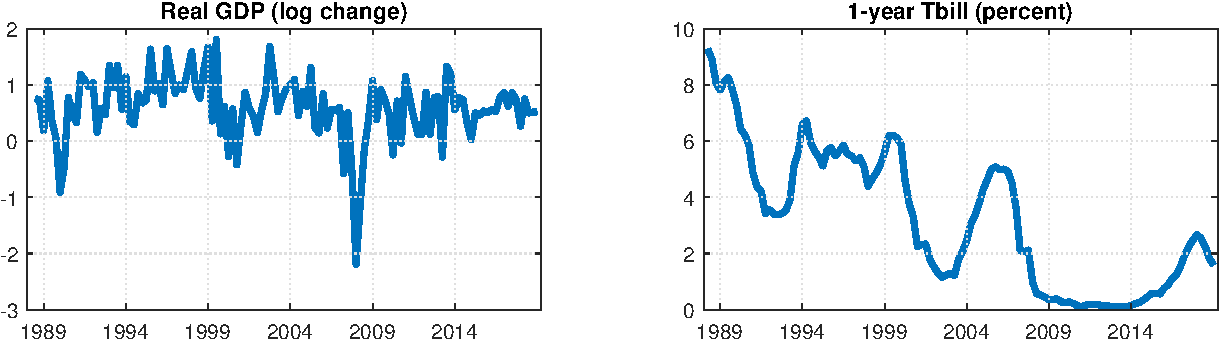
\includegraphics[width=.85\textwidth]{DATA_BivariateVAR.pdf}
\end{figure}
\end{frame}

%------------------------------------------

\begin{frame}
{\textbf{A simple bivariate VAR\ model}}\medskip 

\begin{itemize}
\item As both GDP growth an the 1-year rate are non-zero means, we fit the
data with a VAR(1) with a constant\medskip 
\begin{equation*}
\begin{bmatrix}
y_{t} \\ 
\pi _{t}%
\end{bmatrix}%
=%
\begin{bmatrix}
\alpha _{y} \\ 
\alpha _{\pi }%
\end{bmatrix}%
+\left[ 
\begin{array}{cc}
\phi _{11} & \phi _{12} \\ 
\phi _{21} & \phi _{22}%
\end{array}%
\right] 
\begin{bmatrix}
y_{t-1} \\ 
\pi _{t-1}%
\end{bmatrix}%
+%
\begin{bmatrix}
u_{t}^{y} \\ 
u_{t}^{\pi }%
\end{bmatrix}%
\end{equation*}%
\bigskip

\item This means we will estimate the following parameters\smallskip

\begin{itemize}
\item $2+4$ coefficients, namely the elements of $\alpha $ and $\Phi $%
\medskip

\item $2$ variances of the reduced-form residuals, namely $\sigma _{y}^{2}$
and $\sigma _{\pi }^{2}$\medskip

\item $1$ covariance of the reduced-form residuals, namely $\sigma _{y\pi }$%
\bigskip \smallskip
\end{itemize}

\item We will store these coefficients in two Matlab matrices\medskip 
\begin{equation*}
\text{\colorbox{script!80}{\small\texttt{F}}}=\left[ 
\begin{array}{ccc}
\alpha _{1} & \phi _{11} & \phi _{12} \\ 
\alpha _{2} & \phi _{21} & \phi _{22}%
\end{array}%
\right] \ \ \ \ \ \ \ \text{\colorbox{script!80}{\small\texttt{sigma}}}=%
\left[ 
\begin{array}{cc}
\sigma _{y}^{2} & \sigma _{yr}^{2} \\ 
\sigma _{yr}^{2} & \sigma _{r}^{2}%
\end{array}%
\right]
\end{equation*}
\end{itemize}
\end{frame}

%------------------------------------------

\begin{frame}
{\textbf{A simple bivariate VAR\ model}}\medskip

\begin{itemize}
\item In Matlab we store the data in the matrix \colorbox{script!80}{\small%
\texttt{X}}%
\begin{equation*}
\text{\colorbox{script!80}{\small\texttt{X}}}=\left[ 
\begin{array}{cc}
y_{1} & r_{1} \\ 
y_{2} & r_{2} \\ 
... & ... \\ 
y_{T} & r_{T}%
\end{array}%
\right] =\left( y_{t}^{\prime },r_{t}^{\prime }\right) =x_{t}^{\prime }
\end{equation*}

\item The VAR\ can then be easily estimated with a few lines of code\medskip

\begin{minipage}[b]{.9\textwidth}
\todo[color=script!80,inline,caption={short for LoTds}]{\small\ttfamily
\hspace{1mm}\textcolor{matlabgreen}{\% Set the deterministic variable in the VAR (1=constant, 2=trend) }\\
\hspace{1mm}det = 1; \\
\hspace{1mm}\textcolor{matlabgreen}{\% Set number of nlags }\\
\hspace{1mm}nlags = 12; \\
\hspace{1mm}\textcolor{matlabgreen}{\% Estimate VAR by OLS }\\
\hspace{1mm}[VAR, VARopt] = VARmodel(ENDO,nlags,det); \\
}\end{minipage}
\end{itemize}
\end{frame}

%------------------------------------------

\begin{xframe}
\frametitle{A simple bivariate VAR\ model: VAR\ output}\medskip

\begin{itemize}
\item The code estimates the VAR equation by equation with OLS \bigskip\ 

\item Results are stored in the \colorbox{script!80}{\small\texttt{VAR}} and %
\colorbox{script!80}{\small\texttt{VARopt}} structures\bigskip

\item The six estimated parameters (i.e. $\alpha $ and $\Phi $)\ can be
printed at screen by simply typing \colorbox{script!80}{\small%
\texttt{disp(VAR.Ft)}} to get \medskip

\begin{minipage}{\textwidth}
\begin{verbatim}
>> disp(VAR.F)
    0.3630    0.3788    0.0041
   -0.0729    0.2607    0.9541
\end{verbatim}
\end{minipage}

\bigskip

\item For the three elements of $\Sigma _{u}$ type \colorbox{script!80}{%
\small \texttt{disp(VAR.sigma)}} to get \medskip

\begin{minipage}{\textwidth}
\begin{verbatim}
>> disp(VAR.sigma)
    0.2891    0.0782
    0.0782    0.1473
\end{verbatim}
\end{minipage}
\end{itemize}
\end{xframe}

%------------------------------------------

\begin{frame}
{\textbf{OLS\ estimation: Typical VAR\ output (cont'd)}}\medskip

\begin{itemize}
\item The off-diagonal elements of $\Sigma $ capture the {%
\tikz[tstyle]{\node[nstyle](node1){\textbf{average}};}} contemporaneous
relation between the endogenous variables 
\begin{tikzpicture}[tpstyle]
\draw[pencil,decoration={segment length=1.5pt}] ([yshift=-2pt]node1.south west) to ([yshift=-2pt]node1.south east);
\end{tikzpicture}\medskip

\begin{table}[tbph]
\centering%
\begin{tabular}{rrr}
\toprule & GDP growth ($u_{y}$) & 1-year T-Bill($u_{r}$) \\ 
\midrule Real GDP ($u_{y}$) & 0.2891 & {\tikz[tstyle]{%
\node[nstyle](node1){0.0782};}} \\ 
1-year T-Bill($u_{r}$) & 0.0782 & 0.1473 \\ 
\bottomrule &  & 
\end{tabular}%
\end{table}
\pause

\begin{tikzpicture}[tpstyle]
\node[pencil,draw, minimum height=0.5cm, minimum width=1.1cm] (box1) at (node1) {};
\draw[arrow,opacity=1] (box1.east) to[bend left] +(0.9,-0.1) node[gold,anchor=west,opacity=1] {\footnotesize{\textbf{\augiefamily Cov(u\tiny{y},\footnotesize,u\tiny{r}\footnotesize)>0}}};
\end{tikzpicture}

\item In our example output growth and inflation are contemporaneously
positively correlated\smallskip

\begin{itemize}
\item It means that, on average, when GDP growth increases inflation
increases, too\bigskip \pause
\end{itemize}

\item Does it mean that a shock to output always increase
inflation?\smallskip

\begin{itemize}
\item No! Recall that reduced from residuals are not informative about
structural shocks
\end{itemize}
\end{itemize}
\end{frame}

%------------------------------------------

\begin{frame}
{\textbf{Model checking \& tuning}}\bigskip \medskip

\begin{itemize}
\item These notes do not cover this aspect in detail but... \bigskip

\item ... before interpreting the VAR results you should check a number of
assumptions\bigskip \pause

\item Loosely speaking, you need to check that the reduced-form residuals
are\smallskip

\begin{itemize}
\item Normally distributed\medskip

\item Not autocorrelated\medskip

\item Not heteroskedastic (i.e., have constant variance)\bigskip \pause
\end{itemize}

\item ... and that the VAR is stable
\end{itemize}
\end{frame}

%------------------------------------------

\begin{xframe}
\frametitle{Stability and equilibrium}

\begin{itemize}
\item We've already seen that a VAR\ is stable when $\left\vert eig(\Phi
)\right\vert <1$\smallskip

\begin{itemize}
\item If this condition is not met, the infinite sums in the Wold
representation do not converge\bigskip
\end{itemize}

\pause

\item You can check the maximum value of $\Phi $'s eigenvalues in the %
\colorbox{script!80}{\small\texttt{VAR}} structure, by typing %
\colorbox{script!80}{\small\texttt{disp(VAR.maxEig)}} to get \medskip

\begin{minipage}{0.7\textwidth}
\small\begin{verbatim}
>> disp(VAR.maxEig)
    0.9559
\end{verbatim}
\end{minipage}\pause\medskip

\item You can also check all of $\Phi $'s eigenvalues by executing Matlab's %
\colorbox{script!80}{\small\texttt{eig}} function on the VAR's companion
matrix \colorbox{script!80}{\small\texttt{Fcomp}} (which, note, is built
excluding the constant from \colorbox{script!80}{\small\texttt{F}}).\bigskip

\item In practice:\medskip

\begin{minipage}{0.7\textwidth}
\small\begin{verbatim}
>> disp(eig(VAR.Fcomp))
    0.3769
    0.9559
\end{verbatim}
\end{minipage}
\end{itemize}
\end{xframe}

%------------------------------------------

\begin{frame}
{\textbf{Stability and equilibrium (cont'd)}}

\begin{itemize}
\item As our VAR\ is stable, its Wold representation will converge to the
(finite)\ unconditional mean of the data\bigskip

\item To see that, first consider the Wold representation in the presence of
a constant%
\begin{equation*}
x_{t}={\Phi ^{t}x_{0}+\sum\limits_{j=0}^{t-1}\Phi ^{t}\alpha }+{%
\sum\limits_{j=0}^{t-1}\Phi ^{j}B{\varepsilon _{t-j}}}
\end{equation*}
\vspace{-.1cm}

\item For $t$ large enough and taking expectations we get 
\begin{equation*}
\mathbb{E}\left[ x_{t}\right] ={\sum\limits_{j=0}^{t-1}\Phi ^{t}\alpha =}%
\left( I_{2}-\Phi \right) ^{-1}\alpha
\end{equation*}
\vspace{-.1cm}

\item In absence of shocks, the VAR's variable will converge to its
equilibrium $\left( I_{2}-\Phi \right) ^{-1}\alpha $ at a rate that depends
on $\Phi $
\end{itemize}
\end{frame}

%------------------------------------------

\begin{frame}
{\textbf{Examples of different identification schemes}}

\begin{itemize}
\item Zero short-run restrictions

\begin{itemize}
\item Stock \& Watson\ (2001). \textquotedblleft Vector
Autoregressions,\textquotedblright\ \emph{Journal of Economic Perspectives}%
\medskip
\end{itemize}

\item Zero long-run restrictions

\begin{itemize}
\item Blanchard \&\ Quah (1989). \textquotedblleft The Dynamic Effects of
Aggregate Demand and Supply Disturbances\textquotedblright , \emph{American
Economic Review}\medskip
\end{itemize}

\item Sign Restrictions

\begin{itemize}
\item Uhlig (2005). \textquotedblleft What are the effects of monetary
policy on output? Results from an agnostic identification
procedure,\textquotedblright\ \emph{Journal of Monetary Economics}\medskip
\end{itemize}

\item External instruments

\begin{itemize}
\item Gertler and Karadi (2015). \textquotedblleft What are the effects of
monetary policy on output? Results from an agnostic identification
procedure,\textquotedblright\ \emph{American Economic Journal:\
Macroeconomics}\medskip
\end{itemize}

\item External instruments\ \&\ Sign restrictions

\begin{itemize}
\item Cesa-Bianchi and Sokol (2020). \textquotedblleft Financial Shocks,
Credit Spreads, and the International Credit Channel,\textquotedblright\ 
\emph{Unpublished manuscript}
\end{itemize}
\end{itemize}
\end{frame}

%------------------------------------------

\subsection{Stock \& Watson\ (2001, JEP)}

\begin{frame}
\vspace{3cm} \color{title}\centering{\huge \textbf{Practical Examples}}%
\bigskip

\color{note}\centering{\Large \textbf{Stock \& Watson\ (2001, JEP)}}
\end{frame}

%------------------------------------------

\begin{frame}
{\textbf{Stock \& Watson\ (2001): Zero short-run restrictions}}\bigskip

\begin{itemize}
\item Stock \& Watson\ (2001). \textquotedblleft Vector
Autoregressions,\textquotedblright\ \textit{Journal of Economic Perspectives}%
\bigskip

\item US\ quarterly data from 1960QI to 2000Q4
\end{itemize}

\begin{figure}[h]
\centering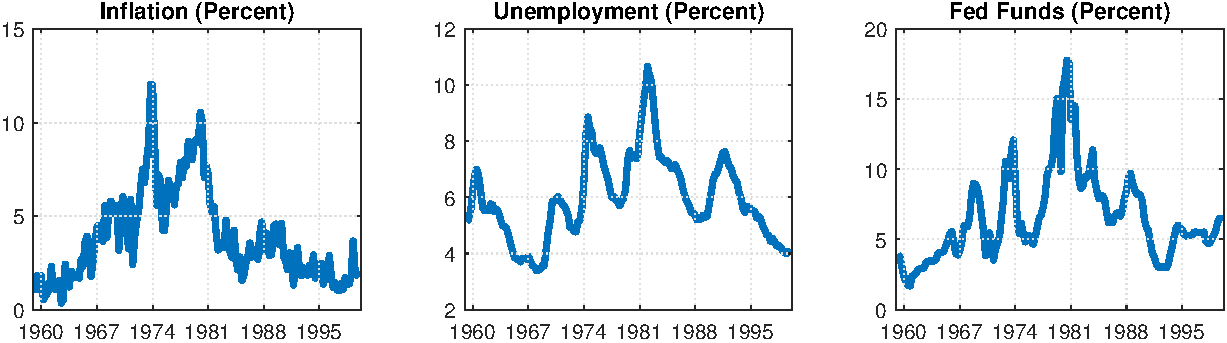
\includegraphics[width=.85\textwidth]{SW_DATA.pdf}
\end{figure}
\end{frame}

%------------------------------------------

\begin{frame}
{\textbf{Monetary policy shocks, inflation and unemployment}}\bigskip\bigskip

\begin{itemize}
\item \textbf{Objective} \ Infer the causal influence of monetary policy on
unemployment and inflation\bigskip\pause

\item Assume a VAR with $p=4$ with inflation ($\pi_t$), unemployment ($u_t$%
), and the fed funds rate ($r_t$)\bigskip

\item \textbf{Key identifying assumptions}\smallskip

\begin{itemize}
\item MP\ ($r_{t}$) reacts contemporaneously to movements in inflation and
in unemployment\medskip

\item MP shocks ($\varepsilon_{3t}$) do not affect inflation and
unemployment within the quarter of the shock\smallskip \pause%
\begin{equation*}
\begin{bmatrix}
\pi _{t} \\ 
u_{t} \\ 
r_{t}%
\end{bmatrix}%
=\sum_{p=1}^4 \Phi_p x_{t-p} +\left[ 
\begin{array}{ccc}
b_{11} & 0 & 0 \\ 
b_{21} & b_{22} & 0 \\ 
b_{31} & b_{32} & b_{33}%
\end{array}%
\right] 
\begin{bmatrix}
\varepsilon^{1}_{t} \\ 
\varepsilon^{2}_{t} \\ 
\varepsilon^{MonPol}_{t}%
\end{bmatrix}%
\end{equation*}
\end{itemize}
\end{itemize}
\end{frame}

%------------------------------------------

\begin{frame}
{\textbf{Monetary policy shocks, inflation and unemployment}}\vspace{-.1cm}

\begin{itemize}
\item In Matlab, set lag length to $4$ and estimate a VAR with a constant
\medskip

\begin{minipage}[b]{.9\textwidth}
\todo[color=script!80,inline,caption={short for LoTds}]{\small\ttfamily
\hspace{1mm}\textcolor{matlabgreen}{\% Set up and estimate VAR }\\
\hspace{1mm}det = 1; \\
\hspace{1mm}nlags = 4; \\
\hspace{1mm}[VAR, VARopt] = VARmodel(X,nlags,det); \\
}\end{minipage}

\medskip

\item Then set the option for recursive identification \colorbox{script!80}{%
\small\texttt{VARopt.ident ='short'}} and compute the $IR$ with the %
\colorbox{script!80}{\small\texttt{VARir}} function. Note that the ordering
of the variables matter!\medskip

\begin{minipage}[b]{.9\textwidth}
\todo[color=script!80,inline,caption={short for LoTds}]{\small\ttfamily
\hspace{1mm}\textcolor{matlabgreen}{\% For zero contemporaneous restrictions set: }\\
\hspace{1mm}VARopt.ident = \textcolor{matlabpurple}{'short'}; \\
\hspace{1mm}\textcolor{matlabgreen}{\% Compute IR }\\
\hspace{1mm}[IR, VAR] = VARir(VAR,VARopt); \\
}\end{minipage}

\medskip

\item The \colorbox{script!80}{\small\texttt{VARirband}} function allows tlo
compute confidence intervals\medskip

\begin{minipage}[b]{.9\textwidth}
\todo[color=script!80,inline,caption={short for LoTds}]{\small\ttfamily
\hspace{1mm}\textcolor{matlabgreen}{\% Compute IR }\\
\hspace{1mm}[IR, VAR] = VARir(VAR,VARopt); \\
}\end{minipage}
\end{itemize}
\end{frame}

%------------------------------------------

\begin{frame}
{\textbf{The effect of a monetary policy shock}}

\begin{itemize}
\item Monetary policy shock raises inflation in the short run (price puzzle)
and increases unemployment
\end{itemize}

\begin{figure}[h]
\centering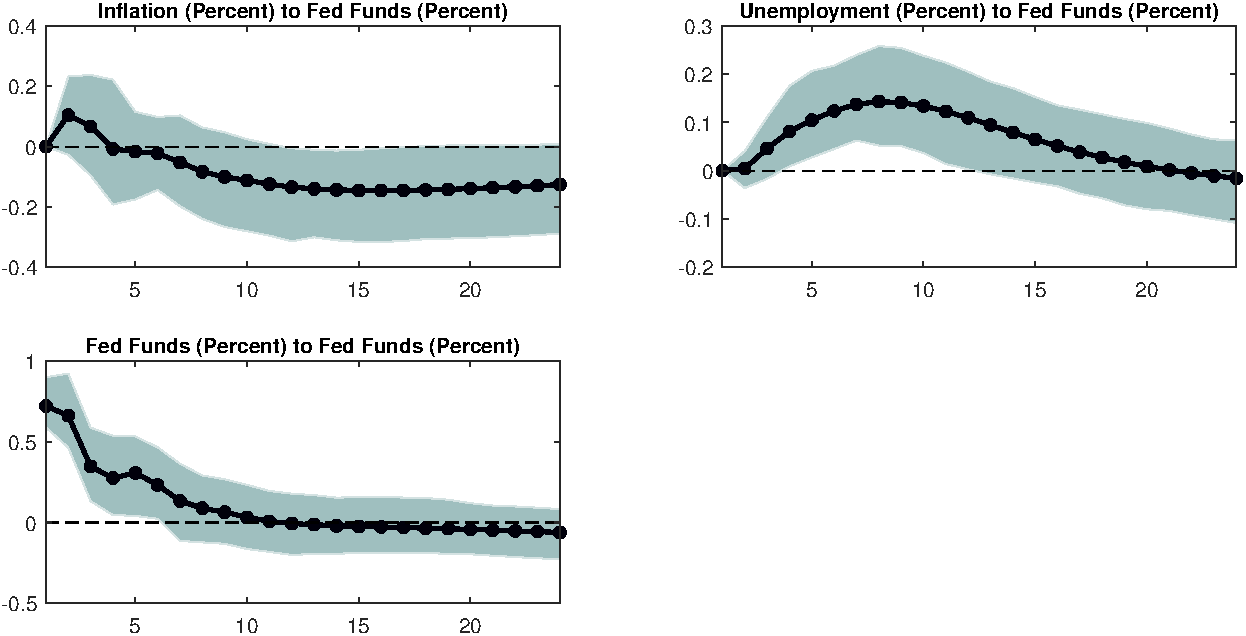
\includegraphics[width=.75\textwidth]{SW_IR_3.pdf}
\end{figure}
\end{frame}

%------------------------------------------

\begin{frame}
{\textbf{The other two shocks are identified by definition... but how can we
interpret them?}}\bigskip\bigskip

\begin{itemize}
\item How about $\varepsilon^{1}_{t}$ and $\varepsilon^2_{t}$? \smallskip

\begin{itemize}
\item The shock $\varepsilon^{1}_{t}$ affects all variables
contemporaneously\medskip

\item The shock $\varepsilon^2_{t}$ affects $r_{t}$ contemporaneously but
not $\pi _{t}$\pause\bigskip
\end{itemize}

\item Can we interpret these shocks? Are the assumptions consistent with any
theoretical mechanism? \pause\bigskip

\item Some shocks may be better identified than others
\end{itemize}
\end{frame}

%------------------------------------------

\begin{frame}
{\textbf{The other two shocks are identified by definition... but how can we
interpret them?}}

\begin{itemize}
\item Shock to $\varepsilon^1_{t}$ behaves as a negative aggregate supply
shock
\end{itemize}

\begin{figure}[h]
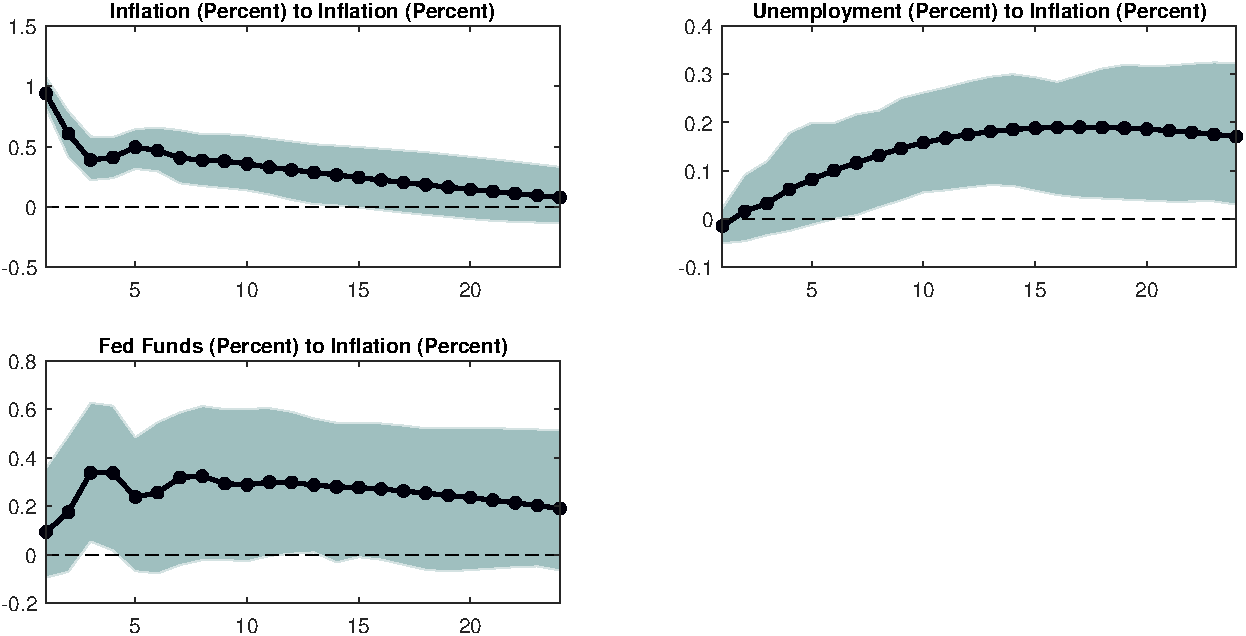
\includegraphics[width=.75\textwidth]{SW_IR_1.pdf}
\end{figure}
\end{frame}

%------------------------------------------

\begin{frame}
{\textbf{The other two shocks are identified by definition... but how can we
interpret them?}}

\begin{itemize}
\item Shock to $\varepsilon^2_{t}$ behaves as a negative aggregate demand
shock
\end{itemize}

\begin{figure}[h]
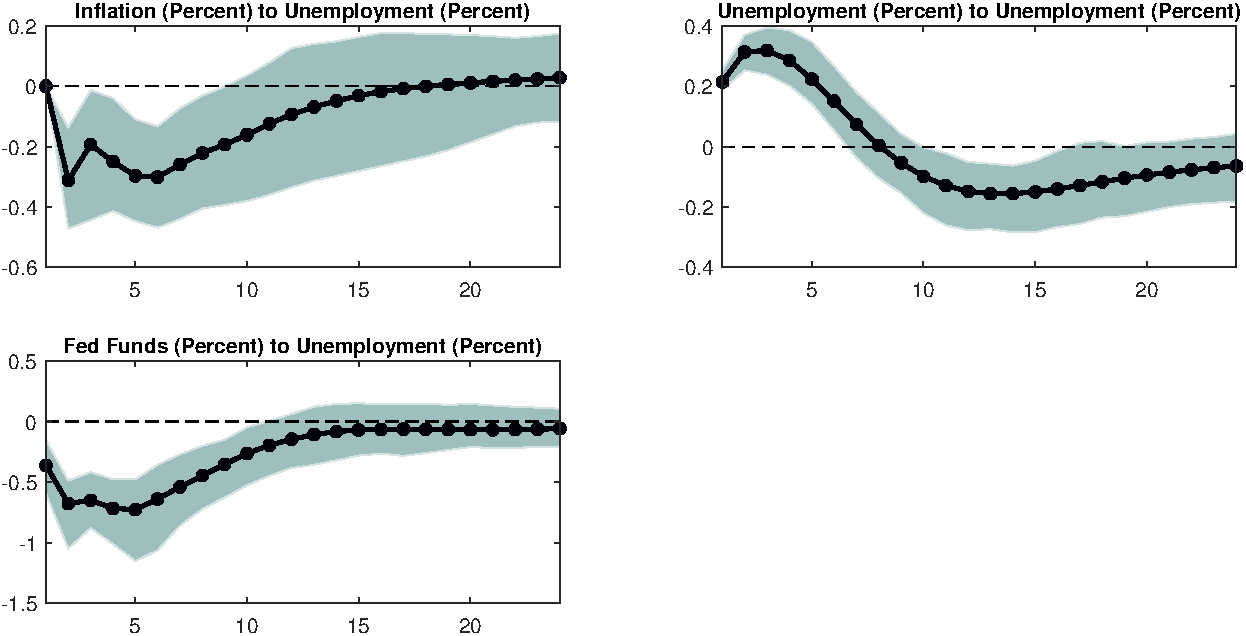
\includegraphics[width=.75\textwidth]{SW_IR_2.pdf}
\end{figure}
\end{frame}

%------------------------------------------

\begin{frame}
{\textbf{Forecast error variance \& Historical decompositions}}\bigskip

\begin{itemize}
\item In Matlab, set compute the $VD$ with the \colorbox{script!80}{\small%
\texttt{VARvd}} function\medskip

\begin{minipage}[b]{.9\textwidth}
\todo[color=script!80,inline,caption={short for LoTds}]{\small\ttfamily
\hspace{1mm}\textcolor{matlabgreen}{\% Compute VD }\\
\hspace{1mm}[VD, VAR] = VARvd(VAR,VARopt); \\
}\end{minipage}

\bigskip

\item Similarly, the $HD$ can be computed with the \colorbox{script!80}{%
\small\texttt{VARhd}} function\medskip

\begin{minipage}[b]{.9\textwidth}
\todo[color=script!80,inline,caption={short for LoTds}]{\small\ttfamily
\hspace{1mm}\textcolor{matlabgreen}{\% Compute HD}\\
\hspace{1mm}[HD, VAR] = VARhd(VAR,VARopt); \\
}\end{minipage}
\end{itemize}
\end{frame}

%------------------------------------------

\begin{frame}
{\textbf{Forecast error variance decomposition}}\medskip

\begin{figure}[h]
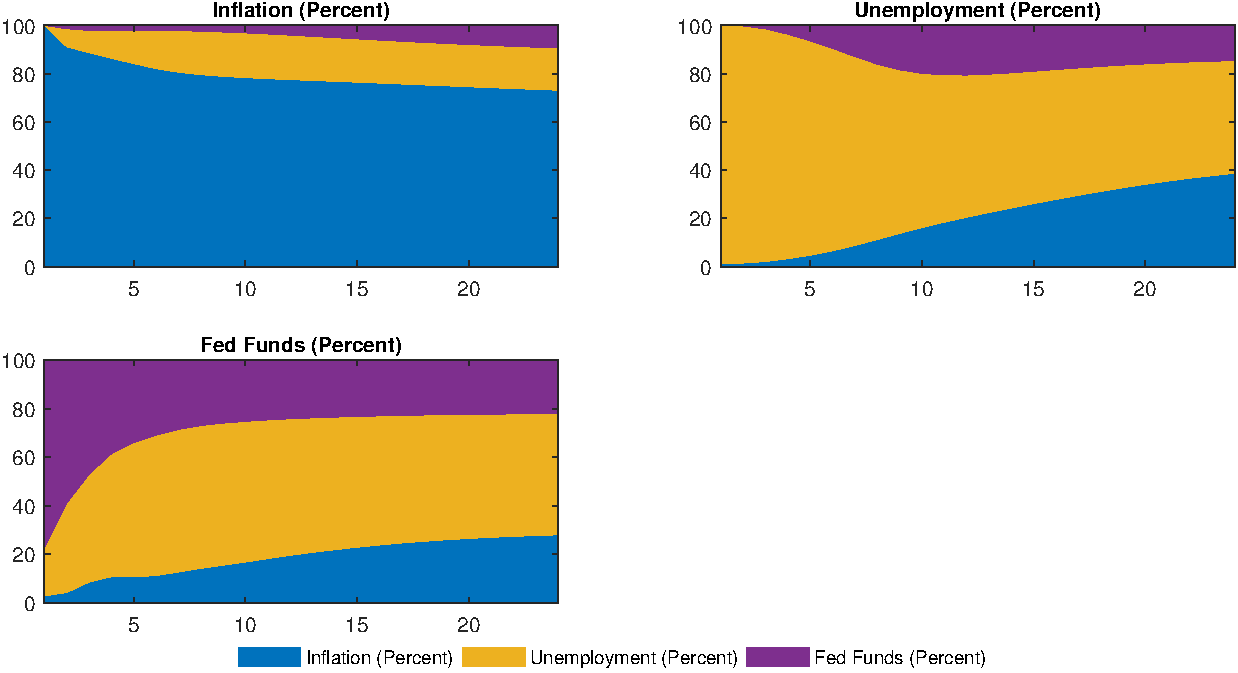
\includegraphics[width=.75\textwidth]{SW_VD.pdf}
\end{figure}
\end{frame}

%------------------------------------------

\begin{frame}
{\textbf{Historical decomposition}}\medskip

\begin{figure}[h]
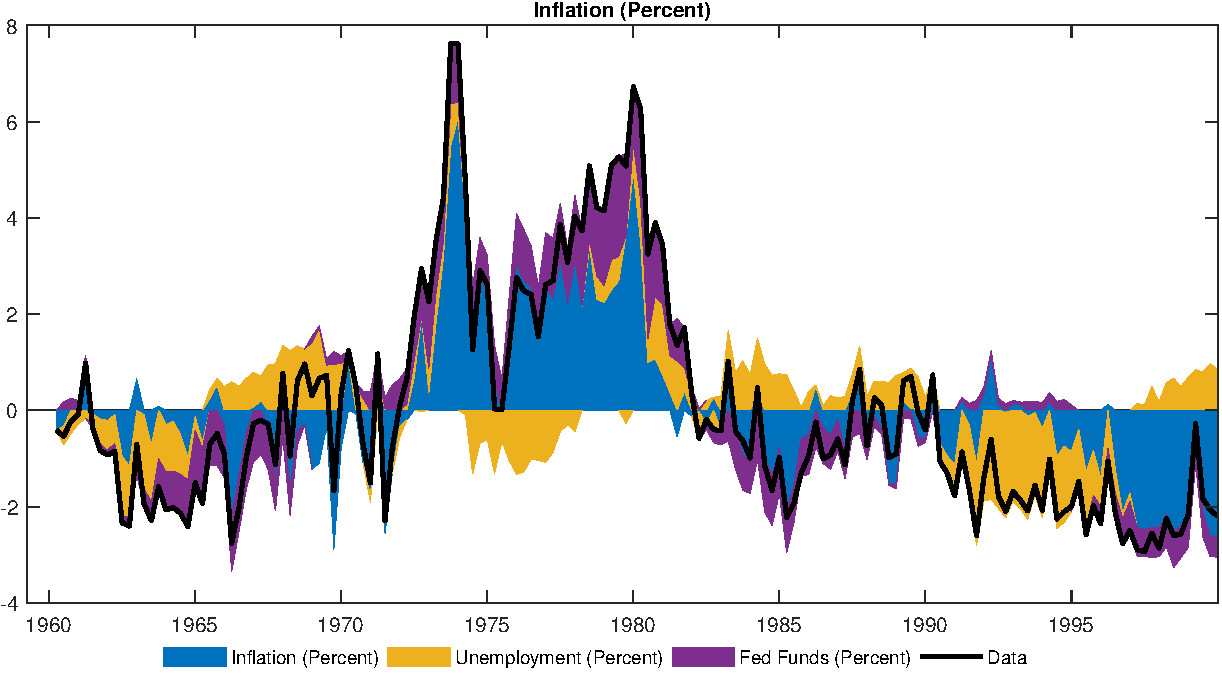
\includegraphics[width=.75\textwidth]{SW_HD_1.pdf}
\end{figure}
\end{frame}

%------------------------------------------

\begin{frame}
{\textbf{Historical decomposition}}\medskip

\begin{figure}[h]
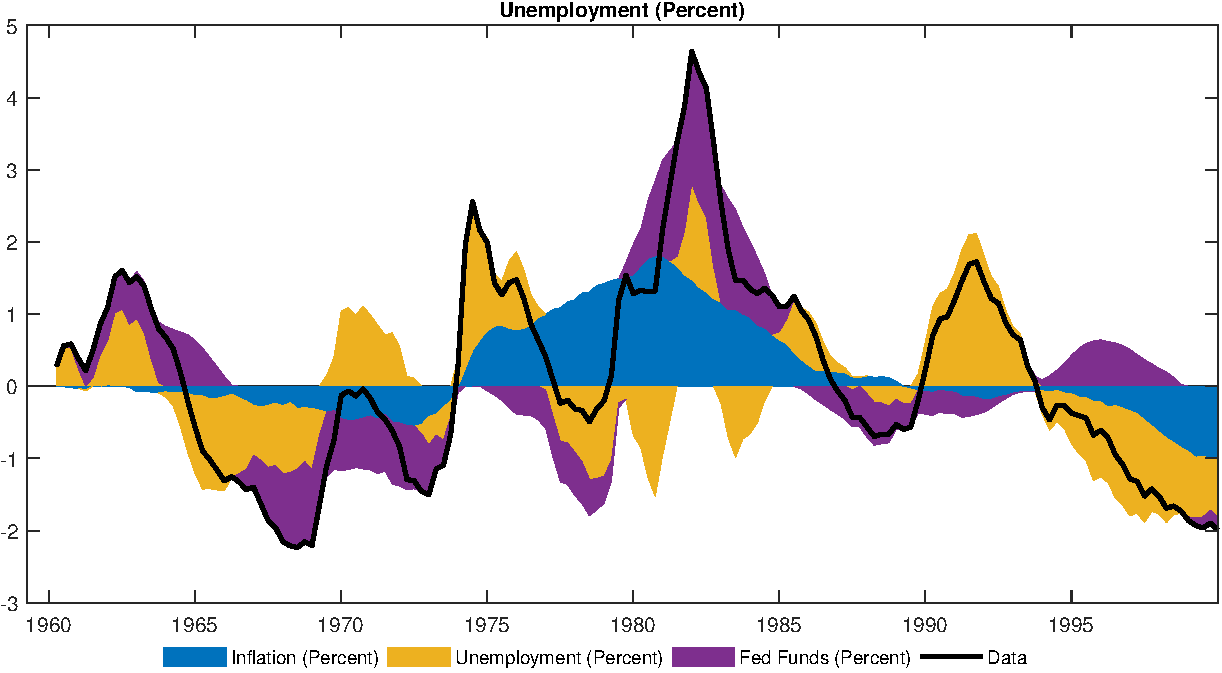
\includegraphics[width=.75\textwidth]{SW_HD_2.pdf}
\end{figure}
\end{frame}

%------------------------------------------

\begin{frame}
{\textbf{Historical decomposition}}\medskip

\begin{figure}[h]
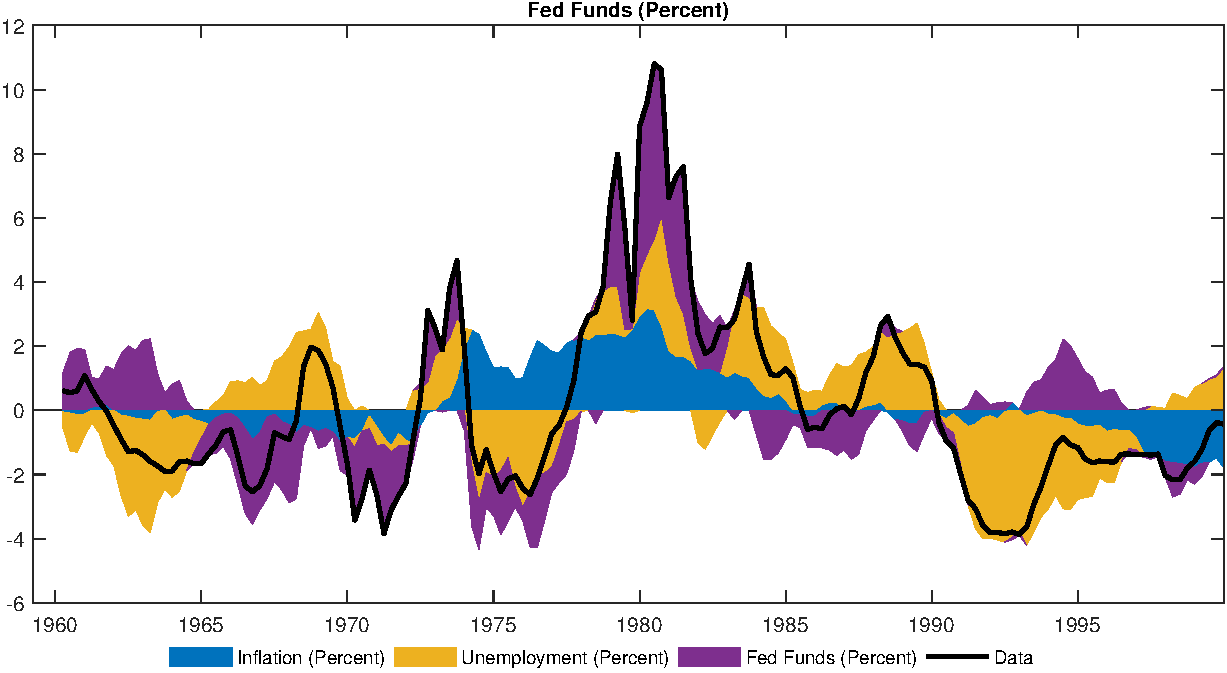
\includegraphics[width=.75\textwidth]{SW_HD_3.pdf}
\end{figure}
\end{frame}

%------------------------------------------

\subsection{Blanchard \&\ Quah (1989, AER)}

\begin{frame}
\vspace{3cm} \color{title}\centering{\huge \textbf{Practical Examples}}%
\bigskip

\color{note}\centering{\Large \textbf{Blanchard \&\ Quah (1989, AER)}}
\end{frame}

%------------------------------------------

\begin{frame}
{\textbf{Blanchard \&\ Quah (1989): Zero long-run restrictions}}

\begin{itemize}
\item Blanchard \&\ Quah (1989). \textquotedblleft The Dynamic Effects of
Aggregate Demand and Supply Disturbances\textquotedblright , \emph{American
Economic Review}\bigskip

\item US\ quarterly data from 1948Q1 to 1987Q4\bigskip

\begin{figure}[h]
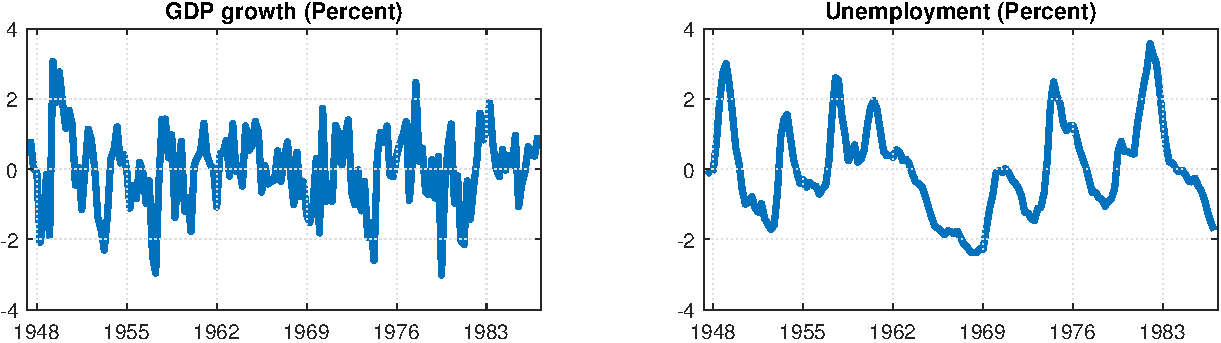
\includegraphics[width=.85\textwidth]{BQ_DATA.pdf}
\end{figure}
\end{itemize}
\end{frame}

%------------------------------------------

\begin{frame}
{\textbf{What is the effect of demand and supply shocks?}}\bigskip

\begin{itemize}
\item \textbf{Objective} Identify the effects of demand and supply shocks on
output and unemployment\bigskip \pause

\item Assume a bivariate VAR with $p=8$ with output growth ($y_{t}$) and
unemployment ($u_{t}$)\bigskip

\item \textbf{Key identifying assumption} \ Demand-side shocks have no
long-run effect on the level of output, while supply-side shocks do\smallskip

\begin{itemize}
\item Blanchard \&\ Quah impose zero long-run restrictions on the cumulative
effect of demand shocks on output growth (i.e. on output level) to identify
the shocks\medskip 
\begin{equation*}
\begin{bmatrix}
y_{t,t+\infty } \\ 
u_{t,t+\infty }%
\end{bmatrix}%
=\left[ 
\begin{array}{cc}
c_{11} & 0 \\ 
c_{21} & c_{22}%
\end{array}%
\right] 
\begin{bmatrix}
\varepsilon _{t}^{Supply} \\ 
\varepsilon _{t}^{Demand}%
\end{bmatrix}%
\end{equation*}
\end{itemize}
\end{itemize}
\end{frame}

%------------------------------------------

\begin{frame}
{\textbf{Monetary policy shocks, inflation and unemployment}}\vspace{-.1cm}

\begin{itemize}
\item In Matlab, set lag length to $8$ and estimate a VAR with a constant
\medskip

\begin{minipage}[b]{.9\textwidth}
\todo[color=script!80,inline,caption={short for LoTds}]{\small\ttfamily
\hspace{1mm}\textcolor{matlabgreen}{\% Set up and estimate VAR }\\
\hspace{1mm}det = 1; \\
\hspace{1mm}nlags = 8; \\
\hspace{1mm}[VAR, VARopt] = VARmodel(X,nlags,det); \\
}\end{minipage}

\medskip

\item Then set the option for zero long-run restrictions %
\colorbox{script!80}{\small\texttt{VARopt.ident ='long'}} and compute the $%
IR $ with the \colorbox{script!80}{\small\texttt{VARir}} function. Note that
the ordering of the variables matter!\medskip

\begin{minipage}[b]{.9\textwidth}
\todo[color=script!80,inline,caption={short for LoTds}]{\small\ttfamily
\hspace{1mm}\textcolor{matlabgreen}{\% For zero contemporaneous restrictions set: }\\
\hspace{1mm}VARopt.ident = \textcolor{matlabpurple}{'long'}; \\
\hspace{1mm}\textcolor{matlabgreen}{\% Compute IR }\\
\hspace{1mm}[IR, VAR] = VARir(VAR,VARopt); \\
}\end{minipage}

\medskip

\item The $B$ matrix implied by the zero long-run restrictions is stored in %
\colorbox{script!80}{\small\texttt{VAR.B}}
\end{itemize}
\end{frame}

%------------------------------------------

\begin{frame}
{\textbf{Aggregate supply shock}}

\begin{itemize}
\item Aggregate supply shock initially increases unemployment (puzzle of
hours to productivity shocks)
\end{itemize}

\begin{figure}[h]
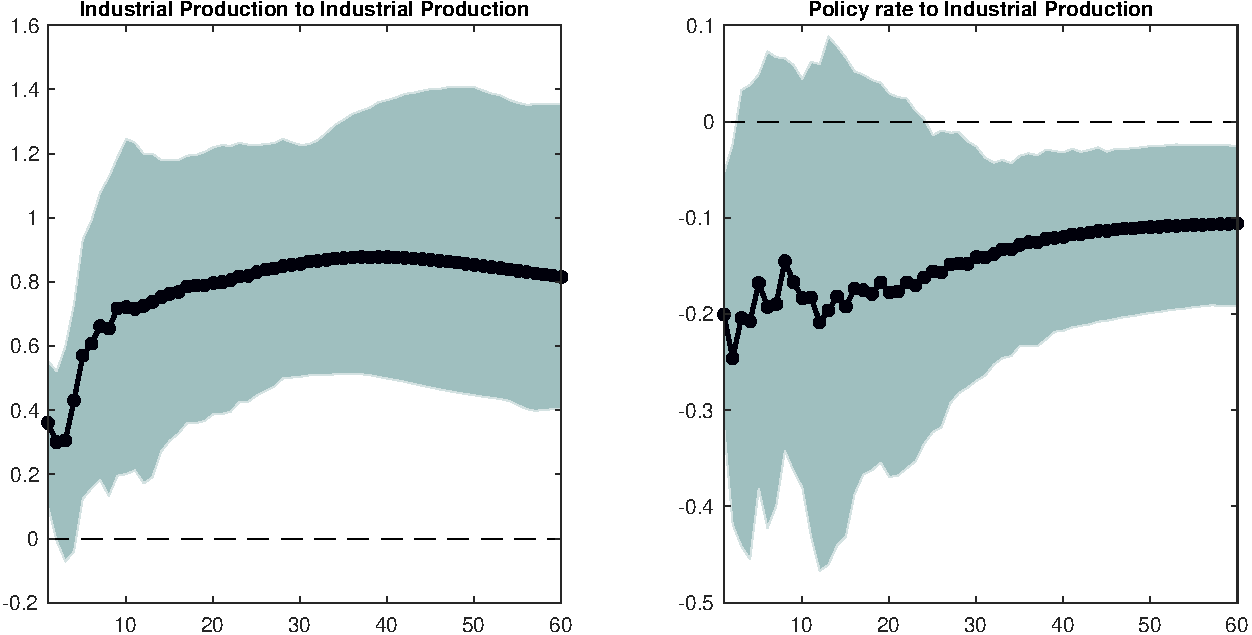
\includegraphics[width=.8\textwidth]{BQ_IR_1.pdf}
\end{figure}
\end{frame}

%------------------------------------------

\begin{frame}
{\textbf{Aggregate demand shock}}

\begin{itemize}
\item Aggregate demand shocks have a hump-shaped effect on output and
unemployment
\end{itemize}

\begin{figure}[h]
\vspace{.3cm}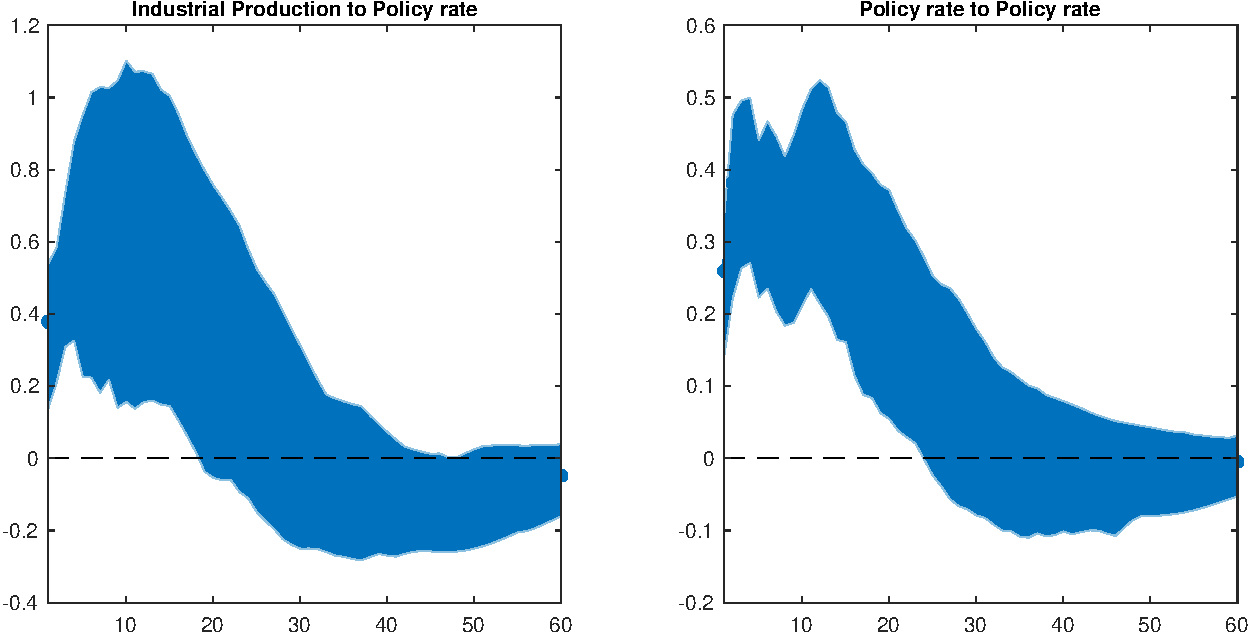
\includegraphics[width=.8\textwidth]{BQ_IR_2.pdf}
\end{figure}
\end{frame}

%------------------------------------------

\begin{frame}
{\textbf{What is the long run effect of demand and supply shocks on output
level?}}

\begin{itemize}
\item Blanchard \&\ Quah report (Figure 1)\ the cumulative sum of the
impulse responses of output growth (i.e. the response of output
level)\medskip

\item By assumption, it should be zero for demand shocks \ \ding{52} \vspace{%
-0.1cm}\pause
\end{itemize}

\begin{figure}[h]
\vspace{.3cm}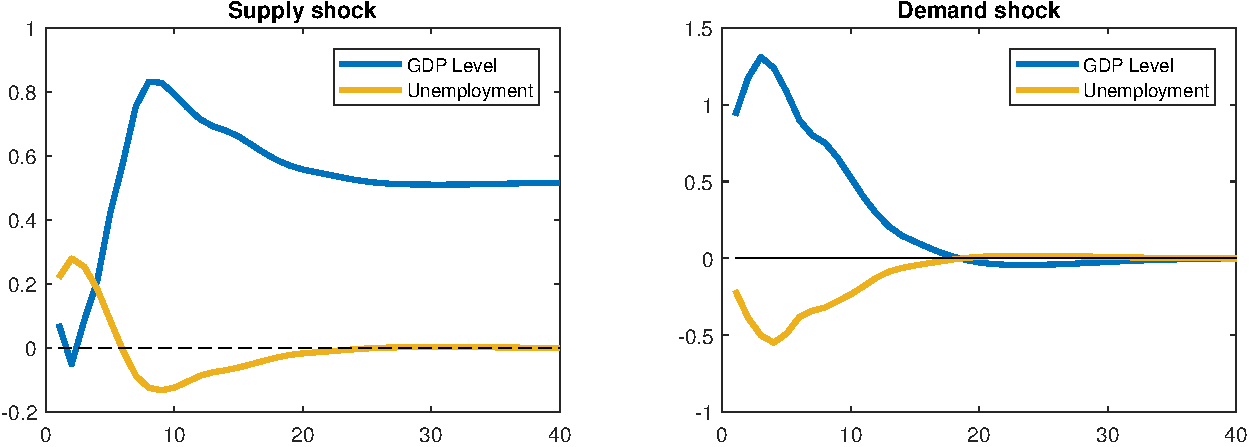
\includegraphics[width=.8\textwidth]{BQ_Replication.pdf}
\end{figure}
\end{frame}

%------------------------------------------

\subsection{Uhlig (2005, JME)}

\begin{frame}
\vspace{3cm} \color{title}\centering{\huge \textbf{Practical Examples}}%
\bigskip

\color{note}\centering{\Large \textbf{Uhlig (2005, JME)}}
\end{frame}

%------------------------------------------

\begin{frame}
{\textbf{Uhlig (2005, JME): Sign restrictions}}

\begin{minipage}{0.4\textwidth}
\bigskip
\begin{itemize}
\item Uhlig (2005). \textquotedblleft What are the effects of monetary policy on output? Results from an agnostic identification
procedure,\textquotedblright\ \emph{Journal of Monetary Economics} \bigskip

\item US\ monthly data from 1965M1 to 2003M12
\end{itemize}
\end{minipage}
\quad 
\begin{minipage}{0.55\textwidth}
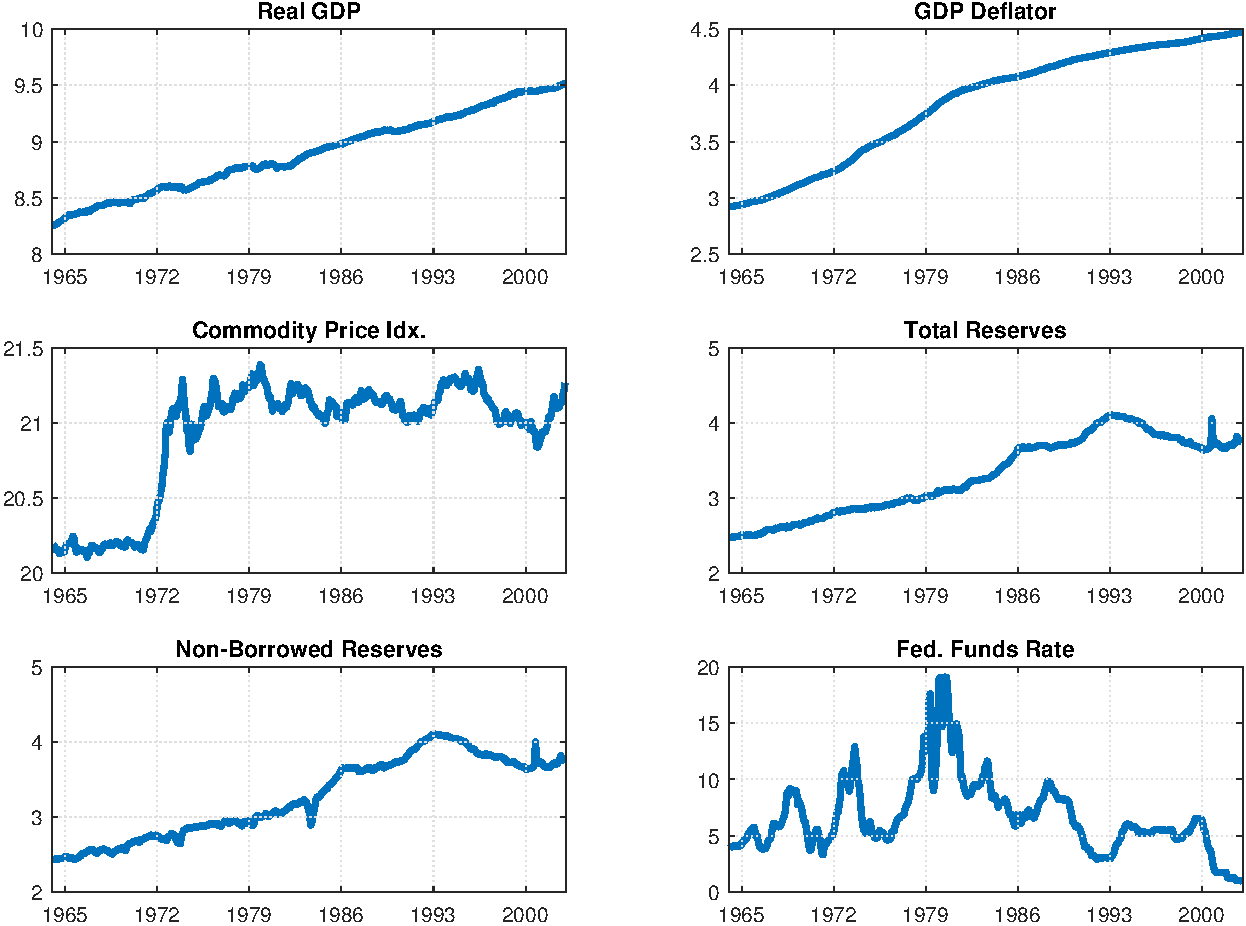
\includegraphics[width=\textwidth]{Uhlig_DATA.pdf}
\end{minipage}
\end{frame}

%------------------------------------------

\begin{frame}
{\textbf{What are the effects of monetary policy on output?}}\medskip

\begin{itemize}
\item \textbf{Objective} \ Infer the causal influence of monetary policy on
real GDP\bigskip \pause

\item Assume a VAR with $p=12$ with real GDP, real GDP deflator, a commodity
price index, total reserves, non-borrowed reserves, and the fed. funds
rate\bigskip

\item \textbf{Key identifying assumptions} According to conventional wisdom,
monetary contractions should\smallskip

\begin{itemize}
\item Raise the federal funds rate\smallskip

\item Lower prices\smallskip

\item Decrease non-borrowed reserves\bigskip
\end{itemize}

\item Real GDP\ is left unrestricted
\end{itemize}
\end{frame}

%------------------------------------------

\begin{frame}
{\textbf{Monetary policy shock:\ The sign restrictions}}\bigskip

\begin{itemize}
\item Uhlig imposes the following sign restrictions on the impulse responses
of the VAR%
\begin{equation*}
\begin{tabular}{lc}
\hline
\addlinespace & Monetary Policy Shock \\ \hline
\addlinespace Real GDP ($y_{t}$) & ? \\ 
Real GDP\ deflator ($p_{t}$) & $<0$ \\ 
commodity price index, & ? \\ 
total reserves, & ? \\ 
non-borrowed reserves, & $<0$ \\ 
Fed. Funds Rate & $>0$ \\ \hline
\end{tabular}%
\end{equation*}%
\bigskip

\item Restrictions are imposed for $6$ periods
\end{itemize}
\end{frame}

%------------------------------------------

\begin{frame}
{\textbf{Monetary policy shock:\ The sign restrictions}}

\begin{itemize}
\item In Matlab, the sign restrictions can be set as follows\medskip

\begin{minipage}[b]{.9\textwidth}
\todo[color=script!80,inline,caption={short for LoTds}]{\small\ttfamily
\hspace{1mm}\textcolor{matlabgreen}{\% Define the shock names }\\
\hspace{1mm}VARopt.snames = \{\textcolor{matlabpurple}{'Mon. Policy Shock'}\}; \\
\hspace{1mm}\textcolor{matlabgreen}{\% Define sign restrictions : positive 1, negative -1, unrestricted 0 }\\
\hspace{1mm}SIGN = [ 0,0,0,0,0,0;  \textcolor{matlabgreen}{\% Real GDP }\\
\hspace{1mm}-1,0,0,0,0,0;  \textcolor{matlabgreen}{\% Deflator }\\
\hspace{1mm}-1,0,0,0,0,0;  \textcolor{matlabgreen}{\% Commodity Price }\\
\hspace{1mm}0,0,0,0,0,0;  \textcolor{matlabgreen}{\% Total Reserves }\\
\hspace{1mm}-1,0,0,0,0,0;  \textcolor{matlabgreen}{\% NonBorr. Reserves }\\
\hspace{1mm}1,0,0,0,0,0]; \textcolor{matlabgreen}{\% Fed Fund }\\
\hspace{1mm}\textcolor{matlabgreen}{\% Define the number of steps the restrictions are imposed for: }\\
\hspace{1mm}VARopt.sr\_hor = 6; \\
}\end{minipage}

\bigskip

\item The routine is then implemented with the \colorbox{script!80}{\small%
\texttt{SR}} function\medskip

\begin{minipage}[b]{.9\textwidth}
\todo[color=script!80,inline,caption={short for LoTds}]{\small\ttfamily
\hspace{1mm}\textcolor{matlabgreen}{\% The functin SR performs the sign restrictions identification and computes }\\
\hspace{1mm}\textcolor{matlabgreen}{\% IRs, VDs, and HDs. All the results are stored in SRout }\\
\hspace{1mm}SRout = SR(VAR,SIGN,VARopt); \\
}\end{minipage}
\end{itemize}
\end{frame}

%------------------------------------------

\begin{frame}
{\textbf{What happens when you do sign restrictions }}

\begin{itemize}
\item Start drawing orthonormal matrices $Q$ until you find one that
satisfies the restrictions...
\end{itemize}

\begin{figure}[h]
\vspace{.3cm}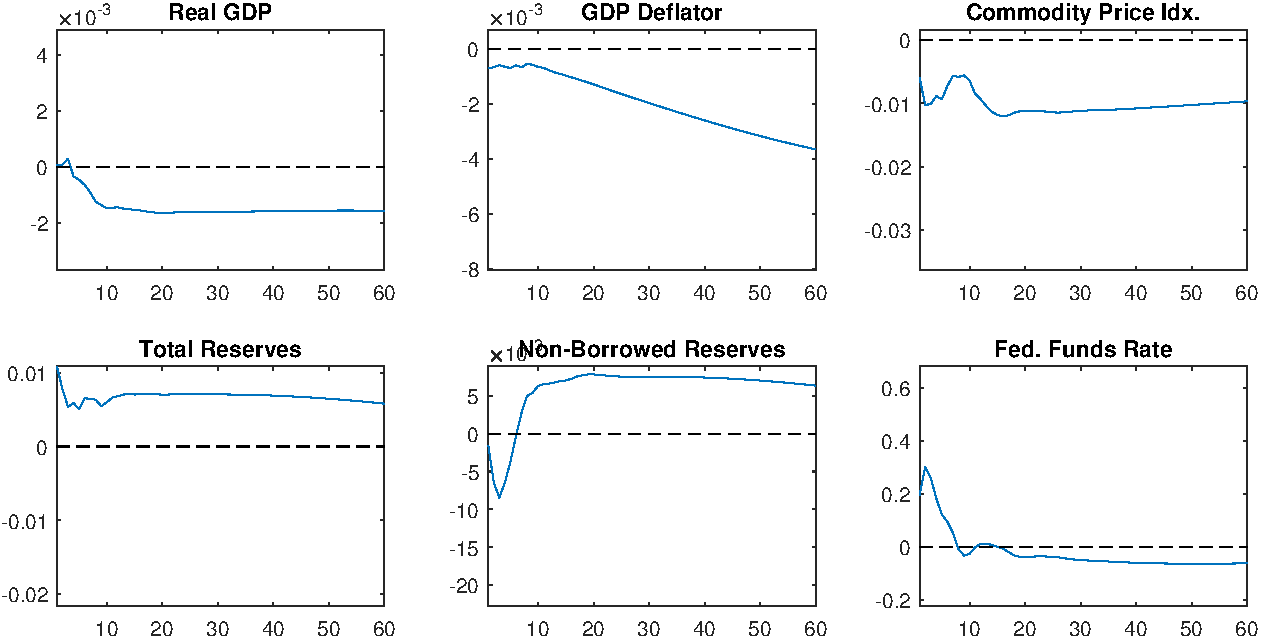
\includegraphics[width=.8\textwidth]{Uhlig_Replication_1rot.pdf}
\end{figure}
\end{frame}

%------------------------------------------

\begin{frame}
{\textbf{What happens when you do sign restrictions }}

\begin{itemize}
\item Start drawing $Q$ again until you find another one...
\end{itemize}

\begin{figure}[h]
\vspace{.3cm}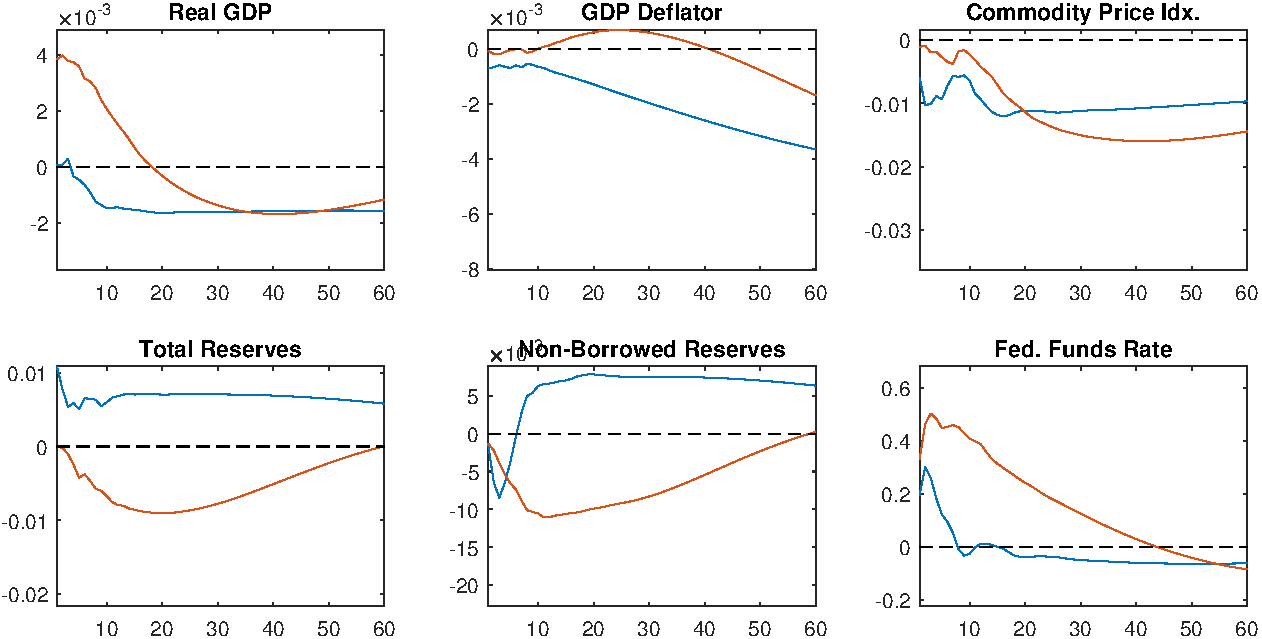
\includegraphics[width=.8\textwidth]{Uhlig_Replication_2rot.pdf}
\end{figure}
\end{frame}

%------------------------------------------

\begin{frame}
{\textbf{What happens when you do sign restrictions }}

\begin{itemize}
\item After a while...
\end{itemize}

\begin{figure}[h]
\vspace{.3cm}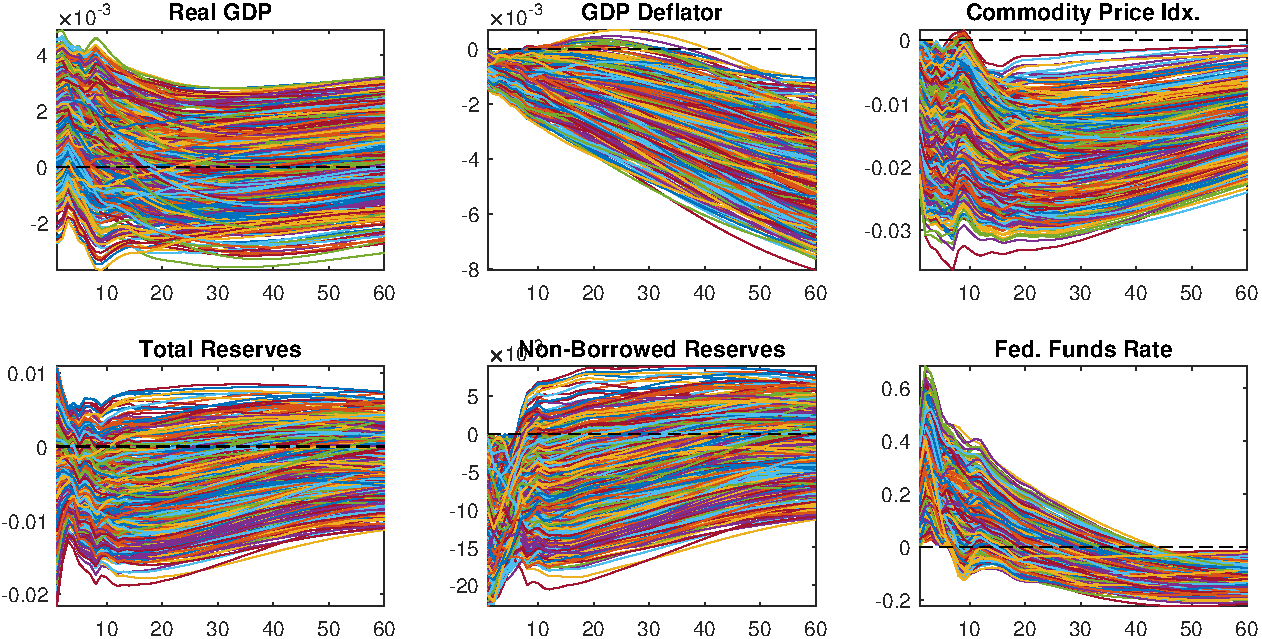
\includegraphics[width=.8%
\textwidth]{Uhlig_Replication_500rot.pdf}
\end{figure}
\end{frame}

%------------------------------------------

\begin{frame}
{\textbf{What are the effects of monetary policy on output?}}

\begin{itemize}
\item Ambiguous effect on real GDP $\Longrightarrow $\ Long-run monetary
neutrality
\end{itemize}

\begin{figure}[h]
\vspace{.3cm}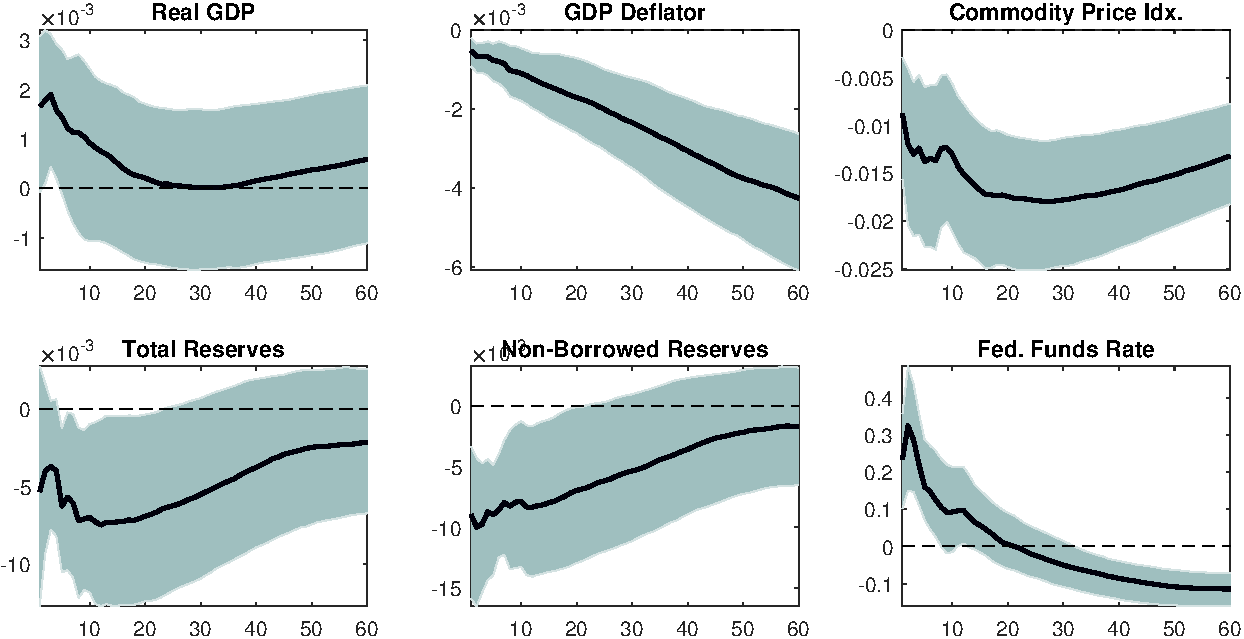
\includegraphics[width=.8\textwidth]{Uhlig_Replication.pdf}
\end{figure}
\end{frame}

%------------------------------------------

\subsection{Gertler and Karadi (2015)}

\begin{frame}
\vspace{3cm} \color{title}\centering{\huge \textbf{Practical Examples}}%
\bigskip

\color{note}\centering{\Large \textbf{Gertler and Karadi (2015, AEJ:M)}}
\end{frame}

%------------------------------------------

\subsection{Cesa-Bianchi and Sokol (2020)}

\begin{frame}
\vspace{3cm} \color{title}\centering{\huge \textbf{Practical Examples}}%
\bigskip

\color{note}\centering{\Large \textbf{Cesa-Bianchi and Sokol (2020)}}
\end{frame}

%------------------------------------------

\end{document}
